\documentclass[11pt,a4paper,openany]{report}
\usepackage[utf8]{inputenc}
\usepackage[T1]{fontenc}
\usepackage[ngerman]{babel}
\usepackage{lmodern}
\usepackage{microtype}
\usepackage{amsmath,amssymb,mathtools}
\usepackage[a4paper,margin=2.4cm,headheight=14pt]{geometry}
\usepackage{booktabs,tabularx,array,longtable,multirow}
\usepackage[shortlabels]{enumitem}
\usepackage{xcolor}
\usepackage{tikz}
\usetikzlibrary{arrows.meta,calc,patterns,decorations.pathreplacing,positioning,shapes.geometric}
\usepackage{listings}
\usepackage[htt]{hyphenat}
\usepackage[most]{tcolorbox}
\usepackage{fancyhdr}
\usepackage{makeidx}
\makeindex
\usepackage{titlesec}
\usepackage[colorlinks=true,linkcolor=blue!50!black,urlcolor=blue!50!black,citecolor=blue!50!black,
            pdftitle={FourierGrating -- Benutzerhandbuch},pdfauthor={FourierGrating-Projekt}]{hyperref}

% ------------------------------------------------------------------ Farben, Boxen
\definecolor{fgblue}{RGB}{31,73,125}
\definecolor{fggray}{RGB}{245,246,248}
\definecolor{fgkey}{RGB}{140,30,30}
\definecolor{fgstr}{RGB}{20,110,40}
\newtcolorbox{hinweis}[1][Hinweis]{colback=blue!3,colframe=fgblue,fonttitle=\bfseries\small,
  fontupper=\small,title={#1},left=5pt,right=5pt,top=3pt,bottom=3pt,breakable}
\newtcolorbox{achtung}[1][Achtung]{colback=red!3,colframe=red!55!black,fonttitle=\bfseries\small,
  fontupper=\small,title={#1},left=5pt,right=5pt,top=3pt,bottom=3pt,breakable}
\newtcolorbox{tipp}[1][Tipp]{colback=green!3,colframe=green!40!black,fonttitle=\bfseries\small,
  fontupper=\small,title={#1},left=5pt,right=5pt,top=3pt,bottom=3pt,breakable}

% ------------------------------------------------------------------ Listings
\lstdefinelanguage{json}{
  morestring=[b]",
  stringstyle=\color{fgstr},
  comment=[l]{//},
  commentstyle=\color{gray}\itshape,
  literate=
   {ä}{{\"a}}1 {ö}{{\"o}}1 {ü}{{\"u}}1 {Ä}{{\"A}}1 {Ö}{{\"O}}1 {Ü}{{\"U}}1 {ß}{{\ss}}1
   {µ}{{$\mu$}}1 {λ}{{$\lambda$}}1 {φ}{{$\varphi$}}1 {ψ}{{$\psi$}}1 {δ}{{$\delta$}}1 {×}{{$\times$}}1
   {→}{{$\to$}}1 {≥}{{$\geq$}}1 {≤}{{$\leq$}}1 {–}{{--}}1 {ε}{{$\varepsilon$}}1 {η}{{$\eta$}}1
}
\lstset{
  basicstyle=\ttfamily\small,
  backgroundcolor=\color{fggray},
  frame=single,framerule=0pt,
  xleftmargin=4pt,xrightmargin=4pt,
  aboveskip=6pt,belowskip=6pt,
  columns=fullflexible,keepspaces=true,
  breaklines=true,breakatwhitespace=false,
  showstringspaces=false,
  upquote=true,
  keywordstyle=\color{fgblue}\bfseries,
  commentstyle=\color{gray}\itshape,
  stringstyle=\color{fgstr},
  literate=
   {ä}{{\"a}}1 {ö}{{\"o}}1 {ü}{{\"u}}1 {Ä}{{\"A}}1 {Ö}{{\"O}}1 {Ü}{{\"U}}1 {ß}{{\ss}}1
   {µ}{{$\mu$}}1 {λ}{{$\lambda$}}1 {φ}{{$\varphi$}}1 {ψ}{{$\psi$}}1 {δ}{{$\delta$}}1 {×}{{$\times$}}1
   {→}{{$\to$}}1 {≥}{{$\geq$}}1 {≤}{{$\leq$}}1 {–}{{--}}1 {ε}{{$\varepsilon$}}1 {η}{{$\eta$}}1
   {Σ}{{$\Sigma$}}1 {−}{{-}}1
}
\lstdefinestyle{shell}{language=bash,morekeywords={cmake,ctest,pip,fgsolve,python,sudo,git,pytest}}
\lstdefinestyle{py}{language=Python}
\lstdefinestyle{cpp}{language=C++}

% ------------------------------------------------------------------ Kurzbefehle
% Schlüssel erscheinen im Stichwortverzeichnis (außer Kurzformen wie .z, die mit einem Punkt beginnen)
\makeatletter
\def\fg@keyindex#1#2\relax{\ifx.#1\else\index{#1#2@\texttt{#1#2}}\fi}
\newcommand{\key}[1]{\texttt{\textcolor{fgkey}{#1}}\fg@keyindex#1\relax}
\makeatother
\newcolumntype{Y}{>{\raggedright\arraybackslash}X}
\let\fgus\_
\renewcommand{\_}{\fgus\allowbreak}

\newcommand{\val}[1]{\texttt{#1}}
\newcommand{\file}[1]{\texttt{#1}}
\newcommand{\cmd}[1]{\texttt{#1}}
\newcommand{\um}{\,\textmu m}
\newcommand{\FG}{\textsf{FourierGrating}}
\newcommand{\GUI}{\textsf{GUI-FourierGrating}}
\newcommand{\gui}[1]{\textsf{\bfseries #1}}
\setlength{\parindent}{0pt}
\setlength{\parskip}{4pt plus 1pt}
\renewcommand{\arraystretch}{1.15}

% ------------------------------------------------------------------ Kopfzeilen
\pagestyle{fancy}
\fancyhf{}
\fancyhead[L]{\small\textsf{FourierGrating -- Benutzerhandbuch}}
\fancyhead[R]{\small\nouppercase{\leftmark}}
\fancyfoot[C]{\small\thepage}
\renewcommand{\headrulewidth}{0.4pt}
\fancypagestyle{plain}{\fancyhf{}\fancyfoot[C]{\small\thepage}\renewcommand{\headrulewidth}{0pt}}
\titleformat{\chapter}[display]{\normalfont\sffamily\bfseries\color{fgblue}}
  {\large \chaptertitlename\ \thechapter}{4pt}{\huge}
\titlespacing*{\chapter}{0pt}{0pt}{18pt}
\titleformat*{\section}{\normalfont\sffamily\Large\bfseries\color{fgblue}}
\titleformat*{\subsection}{\normalfont\sffamily\large\bfseries}
\titleformat*{\subsubsection}{\normalfont\sffamily\normalsize\bfseries}
\setcounter{tocdepth}{1}

\begin{document}
% " ist in JSON-Werten ein Anführungszeichen, kein babel-Kürzel (sonst wird "auto" zu äuto")
\shorthandoff{"}

% ------------------------------------------------------------------ Titelseite
\begin{titlepage}
\centering
\vspace*{3cm}
{\sffamily\bfseries\color{fgblue}\fontsize{38}{44}\selectfont FourierGrating\par}
\vspace{0.6cm}
{\sffamily\Large Benutzerhandbuch\par}
\vspace{1.4cm}
\begin{tikzpicture}[scale=1.0]
  \fill[blue!10] (-4,-1.2) rectangle (4,0);
  \foreach \x in {-4,-3,...,3} \fill[fgblue!60] (\x,0) rectangle (\x+0.45,0.6);
  \draw[thick] (-4,0) -- (4,0);
  \draw[-{Latex[length=3mm]},very thick,red!70!black] (-2.2,2.6) -- (-0.3,0.7);
  \foreach \a/\l in {60/R_{-1},90/R_0,120/R_{+1}}
    \draw[-{Latex[length=2.5mm]},thick,fgblue] (0.2,0.7) -- ++(\a:1.9);
  \foreach \a/\l in {-70/,-95/,-120/}
    \draw[-{Latex[length=2.5mm]},thick,fgblue!60] (0.2,-1.2) -- ++(\a:1.0);
\end{tikzpicture}
\vspace{1.4cm}

{\large Beugung elektromagnetischer Wellen an periodischen und isolierten Strukturen\\
mit der Fourier-Modal-Methode\\[4pt]
Differentialmethode (implizites Runge--Kutta) und RCWA\par}
\vfill
{\small
\begin{tabular}{rl}
Programmstand: & FourierGrating 0.20 (Repository-Stand 18.\,11.\,2026)\\
               & GUI-FourierGrating 0.10\\
Spezifikation: & Implementierungsplan Version 2.24 (\file{docs/implementation\_plan/main.pdf})\\
Lizenz:        & MIT
\end{tabular}\par}
\end{titlepage}

\pagenumbering{roman}
\tableofcontents
\clearpage
\pagenumbering{arabic}

\chapter{Einleitung}\label{ch:einleitung}

\section{Was ist FourierGrating?}
\FG{} berechnet, wie eine elektromagnetische Welle an einer \emph{periodisch strukturierten} Oberfläche oder
einem Schichtstapel gebeugt wird. Typische Ergebnisse sind
\begin{itemize}
  \item die \textbf{Beugungseffizienzen} aller reflektierten und transmittierten Ordnungen, getrennt nach s- und
        p-Anteil, mit komplexen Amplituden,
  \item die \textbf{Absorption} und die Energiebilanz,
  \item \textbf{Nahfelder} ($\mathbf E$, $\mathbf H$, $|\mathbf E|^2$, Poynting-Vektor) in Schnitten durch die Struktur,
  \item bei isolierten Strukturen \textbf{Streubreiten und Streuquerschnitte}, bei Wellenleitern die Leistung
        geführter \textbf{Moden},
  \item \textbf{Gradienten} beliebiger Zielfunktionen der Effizienzen nach Geometrie-, Material- und
        Einfallsparametern, für die Optimierung.
\end{itemize}

Das Programm löst die Maxwellgleichungen mit der \textbf{Fourier-Modal-Methode (FMM)}. Die Felder werden in den
periodischen Richtungen in Fourierreihen entwickelt; in der Schichtrichtung $y$ entsteht ein System gewöhnlicher
Differentialgleichungen $\mathrm dF/\mathrm dy = M(y)\,F$. \FG{} bietet zwei Wege, es zu lösen:

\begin{description}
  \item[RCWA] (\emph{Rigorous Coupled-Wave Analysis}): Die Struktur wird in Scheiben zerlegt, in denen $M$ nicht von
        $y$ abhängt. In jeder Scheibe wird ein Eigenwertproblem gelöst. Das ist ideal für Strukturen mit senkrechten
        Wänden (Lamellen, Säulen, Löcher).
  \item[Differentialmethode] mit \textbf{implizitem Runge--Kutta-Verfahren} (Gauß--Legendre, Radau~IIA): $M(y)$ wird
        direkt integriert. Das ist ideal für Profile mit schrägen oder gekrümmten Flanken (Sinus- und
        Echelettegitter), weil keine Treppenstufen entstehen.
\end{description}
Beide Wege verwenden die \textbf{schnelle Fourierfaktorisierung} (\emph{Fast Fourier Factorization}, FFF) nach
Nevière und Popov mit Normalenvektorfeldern. Sie sorgt dafür, dass auch Metallgitter in TM-Polarisation schnell
konvergieren.

\section{Funktionsumfang im Überblick}
\begin{center}
\small
\begin{tabularx}{\linewidth}{>{\raggedright\arraybackslash}p{4.1cm}X}
\toprule
Bereich & Möglichkeiten \\
\midrule
Geometrie & 1D-Gitter (periodisch in $x$), 2D-Gitter (periodisch in $x$ und $z$), isolierte Strukturen mit PML,
rotationssymmetrische Strukturen (in Arbeit) \\
Schichttypen & homogen, Lamellen, Profile $y=g(x)$ (Sinus, Dreieck, Spline), Polygone, gekrümmte Konturen (Kreis,
Ellipse, NURBS), Profile $y=g(x,z)$, STEP-Körper aus CAD, Ringe \\
Materialien & isotrop (reell oder komplex), anisotrop mit vollem $\varepsilon$-Tensor oder Hauptwerten und
Euler-Winkeln; Metalle, Dielektrika, Halbleiter \\
Einfall & ebene Welle beliebiger Richtung und Polarisation (auch konisch), Gauß-Strahl (Zylinderpfad), geführte Mode
eines strukturierten Halbraums \\
Löser & RCWA und Runge--Kutta; Faktorisierungen Laurent, Li, FFF in mehreren Varianten; adaptive räumliche Auflösung
(ASR) \\
Auswertung & Effizienzen, s/p-Anteile, Amplituden, S-Matrix in der s/p-Basis, Nahfelder, Streuquerschnitte,
Modenleistungen \\
Scans & Wellenlänge, Winkel und Polarisation als Liste oder Bereich (kartesisches Produkt); Sweep über beliebige Zahlen
der Konfiguration \\
Optimierung & exakte Gradienten über die diskrete Adjungierte; Adapter für PyTorch und JAX \\
Leistung & OpenMP-Parallelisierung auf drei Ebenen, CUDA-Backend für NVIDIA-GPUs, wählbare Genauigkeit
(fp64/mixed/fp32) \\
Schnittstellen & Kommandozeile \cmd{fgsolve}, Python-Paket \texttt{fouriergrating}, C++-Bibliothek, grafische
Oberfläche im Browser (\GUI) \\
\bottomrule
\end{tabularx}
\end{center}

\section{Was FourierGrating (noch) nicht kann}
\begin{itemize}
  \item \textbf{Dispersive Materialien}: Ein Material hat für alle Wellenlängen eines Scans dieselbe Brechzahl.
        Für Spektren über einen größeren Bereich ist das bei Metallen und Halbleitern falsch. Abhilfe bis zur
        Umsetzung (Meilenstein M22, geplant): je Wellenlänge eine Rechnung mit passender Brechzahl, am bequemsten in
        Python (Abschnitt~\ref{sec:py-dispersion}).
  \item Nichtlineare Optik, magnetische Materialien ($\mu_r\neq1$), zeitabhängige Felder.
  \item Kurvenförmige Schichtgrenzen in $y$-Richtung außerhalb der unterstützten Profil- und CAD-Typen.
  \item Rotationssymmetrische Strukturen (Meilenstein M20) sind teilweise umgesetzt; Nahfeld, Profile in Ringform
        und CAD-Rotationskörper folgen. $P$-zählige Drehsymmetrie (M21) ist spezifiziert, aber noch nicht umgesetzt.
\end{itemize}

\section{Aufbau dieses Handbuchs}
\begin{center}
\small
\begin{tabularx}{\linewidth}{lY}
\toprule
Kapitel & Inhalt \\
\midrule
\ref{ch:grundlagen} & Physikalische Grundlagen, Koordinaten, Definitionen -- \emph{einmal lesen} \\
\ref{ch:installation}, \ref{ch:schnellstart} & Installation und erste Rechnung \\
\ref{ch:konfiguration}--\ref{ch:ausgabe} & Konfigurationsdatei, Schichttypen, Löserwahl, Scans, Nahfeld, Ausgaben
-- \emph{das Nachschlagewerk} \\
\ref{ch:erweitert}, \ref{ch:cad} & Isolierte Strukturen, ASR, Zylinderkoordinaten, CAD-Import \\
\ref{ch:python}, \ref{ch:optimierung}, \ref{ch:cpp} & Programmierschnittstellen und Optimierung \\
\ref{ch:leistung} & Rechenzeit, Parallelisierung, GPU, Genauigkeit \\
\ref{ch:gui} & Grafische Oberfläche im Browser \\
\ref{ch:rezepte} & Durchgerechnete Beispiele \\
\ref{ch:probleme} & Fehlermeldungen und Fehlersuche \\
Anhang & Schlüsselreferenz, Umgebungsvariablen, Referenzfälle, Glossar, Literatur \\
\bottomrule
\end{tabularx}
\end{center}

\section{Darstellung}
\begin{itemize}
  \item Schlüssel der Konfigurationsdatei erscheinen als \key{lambda\_um}, Werte als \val{"rcwa"}, Dateien als
        \file{examples/v3\_lamellar\_dielectric.json}, Befehle als \cmd{fgsolve}.
  \item Pfade sind relativ zum Wurzelverzeichnis des Repositorys \file{FourierGrating}, sofern nicht anders gesagt.
  \item Einheiten: Längen immer in Mikrometern (\textmu m), Winkel in Grad. Das gilt für die Konfiguration, die
        Python-Schnittstelle und die GUI gleichermaßen.
  \item Kommentare mit \texttt{//} in JSON-Beispielen dienen nur der Erklärung. Echte Konfigurationsdateien sind
        reines JSON ohne Kommentare.
\end{itemize}

\begin{hinweis}[Verbindliche Quelle]
Alle Formeln, Algorithmen und Abnahmekriterien stehen im \textbf{Implementierungsplan}
(\file{docs/implementation\_plan/main.pdf}). Dieses Handbuch erklärt die \emph{Benutzung}. Wo es Formeln nennt,
verweist es auf den Plan; bei einem Widerspruch gilt der Plan bzw.\ das tatsächliche Verhalten des Programms.
\end{hinweis}

\chapter{Physikalische Grundlagen und Konventionen}\label{ch:grundlagen}

Dieses Kapitel legt fest, wie \FG{} Geometrie, Einfall und Ergebnisse beschreibt. Wer die Konventionen kennt,
liest jede Konfigurationsdatei und jede Ergebnistabelle ohne Rätselraten.

\section{Koordinatensystem und Schichtstapel}
\index{Koordinatensystem}\index{Schichtstapel}%
\begin{figure}[h]
\centering
\begin{tikzpicture}[scale=1.05,>=Latex]
  % Substrat
  \fill[gray!25] (0,-1.6) rectangle (9,0);
  \node at (7.6,-0.8) {\small Substrat (Medium 1), $y<0$};
  % Schicht 1: homogen
  \fill[blue!12] (0,0) rectangle (9,0.5);
  \node[anchor=west] at (9.1,0.25) {\small Schicht 1};
  % Schicht 2: Lamellen
  \foreach \x in {0,3,6} \fill[blue!45] (\x,0.5) rectangle (\x+1.4,1.3);
  \node[anchor=west] at (9.1,0.9) {\small Schicht 2};
  % Schicht 3: Profil
  \fill[blue!25] (0,1.3) -- plot[domain=0:9,samples=60] (\x,{1.3+0.25*(1+cos(120*\x))}) -- (9,1.3) -- cycle;
  \node[anchor=west] at (9.1,1.6) {\small Schicht 3};
  \node at (7.6,2.9) {\small Superstrat (Medium $M$)};
  \draw[thick] (0,0) -- (9,0);
  % Periode
  \draw[decorate,decoration={brace,amplitude=4pt,mirror}] (0,-1.75) -- (3,-1.75)
     node[midway,below=4pt] {\small Periode $d_x$};
  % Achsen
  \draw[->,thick] (-1.9,-1.5) -- (-0.9,-1.5) node[right] {$x$};
  \draw[->,thick] (-1.9,-1.5) -- (-1.9,-0.5) node[above] {$y$};
  \draw[->,thick] (-1.9,-1.5) -- (-2.45,-1.9) node[below left] {$z$};
  \fill (-1.9,-1.5) circle (1.2pt);
  % Einfall
  \draw[->,very thick,red!70!black] (3.0,3.9) -- (4.2,2.4) node[midway,left] {\small $\mathbf k_{\text{inc}}$};
  \draw[dashed] (4.2,2.4) -- (4.2,3.9);
  \draw (4.2,3.3) arc (90:128:0.9);
  \node at (3.85,3.45) {\small$\varphi$};
  % y=0
  \node[anchor=east] at (-0.05,0) {\small $y=0$};
\end{tikzpicture}
\caption{Koordinaten und Schichtstapel. Licht fällt von oben aus dem Superstrat ein. Schichten werden von unten
(Substratseite) nach oben gezählt.}
\label{fig:koordinaten}
\end{figure}

\begin{itemize}
  \item Die \textbf{Schichtnormale ist $y$}. Die Grenze zum Substrat liegt bei $y=0$, $y$ wächst nach oben.
  \item Die Struktur ist periodisch in $x$ mit der Periode $d_x$ (\key{period\_um.x}) und bei 2D-Gittern zusätzlich
        in $z$ mit $d_z$ (\key{period\_um.z}). Bei 1D-Gittern hängt nichts von $z$ ab.
  \item Unten liegt das \textbf{Substrat} (Medium 1, \key{substrate}), oben das \textbf{Superstrat} (Medium $M$,
        \key{superstrate}). Beide sind Halbräume.
  \item Die \textbf{Schichten} (\key{layers}) werden \emph{von unten nach oben} aufgezählt. Die erste Schicht liegt
        direkt auf dem Substrat.
  \item Das Licht fällt \textbf{von oben} aus dem Superstrat ein. Das Superstrat muss deshalb verlustfrei sein
        (reelle Brechzahl $\nu_M$).
\end{itemize}

\section{Zeitkonvention und Materialangaben}
\index{Zeitkonvention}\index{Vorzeichenkonvention|see{Zeitkonvention}}%
\FG{} verwendet die Zeitabhängigkeit $e^{-i\omega t}$. Daraus folgt:
\begin{itemize}
  \item Eine komplexe Brechzahl $\nu = n + ik$ beschreibt Absorption, wenn $k>0$ ist. Gold bei 633\,nm ist etwa
        $\nu = 0{,}2+3{,}4i$, in der Konfiguration \val{[0.2, 3.4]}.
  \item Die relative Permittivität ist $\varepsilon=\nu^2$; verlustbehaftete Medien haben
        $\operatorname{Im}\varepsilon>0$.
  \item Magnetische Materialien gibt es nicht: $\mu_r = 1$ überall.
\end{itemize}
Intern rechnet \FG{} in normierten Einheiten ($k_0 = 2\pi/\lambda = 1$, $\tilde{\mathbf H} = Z_0\mathbf H$). Davon
merkt man als Anwender nur, dass ausgegebene Magnetfelder mit $Z_0$ multipliziert sind (Abschnitt~\ref{sec:nf-dateien}).

\section{Einfallsrichtung und Polarisation}\label{sec:einfall}
\index{Polarisation}\index{Einfallswinkel}\index{konischer Einfall}%
Eine ebene Welle im Superstrat mit Brechzahl $\nu=\nu_M$ wird durch vier Größen beschrieben:
\begin{center}
\begin{tabular}{lll}
\toprule
Größe & Schlüssel & Bedeutung \\
\midrule
$\lambda$ & \key{lambda\_um} & Vakuumwellenlänge in \textmu m \\
$\varphi$ & \key{phi\_deg} & Polarwinkel gegen die Normale $y$ ($0^\circ$ = senkrechter Einfall) \\
$\psi$ & \key{psi\_deg} & Azimut der Einfallsebene gegen die $x$-Achse ($0^\circ$: Einfallsebene $= xy$-Ebene) \\
$\delta$ & \key{delta\_deg} & Polarisationswinkel: $0^\circ$ = s (TE), $90^\circ$ = p (TM) \\
\bottomrule
\end{tabular}
\end{center}
Der Wellenvektor ist (normiert auf $k_0$)
\begin{equation}
  \mathbf k_{\text{inc}} = (\alpha_0,\,-\beta_0,\,\gamma_0),\qquad
  \alpha_0 = \nu\sin\varphi\cos\psi,\quad \beta_0 = \nu\cos\varphi,\quad \gamma_0=\nu\sin\varphi\sin\psi .
\end{equation}
\begin{itemize}
  \item \textbf{Klassischer Einfall}: $\psi=0$. Bei 1D-Gittern liegen dann alle Beugungsordnungen in der Einfallsebene,
        und TE und TM entkoppeln (bei isotropen Materialien).
  \item \textbf{Konischer Einfall}: $\psi\neq0$. Die Ordnungen verlassen die Einfallsebene, s und p koppeln.
  \item \textbf{Polarisation}: $\delta=0^\circ$ heißt, $\mathbf E$ steht senkrecht auf der Einfallsebene
        (s, bei $\psi=0$: TE, $\mathbf E\parallel z$). $\delta=90^\circ$ heißt p (TM). Zwischenwerte ergeben linear
        polarisiertes Licht mit Anteilen beider.
  \item Bei senkrechtem Einfall ($\varphi=0$) ist die Einfallsebene nicht eindeutig; sie wird dann durch $\psi$
        festgelegt.
\end{itemize}

\section{Beugungsordnungen und Gittergleichung}
\index{Beugungsordnung}\index{Gittergleichung}\index{Rayleigh-Anomalie}%
Wegen der Periodizität enthält das Feld nur die Tangentialkomponenten
\begin{equation}
  \alpha_n = \alpha_0 + n\,\frac{\lambda}{d_x},\qquad \gamma_m = \gamma_0 + m\,\frac{\lambda}{d_z}
  \qquad (n,m\in\mathbb Z),
\end{equation}
also die \textbf{Beugungsordnungen} $(n,m)$. In 1D ist stets $m=0$. In einem homogenen Medium mit Brechzahl $\nu_j$
gehört dazu die Normalkomponente
\begin{equation}
  \beta_{nm}^{(j)}=\sqrt{\nu_j^2-\alpha_n^2-\gamma_m^2},\qquad \operatorname{Im}\beta\ge0 .
\end{equation}
Ist $\beta$ reell, \textbf{propagiert} die Ordnung und trägt Leistung ab; sonst ist sie evaneszent. In der Ausgabe
erscheinen nur propagierende Ordnungen. Für den klassischen Einfall auf ein 1D-Gitter ist das die bekannte
Gittergleichung $\nu_j\sin\theta_n = \nu_M\sin\varphi + n\lambda/d_x$.

\begin{tipp}[Littrow-Anordnung]
Fällt die Ordnung $-1$ genau in sich zurück, gilt $2\,d_x\,\nu_M\sin\varphi = \lambda$. Beispiel: $d_x=0{,}5$\um,
$\lambda=0{,}6328$\um{} ergibt $\varphi\approx 39{,}3^\circ$.
\end{tipp}

\section{Effizienzen und Energiebilanz}
\index{Effizienz}\index{Energiebilanz}%
Die \textbf{Beugungseffizienz} einer Ordnung ist der Anteil des einfallenden Leistungsflusses (Poynting-Vektor in
$y$-Richtung), den diese Ordnung abführt:
\begin{equation}
  e^{R}_{nm} = \frac{P^{\uparrow}_{nm}}{P_{\text{inc}}},\qquad e^{T}_{nm} = \frac{P^{\downarrow}_{nm}}{P_{\text{inc}}} .
\end{equation}
Die Summe über alle propagierenden Ordnungen ergibt mit der \textbf{Absorption} $A$:
\begin{equation}
  \sum e^R + \sum e^T + A = 1 .
\end{equation}
\begin{itemize}
  \item Sind alle Materialien verlustfrei, muss $A=0$ sein. Die Größe \texttt{sum R+T} in der Ausgabe ist dann ein
        guter Gütetest der Rechnung (Abschnitt~\ref{sec:diagnose}).
  \item Ist das Substrat absorbierend, gibt es keine transmittierten Ordnungen; dann ist $A = 1-\sum e^R$.
  \item In isotropen Halbräumen zerlegt \FG{} jede Ordnung zusätzlich in s- und p-Anteil (\texttt{eff\_s},
        \texttt{eff\_p}) und gibt die komplexen Amplituden aus (\texttt{amp\_s}, \texttt{amp\_p}).
\end{itemize}

\section{Wie die Fourier-Modal-Methode rechnet}
\index{Fourier-Modal-Methode}%
\subsection{Fourierreihen und Trunkierung}
In jeder Schicht werden $\varepsilon(x,z)$ und die Felder in Fourierreihen entwickelt und bei den Ordnungen
$-N_x\ldots N_x$ (und $-N_z\ldots N_z$) abgeschnitten. Die Zahl der Fourierordnungen ist
\begin{equation}
  n_f = (2N_x+1)(2N_z+1),
\end{equation}
und die Systemmatrizen haben die Größe $n=4n_f$ (je zwei tangentiale Komponenten von $\mathbf E$ und $\mathbf H$).
Die Rechenzeit wächst ungefähr mit $n^3$, der Speicher mit $n^2$. $N_x$ und $N_z$ werden mit \key{truncation}
festgelegt und sind der wichtigste Genauigkeitsparameter (Kapitel~\ref{ch:loeser}).

\subsection{RCWA}
In einer Schicht, deren Querschnitt nicht von $y$ abhängt, ist $M$ konstant. Die Lösung ist eine Summe von
Eigenmoden. \FG{} löst das Eigenwertproblem je Schicht und verkettet die Schichten über S-Matrizen
(Sternprodukt), was auch bei dicken Metallschichten stabil ist. Profile werden für die RCWA in
\key{slices} waagerechte Scheiben zerlegt (Treppennäherung).

\subsection{Differentialmethode (Runge--Kutta)}
Bei Profilen hängt $M$ stetig von $y$ ab. Das Runge--Kutta-Verfahren integriert $\mathrm dF/\mathrm dy=M(y)F$ mit
Schrittweitensteuerung (Toleranz \key{rk.tol}) und ohne Treppe. Instabilitäten durch exponentiell wachsende Moden
fängt eine automatische Zerlegung in Stabilitätsscheiben ab, die wieder über S-Matrizen verkettet werden.

\subsection{Faktorisierung}
Das Produkt $\varepsilon\cdot E$ an einer Materialgrenze ist das Kernproblem jeder FMM: $E_\perp$ springt dort,
$D_\perp=\varepsilon E_\perp$ ist stetig. Die naive Fourierfaktorisierung (Laurent) konvergiert deshalb in TM sehr
langsam. Die korrekten Regeln (Li) bzw.\ ihre Verallgemeinerung auf beliebige Formen mit einem Normalenvektorfeld
(FFF) beheben das. \FG{} wählt mit \val{"auto"} je Schichttyp die passende Variante (Tabelle~\ref{tab:faktorisierung}).

\section{Was „konvergiert“ heißt}
\index{Konvergenz}%
Jede FMM-Rechnung ist eine Näherung, die mit wachsendem $N$ (und bei RCWA-Profilen mit wachsender Scheibenzahl,
bei RK mit kleinerer Toleranz) gegen das exakte Ergebnis strebt. Ein einzelnes Ergebnis sagt daher nichts über seine
Genauigkeit aus. \textbf{Prüfen Sie Konvergenz immer}, indem Sie dieselbe Rechnung mit zwei bis drei Werten von $N$
wiederholen (Abschnitt~\ref{sec:konvergenz}).

\chapter{Installation}\label{ch:installation}

\FG{} gibt es in drei Formen. Welche Sie brauchen, hängt davon ab, wie Sie arbeiten möchten:
\begin{center}
\small
\begin{tabularx}{\linewidth}{lYl}
\toprule
Form & geeignet für & Abschnitt \\
\midrule
Python-Paket \texttt{fouriergrating} & Skripte, Jupyter, Optimierung, die meisten Anwender & \ref{sec:inst-python} \\
Kommandozeile \cmd{fgsolve} (C++-Build) & Rechnungen aus JSON-Dateien, Server, Batchbetrieb & \ref{sec:inst-linux}, \ref{sec:inst-windows} \\
GUI im Browser & Arbeiten ohne Programmierung, gemeinsamer Rechenserver & \ref{sec:inst-gui}, Kapitel~\ref{ch:gui} \\
\bottomrule
\end{tabularx}
\end{center}

\section{Systemvoraussetzungen}
\begin{itemize}
  \item \textbf{Zielsystem}: AlmaLinux 10 (x86\_64) mit GCC 14, optional NVIDIA RTX 6000 Ada (sm\_89, 48\,GB).
  \item \textbf{Anwenderinstallation}: Windows 11, optional mit NVIDIA RTX 3090 (sm\_86, 24\,GB).
  \item Mindestversionen für den Quellbuild: CMake 3.24, GCC 13 (C++20), für CUDA das Toolkit 12.6 Update~2
        (wegen \texttt{cusolverDnXgeev}).
  \item Abhängigkeiten: Eigen 3.4, nlohmann/json, GoogleTest (nur Tests), optional OpenMP, CUDA, HDF5, Nurbforge
        (CAD). Fehlende Bibliotheken lädt CMake beim ersten Konfigurieren über \texttt{FetchContent} nach; dafür ist
        Internetzugang nötig.
  \item Arbeitsspeicher: Eine 2D-Rechnung mit $N_x=N_z=10$ hat Matrizen der Größe $n = 4\cdot441=1764$; je komplexer
        Matrix sind das rund 50\,MB, gleichzeitig werden etwa zwölf davon je Scanpunkt gebraucht.
\end{itemize}

\section{Python-Paket}\label{sec:inst-python}
\index{Installation!Python-Paket}%
\begin{center}
\small
\begin{tabularx}{\linewidth}{lY}
\toprule
Umgebung & Befehl \\
\midrule
Windows 11, CPU & \cmd{pip install fouriergrating} \\
Windows 11 mit RTX 3090 & zusätzlich \cmd{pip install fouriergrating-cuda12} (zieht die \texttt{nvidia-*-cu12}-Pakete) \\
Linux (manylinux\_2\_28), CPU & \cmd{pip install fouriergrating} \\
Server mit CUDA & aus den Quellen, siehe unten \\
Entwicklung & \cmd{pip install .} im Repository \\
\bottomrule
\end{tabularx}
\end{center}

Aus den Quellen mit CUDA (Server, RTX 6000 Ada):
\begin{lstlisting}[style=shell]
pip install . -C cmake.define.FG_ENABLE_CUDA=ON \
              -C cmake.define.CMAKE_CUDA_ARCHITECTURES="89"
\end{lstlisting}
Unter Windows braucht der Quellbuild MSVC 2022, weil Python mit MSVC gebaut ist:
\begin{lstlisting}[style=shell]
scripts\msvc.cmd python -m pip install .
scripts\msvc.cmd python -m pip install python/cuda12     # CUDA-Variante
\end{lstlisting}

\textbf{Installation prüfen.}
\begin{lstlisting}[style=shell]
python -c "import fouriergrating as fg; print(fg.__version__, fg.core_variant(), fg.cuda_available())"
\end{lstlisting}
\texttt{core\_variant()} meldet \val{"cpu"} oder \val{"cuda12"}. Ist das CUDA-Paket installiert und eine GPU
nutzbar, lädt \texttt{import fouriergrating} automatisch den CUDA-Kern. Mit der Umgebungsvariablen
\texttt{FG\_CORE=cpu} erzwingen Sie den CPU-Kern. Unter Windows sucht das Paket die CUDA-Bibliotheken in den
\texttt{nvidia-*-cu12}-Paketen und, falls gesetzt, unter \texttt{CUDA\_PATH}; sie werden nicht mitgeliefert.

\paragraph{Optionale Pakete.} \texttt{pandas} für \texttt{ScanResult.to\_pandas()}, \texttt{torch} bzw.\
\texttt{jax} für die Gradienten-Adapter, \texttt{scipy} für die Optimierungsbeispiele, \texttt{matplotlib} und
\texttt{numpy} für die Plot-Skripte.

\section{Quellbuild unter Linux (AlmaLinux 10)}\label{sec:inst-linux}
\index{Installation!Linux}\index{AlmaLinux}%
\subsection{Pakete}
\begin{lstlisting}[style=shell]
sudo ./scripts/setup_almalinux10.sh              # Compiler, CMake, Eigen, JSON, GTest, Python, LaTeX
sudo ./scripts/setup_almalinux10.sh --with-cuda  # zusätzlich CUDA-Toolkit (NVIDIA-Repo rhel10)
\end{lstlisting}
Das Skript aktiviert EPEL und CRB. Den Grafiktreiber installiert es \emph{nicht}; folgen Sie dafür dem NVIDIA Driver
Installation Guide (Abschnitt RHEL/Alma 10) und prüfen Sie mit \cmd{nvidia-smi}.

\subsection{Konfigurieren, bauen, testen}
\begin{lstlisting}[style=shell]
cmake --preset cpu-release && cmake --build --preset cpu-release
ctest --preset cpu-release                      # ca. 15-20 min auf einem Kern
./build/cpu-release/apps/fgsolve --info

# mit GPU
cmake --preset cuda-release && cmake --build --preset cuda-release
./build/cuda-release/apps/fgsolve --info        # "cuda backend: NVIDIA RTX 6000 Ada ..."
\end{lstlisting}

\subsection{Presets und Optionen}
\begin{center}
\small
\begin{tabularx}{\linewidth}{lY}
\toprule
Preset & Zweck \\
\midrule
\texttt{cpu-release} & Standard: CPU, optimiert, mit OpenMP \\
\texttt{cpu-debug} & Fehlersuche \\
\texttt{cpu-tsan} & ThreadSanitizer (Entwicklung) \\
\texttt{cuda-release} & mit CUDA-Backend, Architektur 89 voreingestellt \\
\texttt{cpu-cad} & mit CAD-Slicer (Nurbforge) \\
\texttt{win-release}, \texttt{win-cuda}, \texttt{win-cad} & Windows mit MSYS2/MinGW-w64 \\
\texttt{win-msvc}, \texttt{win-msvc-cuda} & Windows mit MSVC 2022 \\
\bottomrule
\end{tabularx}
\end{center}
CMake-Optionen: \texttt{FG\_ENABLE\_CUDA}, \texttt{FG\_ENABLE\_OPENMP} (Standard an), \texttt{FG\_ENABLE\_HDF5},
\texttt{FG\_ENABLE\_NURBFORGE}, \texttt{FG\_BUILD\_TESTS}, \texttt{FG\_WARNINGS\_AS\_ERRORS}. Für eine andere
GPU setzen Sie \texttt{CMAKE\_CUDA\_ARCHITECTURES} (RTX 3090: \val{86}).

\section{Quellbuild unter Windows}\label{sec:inst-windows}
\index{Installation!Windows}%
Für Entwickler gibt es einen Weg über MSYS2/MinGW-w64 (UCRT64):
\begin{lstlisting}[style=shell]
.\scripts\setup_windows.ps1                 # installiert MSYS2 (falls nötig) und die Werkzeuge
cmake --preset win-release
cmake --build --preset win-release
ctest --preset win-release
$env:PATH = "C:\msys64\ucrt64\bin;" + $env:PATH
.\build\win-release\apps\fgsolve.exe examples\v3_lamellar_dielectric.json
\end{lstlisting}
Das CUDA-Preset \texttt{win-cuda} ist experimentell. Für Python-Wheels und CUDA unter Windows ist MSVC der
empfohlene Weg (\texttt{win-msvc}, \texttt{win-msvc-cuda}). Einzelheiten: \file{docs/build\_windows.md}.

\section{CAD-Slicer}\label{sec:inst-cad}
\index{Installation!CAD-Slicer}\index{Nurbforge}%
STEP-Dateien liest \FG{} mit der Bibliothek Nurbforge. Sie wird nur mit \texttt{FG\_ENABLE\_NURBFORGE=ON}
eingebunden (Tag \texttt{FG\_NURBFORGE\_TAG}, Standard \texttt{v0.6.0}):
\begin{lstlisting}[style=shell]
cmake --preset cpu-cad && cmake --build --preset cpu-cad
# lokale Nurbforge-Kopie statt Download:
cmake --preset cpu-cad -DFETCHCONTENT_SOURCE_DIR_NURBFORGE=/pfad/zu/Nurbforge
\end{lstlisting}
Die Python-Wheels enthalten den Slicer bereits. Ohne ihn meldet eine \val{"cad"}-Schicht \texttt{NotImplemented};
\cmd{fgsolve -{}-info} zeigt, ob er eingebaut ist.

\section{Grafische Oberfläche}\label{sec:inst-gui}
Die GUI ist ein eigenes Repository (\file{PhotonPower/GUI-FourierGrating}) und läuft als Webanwendung
(Streamlit) auf einem Server. Für Anwender genügt ein Browser und die Adresse, die der Betreiber nennt.
Die Server-Installation beschreibt Abschnitt~\ref{sec:gui-betrieb}; zum lokalen Ausprobieren:
\begin{lstlisting}[style=shell]
git clone https://github.com/PhotonPower/GUI-FourierGrating.git && cd GUI-FourierGrating
python -m venv .venv && source .venv/bin/activate
pip install -e ".[dev]"
pip install fouriergrating
FG_GUI_EXAMPLES_DIR=../FourierGrating/examples ./scripts/run_dev.sh
\end{lstlisting}

\section{Prüfen, ob alles funktioniert}
\begin{lstlisting}[style=shell]
$ fgsolve --version
FourierGrating 0.20.0
$ fgsolve --info
FourierGrating 0.20.0
...
cuda backend: not built                 # oder: Name der GPU
cad slicer  : not built (FG_ENABLE_NURBFORGE=OFF)   # oder: Nurbforge
\end{lstlisting}
Ein kurzer Funktionstest ist die Fresnel-Grenzfläche:
\begin{lstlisting}[style=shell]
fgsolve examples/v1_fresnel_interface.json
\end{lstlisting}
Die Reflexion muss mit den Fresnelformeln übereinstimmen und \texttt{sum R+T} gleich 1 sein.

\section{Dokumentation neu erzeugen}
\index{Dokumentation erzeugen}%
\begin{lstlisting}[style=shell]
./scripts/build_docs.sh      # Implementierungsplan (main.pdf)
cd docs/handbuch && latexmk -pdf handbuch.tex   # dieses Handbuch
\end{lstlisting}

\chapter{Schnellstart: die erste Rechnung}\label{ch:schnellstart}

Dieses Kapitel rechnet ein dielektrisches Lamellengitter vollständig durch, einmal mit der Kommandozeile und einmal
mit Python. Alle Ausgaben sind echte Ausgaben von \FG{} 0.18.

\section{Die Aufgabe}
Ein Lamellengitter aus einem Material mit $n=2{,}0$ (Stege der Breite 0,45\um, Höhe 0,4\um, Periode 1\um) liegt auf
Glas ($n=1{,}5$). Von oben fällt p-polarisiertes HeNe-Licht ($\lambda=0{,}6328$\um) unter $20^\circ$ ein.

\begin{figure}[h]
\centering
\begin{tikzpicture}[scale=1.6,>=Latex]
  \fill[gray!25] (0,-0.6) rectangle (3,0);
  \foreach \x in {0,1,2} \fill[blue!45] (\x,0) rectangle (\x+0.45,0.4);
  \draw (0,0) -- (3,0);
  \node at (2.5,-0.3) {\small Glas, $n=1{,}5$};
  \node at (2.6,0.75) {\small Luft};
  \node[white] at (0.225,0.2) {\scriptsize $n{=}2$};
  \draw[<->] (0,-0.75) -- (1,-0.75) node[midway,below] {\small 1\,\textmu m};
  \draw[<->] (-0.1,0) -- (-0.1,0.4) node[midway,left] {\small 0,4};
  \draw[<->] (0,0.5) -- (0.45,0.5) node[midway,above] {\small 0,45};
  \draw[->,very thick,red!70!black] (1.0,1.4) -- (1.35,0.45);
  \node[red!70!black] at (1.5,1.2) {\small $20^\circ$, p};
\end{tikzpicture}
\caption{Das Beispiel \file{examples/v3\_lamellar\_dielectric.json}.}
\end{figure}

\section{Die Konfigurationsdatei}
\begin{lstlisting}[language=json]
{
  "dimension": "1D",
  "solver": "rcwa",
  "truncation": { "Nx": 15, "Nz": 0 },
  "period_um": { "x": 1.0, "z": 0.0 },
  "incidence": { "lambda_um": 0.6328, "phi_deg": 20, "psi_deg": 0, "delta_deg": 90 },
  "materials": {
    "air":   { "n": 1.0 },
    "glass": { "n": 1.5 },
    "bar":   { "n": 2.0 }
  },
  "superstrate": "air",
  "substrate": "glass",
  "layers": [
    { "type": "lamellar1d", "thickness_um": 0.4,
      "breakpoints_um": [0.0, 0.45, 1.0], "materials": ["bar", "air"] }
  ],
  "output": { "dir": "out/v3" }
}
\end{lstlisting}
Zeile für Zeile:
\begin{itemize}
  \item \key{dimension} \val{"1D"}: periodisch nur in $x$.
  \item \key{solver} \val{"rcwa"}: Die Lamellen haben senkrechte Wände, also ist RCWA die richtige Wahl.
  \item \key{truncation}: Fourierordnungen $-15\ldots15$, also $n_f=31$ und Matrizen der Größe $124$.
  \item \key{incidence}: $\delta=90^\circ$ heißt p-Polarisation (TM).
  \item \key{materials}: drei Materialien mit reeller Brechzahl. Die Namen sind frei wählbar.
  \item \key{layers}: eine Lamellenschicht. \key{breakpoints\_um} teilt die Periode in die Intervalle
        $[0;\,0{,}45]$ und $[0{,}45;\,1{,}0]$; \key{materials} nennt das Material je Intervall.
  \item \key{output.dir}: Ausgabeverzeichnis.
\end{itemize}

\section{Rechnen mit fgsolve}
\begin{lstlisting}[style=shell]
$ fgsolve examples/v3_lamellar_dielectric.json
lambda = 0.6328 um, phi = 20 deg, psi = 0 deg, delta = 90 deg
  side   n    m   efficiency
  R     -2    0   0.0058900031
  R     -1    0   0.0157099044
  R      0    0   0.0503935710
  R      1    0   0.0038507142
  T     -2    0   0.0888616058
  T     -1    0   0.3042385908
  T      0    0   0.0191032255
  T      1    0   0.5119523852
  sum R+T = 1.000000000000   absorption = 6.661e-16

written: out/v3/efficiencies.csv
\end{lstlisting}
Die Rechnung dauert wenige Hundertstelsekunden.

\paragraph{So lesen Sie die Ausgabe.}
\begin{itemize}
  \item Jede Zeile ist eine \emph{propagierende} Ordnung. \texttt{R} sind reflektierte Ordnungen (ins Superstrat), \texttt{T}
        transmittierte (ins Substrat). In Luft propagieren vier Ordnungen ($n=-2\ldots1$), in Glas wegen der höheren
        Brechzahl ebenfalls vier.
  \item Die stärkste Ordnung ist hier die transmittierte Ordnung $+1$ mit 51\,\%.
  \item \texttt{sum R+T = 1.000000000000}: Alle Materialien sind verlustfrei, die Energie bleibt bis auf
        Rundungsfehler erhalten. Bei RCWA mit Lamellen ist das ein strenger Test.
\end{itemize}

\paragraph{Die CSV-Datei.} \file{out/v3/efficiencies.csv} enthält dieselben Zahlen mit s/p-Anteilen und komplexen
Amplituden (gekürzt):
\begin{lstlisting}
lambda_um,phi_deg,psi_deg,delta_deg,side,n,m,efficiency,eff_s,eff_p,amp_s_re,amp_s_im,amp_p_re,amp_p_im
0.6328,20,0,90,R,-2,0,0.00589000305141,1.53e-35,0.00589000305141,-5.79e-18,-2.00e-18,0.12014896,-0.00027437
0.6328,20,0,90,R,-1,0,0.0157099043512,1.82e-34,0.0157099043512,7.28e-18,1.12e-17,-0.03773523,-0.11834369
...
\end{lstlisting}
Weil das Licht p-polarisiert ist und $\psi=0$, ist der s-Anteil nur Rundungsrauschen ($10^{-35}$).

\begin{hinweis}[Wohin schreibt fgsolve?]
Ein relatives \key{output.dir} gilt relativ zum \emph{aktuellen Arbeitsverzeichnis}, aus dem \cmd{fgsolve} gestartet
wird, nicht relativ zur Konfigurationsdatei. Python (\texttt{fg.load\_config}) löst es dagegen relativ zur Datei auf.
\end{hinweis}

\section{Rechnen mit Python}
\begin{lstlisting}[style=py]
import fouriergrating as fg

cfg = fg.load_config("examples/v3_lamellar_dielectric.json")
res = fg.solve(cfg)

for o in res.reflected:
    print("R", o["n"], o["m"], o["eff"])
print("T(+1) =", res.efficiency("T", 1))
print("Absorption:", res.absorption)
print("Energiebilanz:", res.diagnostics["energy_balance"])
\end{lstlisting}
Die Konfiguration ist ein gewöhnliches Python-\texttt{dict}. Sie können sie also im Skript verändern:
\begin{lstlisting}[style=py]
cfg["incidence"]["delta_deg"] = 0          # jetzt s-polarisiert
cfg["truncation"]["Nx"] = 25
print(fg.solve(cfg).efficiency("T", 1))
\end{lstlisting}

\section{Ein Spektrum}
Statt einer Zahl darf jeder Einfallsparameter eine Liste oder ein Bereich sein. Ersetzen Sie in der Datei
\begin{lstlisting}[language=json]
"lambda_um": { "from": 0.5, "to": 0.8, "steps": 61 }
\end{lstlisting}
und rechnen Sie erneut. \cmd{fgsolve} rechnet dann 61 Wellenlängen (parallel auf allen Kernen) und schreibt eine
Zeile je Ordnung und Wellenlänge in die CSV-Datei. Darstellen lässt sie sich mit dem mitgelieferten Skript:
\begin{lstlisting}[style=shell]
scripts/plot_efficiencies.py out/v3/efficiencies.csv --orders T:-1 T:0 T:1 --out spektrum.png
\end{lstlisting}

\section{Nächste Schritte}
\begin{itemize}
  \item Weitere Schichttypen (Profile, 2D-Säulen, Löcher): Kapitel~\ref{ch:schichten}.
  \item Ist das Ergebnis genau genug? Konvergenz prüfen: Abschnitt~\ref{sec:konvergenz}.
  \item Felder in der Struktur ansehen: Kapitel~\ref{ch:nahfeld}.
  \item Parameter optimieren: Kapitel~\ref{ch:optimierung}.
\end{itemize}

\chapter{Die Konfigurationsdatei}\label{ch:konfiguration}

Jede Rechnung wird durch eine Konfiguration im JSON-Format beschrieben. \cmd{fgsolve} liest sie aus einer Datei,
Python nimmt sie als \texttt{dict}, die GUI bearbeitet sie in Formularen. Es ist in allen drei Fällen
\emph{dasselbe Format} mit demselben Parser.

\section{Gesamtaufbau}
\begin{lstlisting}[language=json]
{
  "dimension": "1D",              // Geometrie: "1D" oder "2D"
  "solver": "rcwa",               // "rcwa" oder "rk"
  "truncation": {...},            // Fourierordnungen
  "period_um": {...},             // Perioden
  "incidence": {...},             // Einfall, auch als Scan
  "sweep": {...},                 // optional: Parameter-Sweep
  "materials": {...},             // Materialtabelle
  "superstrate": "air",           // Einfallsmedium (oben)
  "substrate": "glass",           // Substrat (unten)
  "layers": [...],                // Schichten von unten nach oben
  "rk": {...}, "rcwa": {...},     // Löseroptionen
  "nearfield": {...},             // optional: Nahfeld
  "output": {...}                 // Ausgabe
  // weitere optionale Blöcke: Leistung, Genauigkeit, ASR, PML, Zylinder (Kapitel 11, 15)
}
\end{lstlisting}

\begin{hinweis}[{Groß- und Kleinschreibung, Reihenfolge, unbekannte Schlüssel}]
Schlüssel sind klein geschrieben. Die Reihenfolge der Schlüssel spielt keine Rolle, die Reihenfolge der Schichten
dagegen schon. Unbekannte Schlüssel werden ignoriert; ein Tippfehler wie \key{thicknes\_um} führt deshalb meist zu
der Fehlermeldung, dass ein \emph{Pflicht}schlüssel fehlt. Der Schlüssel \key{reference} in den Beispielen enthält
Sollwerte für die Tests und hat auf die Rechnung keinen Einfluss.
\end{hinweis}

\section{Grundeinstellungen}
\begin{center}
\small
\begin{tabularx}{\linewidth}{lllY}
\toprule
Schlüssel & Typ & Standard & Bedeutung \\
\midrule
\key{dimension} & Text & Pflicht & \val{"1D"} (periodisch in $x$) oder \val{"2D"} (periodisch in $x$ und $z$) \\
\key{solver} & Text & \val{"rcwa"} & \val{"rcwa"} oder \val{"rk"} (Kapitel~\ref{ch:loeser}) \\
\key{truncation.Nx} & Zahl & 10 & höchste Fourierordnung in $x$ \\
\key{truncation.Nz} & Zahl & 0 & höchste Fourierordnung in $z$ (nur 2D, sonst 0) \\
\key{period\_um.x} & Zahl & Pflicht & Periode $d_x$ in \textmu m \\
\key{period\_um.z} & Zahl & 0 & Periode $d_z$; bei \val{"2D"} Pflicht und $>0$ \\
\bottomrule
\end{tabularx}
\end{center}
Der Block \key{truncation} selbst ist Pflicht (auch wenn er nur \val{\{"Nx": 15\}} enthält). Bei
rotationssymmetrischen Strukturen (Abschnitt~\ref{sec:zylinder}) entfallen \key{dimension}, \key{truncation} und
\key{period\_um}.

\section{Materialien}\label{sec:materialien}
\index{Material}\index{Anisotropie}\index{Euler-Winkel}%
Der Block \key{materials} ordnet Namen ihre optischen Eigenschaften zu. Alle anderen Stellen der Konfiguration
verweisen nur noch auf diese Namen.
\begin{lstlisting}[language=json]
"materials": {
  "air":  { "n": 1.0 },                         // reelle Brechzahl
  "au":   { "n": [0.2, 3.4] },                  // komplexe Brechzahl n + ik
  "ag":   { "eps": [-15.9, 1.1] },              // Permittivität statt Brechzahl
  "co":   { "eps_tensor": [[[-8.19,16.38],[0,0],[-0.495,-0.106]],
                           [[0,0],[-8.19,16.38],[0,0]],
                           [[0.495,0.106],[0,0],[-8.19,16.38]]] },
  "lnb":  { "eps_principal": [4.98, 4.98, 4.6], "euler_deg": [0, 90, 0] }
}
\end{lstlisting}
\begin{center}
\small
\begin{tabularx}{\linewidth}{lY}
\toprule
Angabe & Bedeutung \\
\midrule
\key{n} & Brechzahl, reell (\val{1.5}) oder komplex als \val{[Re, Im]}; intern $\varepsilon=n^2$ \\
\key{eps} & relative Permittivität, reell oder \val{[Re, Im]} \\
\key{eps\_tensor} & voller $3\times3$-Tensor in der Reihenfolge $(x,y,z)$; jeder Eintrag \val{[Re, Im]}. Zeile $i$,
Spalte $j$ ist $\varepsilon_{ij}$ \\
\key{eps\_principal} & drei Hauptwerte (reell oder \val{[Re, Im]}) und \key{euler\_deg}: Drehung $R$ als
Euler-Winkel in der Folge $z$-$x$-$z$; $\varepsilon = R\,\mathrm{diag}(\varepsilon_1,\varepsilon_2,\varepsilon_3)\,R^T$ \\
\bottomrule
\end{tabularx}
\end{center}
Jedes Material braucht genau eine dieser Angaben. Fehlt sie, meldet \FG{}
\texttt{material 'x' needs 'n', 'eps', 'eps\_tensor' or 'eps\_principal'}.

\begin{achtung}[Vorzeichen]
Absorption heißt $\operatorname{Im}n>0$ (Zeitkonvention $e^{-i\omega t}$). Tabellenwerte aus Quellen mit der
Konvention $e^{+i\omega t}$ (dort $n-ik$) müssen Sie mit positivem Imaginärteil eintragen.
\end{achtung}

\paragraph{Superstrat und Substrat.} \key{superstrate} und \key{substrate} nennen je einen Materialnamen. Das
Superstrat muss reell und isotrop sein (das Licht kommt von dort). Das Substrat darf absorbieren; dann gibt es
keine transmittierten Ordnungen. Anisotrope Substrate sind erlaubt.

\subsection{Dispersive Materialien}\label{sec:conf-dispersion}
\index{Dispersion}\index{Sellmeier}\index{Cauchy}\index{Drude--Lorentz}\index{Materialtabelle}%
Eine feste Zahl gilt für alle Wellenlängen eines Scans. Für Spektren über mehr als einige Nanometer ist das bei
Metallen und Gläsern falsch. Deshalb darf jeder Materialwert unter \key{n}, \key{eps} und in jedem Eintrag von
\key{eps\_principal} statt einer Zahl ein \emph{Modell} sein. \FG{} wertet es an jedem Scanpunkt bei dessen
Wellenlänge aus; die Geometrie bleibt fest.
\begin{lstlisting}[language=json]
"materials": {
  "sio2": { "n": { "sellmeier": { "A": 1.0, "B": [0.6961663, 0.4079426, 0.8974794],
                                  "C_um2": [0.00467914826, 0.0135120631, 97.9340025],
                                  "range_um": [0.21, 6.7] } } },   // optional
  "tio2": { "n": { "cauchy": { "A": 2.40, "B_um2": 0.03, "C_um4": 0.0, "k": 0.0 } } },
  "au":   { "n": { "table": { "file": "materials/au.csv", "unit": "um",
                              "interpolation": "cubic", "extrapolate": "error" } } },
  "ag":   { "eps": { "drude_lorentz": { "eps_inf": 1.0, "omega_p_eV": 9.01,
              "f0": 0.845, "gamma0_eV": 0.048,
              "oscillators": [ { "f": 0.065, "omega_eV": 0.816, "gamma_eV": 3.886 },
                               { "f": 0.124, "omega_eV": 4.481, "gamma_eV": 0.452 },
                               { "f": 0.011, "omega_eV": 8.185, "gamma_eV": 0.065 },
                               { "f": 0.840, "omega_eV": 9.083, "gamma_eV": 0.916 },
                               { "f": 5.646, "omega_eV": 20.29, "gamma_eV": 2.419 } ] } } },
  "lnb":  { "eps_principal": [ { "sellmeier": {...} }, { "sellmeier": {...} }, 4.6 ],
            "euler_deg": [0, 90, 0] }
}
\end{lstlisting}
\begin{center}
\small
\begin{tabularx}{\linewidth}{llY}
\toprule
Modell & liefert & Formel und Schlüssel \\
\midrule
\key{sellmeier} & $\varepsilon$ & $\varepsilon=A+\sum_k B_k\lambda^2/(\lambda^2-C_k)$, $C_k$ in \textmu m$^2$
(\key{C\_um2}), \key{A} Standard 1, reell. Optional \key{range\_um}: außerhalb Fehler \\
\key{cauchy} & $n$ & $n=A+B/\lambda^2+C/\lambda^4+ik$ (\key{B\_um2}, \key{C\_um4}, \key{k}, Standard 0) \\
\key{drude\_lorentz} & $\varepsilon$ & $\varepsilon=\varepsilon_\infty-\dfrac{f_0\omega_p^2}{\omega(\omega+i\Gamma_0)}
+\sum_j\dfrac{f_j\omega_p^2}{\omega_j^2-\omega^2-i\omega\Gamma_j}$, Energien in eV,
$\hbar\omega=1{,}239841984/\lambda$ \\
\key{table} & Schlüssel & unter \key{n}: Spalten $\lambda$, $n$[, $k$]; unter \key{eps}/\key{eps\_principal}:
$\lambda$, $\operatorname{Re}\varepsilon$[, $\operatorname{Im}\varepsilon$] \\
\bottomrule
\end{tabularx}
\end{center}
\begin{itemize}
  \item Liefert ein Modell $n$, gilt $\varepsilon=n^2$; liefert es $\varepsilon$, gilt das auch unter \key{n}.
        Verluste heißen $\operatorname{Im}\varepsilon>0$ bzw.\ $k\ge0$.
  \item \textbf{Tabellen}: \key{file} (CSV; Trennzeichen Komma, Semikolon oder Leerraum; Zeilen mit \texttt{\#} und
        eine Kopfzeile ohne Zahlen werden übersprungen; relativ zum Verzeichnis der Konfiguration) \emph{oder}
        \key{data} mit den Zeilen. \key{unit} der ersten Spalte: \val{um} (Standard), \val{nm}, \val{eV}.
        \key{interpolation}: \val{linear} (Standard) oder \val{cubic} (Not-a-knot-Spline, ab 4 Zeilen); jede
        Spalte für sich in $\lambda$. Außerhalb der Tabelle ist die Auswertung ein Fehler, mit
        \val{"extrapolate": "constant"} gilt der Randwert mit einer Warnung in der Diagnose.
  \item Dispersive Einträge in \key{eps\_tensor} gibt es nicht; dafür \key{eps\_principal} mit \key{euler\_deg}.
  \item \FG{} prüft beim Laden jeden Scanpunkt und jeden Sweep-Wert: Gültigkeitsbereich, Sellmeier-Pol und ein
        verlustfreies Superstrat. Die Meldung nennt den JSON-Pointer, z.\,B.\
        \texttt{/materials/au/n/table: lambda 0.25 um outside [0.3, 1.9] um}.
  \item Der Einfallswinkel $\varphi$ gilt im Superstrat. Ist dessen Brechzahl dispersiv, hängt die
        Tangentialkomponente $\alpha_0=\nu_M(\lambda)\sin\varphi\cos\psi$ von $\lambda$ ab (fester Winkel, nicht
        fester Wellenvektor).
  \item Modellwerte sind Zahlen der Konfiguration: Sweeps, \texttt{set\_parameter} und Gradienten erreichen sie per
        Pointer, z.\,B.\ \val{/materials/sio2/n/\allowbreak sellmeier/B/0} oder \val{/materials/ag/eps/\allowbreak table/data/3/2}
        (Tabellenwerte nur mit \key{data}; die Wellenlängenspalte ist kein Gradientenparameter).
  \item Ein Modell mit konstantem Wert ergibt bitgleich dasselbe wie die Zahl.
\end{itemize}
\begin{hinweis}[Herkunft der Werte]
Die Drude--Lorentz-Werte für Silber oben (und für Aluminium in \file{docs/config\_format.md}) stammen von Raki\'c
et al.\ \ref{lit:rakic} und sind gegen die Tabellen von refractiveindex.info geprüft. Raki\'c hat an Messdaten mehrerer Quellen
angepasst: Gegenüber Johnson--Christy \ref{lit:jc} ist $|\operatorname{Re}\varepsilon|$ für Silber im Sichtbaren etwa 20\,\%
kleiner und $\operatorname{Im}\varepsilon$ zwei- bis fünfmal größer. Tabellen übernehmen Sie aus refractiveindex.info
mit \texttt{fouriergrating.materials.from\_refractiveindex} (Abschnitt~\ref{sec:py-dispersion}).
\end{hinweis}

\section{Einfall}\label{sec:conf-einfall}
\index{Einfall}%
\begin{center}
\small
\begin{tabularx}{\linewidth}{lllY}
\toprule
Schlüssel & Typ & Standard & Bedeutung \\
\midrule
\key{lambda\_um} & Wert & Pflicht & Vakuumwellenlänge in \textmu m \\
\key{phi\_deg} & Wert & 0 & Polarwinkel gegen die Normale \\
\key{psi\_deg} & Wert & 0 & Azimut gegen $x$ \\
\key{delta\_deg} & Wert & 0 & Polarisation: 0 = s (TE), 90 = p (TM) \\
\key{type} & Text & -- & nur für Sonderfälle: \val{"gaussian\_beam"}, \val{"plane\_wave"} (Zylinder) \\
\bottomrule
\end{tabularx}
\end{center}
Jeder \emph{Wert} darf sein:
\begin{itemize}
  \item eine Zahl: \val{0.6328},
  \item eine Liste: \val{[0.55, 0.6328, 0.7]},
  \item ein Bereich: \val{\{"from": 0.5, "to": 0.8, "steps": 31\}}. Die Endpunkte sind eingeschlossen, die Werte
        gleichabständig; \key{steps} $=1$ ergibt nur \key{from}.
\end{itemize}
Gerechnet wird das \textbf{kartesische Produkt} $\lambda\times\varphi\times\psi\times\delta$ in dieser
Schachtelung ($\lambda$ außen, $\delta$ innen). Zwei Wellenlängen und beide Polarisationen
(\val{"delta\_deg": [0, 90]}) ergeben also vier Rechnungen. Einzelheiten in Kapitel~\ref{ch:scans}.

\section{Sweep}
\index{Sweep}%
Ein Sweep variiert eine beliebige \emph{Zahl} der Konfiguration, adressiert durch einen JSON-Pointer:
\begin{lstlisting}[language=json]
"sweep": { "parameter": "/layers/0/thickness_um",
           "values": { "from": 0.05, "to": 1.2, "steps": 24 } }
\end{lstlisting}
\key{values} hat dieselbe Form wie ein Einfallswert. Der Pointer muss auf eine vorhandene Zahl zeigen. Für jeden
Sweep-Wert wird der ganze Scan gerechnet. Kapitel~\ref{ch:scans} erklärt JSON-Pointer ausführlich.

\section{Schichten}
\key{layers} ist eine Liste von Schichten \emph{von unten nach oben}; jede hat einen \key{type}. Eine leere Liste
(oder ein fehlender Block) beschreibt eine einfache Grenzfläche zwischen Substrat und Superstrat. Die Schichttypen
beschreibt Kapitel~\ref{ch:schichten} ausführlich; hier die Übersicht:
\begin{center}
\small
\begin{tabularx}{\linewidth}{lYcc}
\toprule
\key{type} & Beschreibung & 1D & 2D \\
\midrule
\val{homogeneous} & homogene Schicht & \checkmark & \checkmark \\
\val{lamellar1d} & Lamellen, Materialwechsel an Stellen in $x$ & \checkmark & \checkmark ($z$-invariant) \\
\val{profile1d} & Grenzfläche $y=g(x)$: Sinus, Dreieck, Spline & \checkmark & \checkmark ($z$-invariant) \\
\val{polygon2d} & Querschnitt aus Polygonen und Rechtecken & -- & \checkmark \\
\val{contour2d} & Querschnitt aus Kreisen, Ellipsen, Polygonen, NURBS, mit Löchern & -- & \checkmark \\
\val{profile2d} & Grenzfläche $y=g(x,z)$: Eierkarton, Sinus in $x$ & -- & \checkmark \\
\val{cad} & STEP-Körper, beim Laden in Bänder zerlegt & -- & \checkmark \\
\val{rings} & konzentrische Ringe (Zylinderpfad) & \multicolumn{2}{c}{nur Zylinder} \\
\bottomrule
\end{tabularx}
\end{center}

\section{Löseroptionen}
\index{Löseroptionen}%
\begin{center}
\small
\begin{tabularx}{\linewidth}{lllY}
\toprule
Schlüssel & Typ & Standard & Bedeutung \\
\midrule
\key{rk.tableau} & Text & \val{"gauss2"} & Runge--Kutta-Verfahren: \val{gauss2}, \val{gauss3}, \val{radau3} \\
\key{rk.tol} & Zahl & $10^{-8}$ & Toleranz der Schrittweitensteuerung \\
\key{rcwa.slices} & Zahl & 40 & Treppenstufen je Profilschicht (RCWA); je Schicht überschreibbar \\
\key{backend} & Text & \val{"auto"} & \val{cpu}, \val{cuda}, \val{auto} (Abschnitt~\ref{sec:gpu}) \\
\key{backend\_threshold} & Zahl & 160 & Matrixgröße, ab der \val{auto} die GPU nutzt \\
\key{precision} & Text & \val{"auto"} & \val{fp64}, \val{mixed}, \val{fp32}, \val{auto} (Abschnitt~\ref{sec:genauigkeit}) \\
\key{precision\_fallback} & bool & auto & bei verlustfreien Strukturen und schlechter Energiebilanz in fp64 wiederholen \\
\key{split\_polarizations} & bool & \val{false} & 1D, $\psi=0$, isotrop: TE und TM getrennt (schneller) \\
\key{fft\_sampling} & bool & \val{false} & abgetastete Koeffizienten per FFT \\
\key{threads} & Objekt & auto & \key{scan}, \key{slices}, \key{blas} (Abschnitt~\ref{sec:threads}) \\
\key{reduction} & Text & \val{"sequential"} & Verkettung der Scheiben: \val{sequential} oder \val{tree} \\
\key{growth\_limit} & Zahl & 0 (auto) & Kriterium für die Stabilitätsscheiben \\
\key{checkpoint\_every} & Zahl & 1 & Gradienten: nur jedes $k$-te Zwischenprodukt speichern \\
\bottomrule
\end{tabularx}
\end{center}

\section{Ausgabe}
\begin{center}
\small
\begin{tabularx}{\linewidth}{lllY}
\toprule
Schlüssel & Typ & Standard & Bedeutung \\
\midrule
\key{output.dir} & Text & \val{"out"} & Ausgabeverzeichnis (relativ zum Arbeitsverzeichnis von \cmd{fgsolve}) \\
\key{output.efficiencies} & Text & \val{"efficiencies.csv"} & Name der Effizienzdatei \\
\key{output.materials} & Text & -- & optional: $n$ und $\varepsilon$ aller Materialien je Scan-Wellenlänge
(Abschnitt~\ref{sec:materials-csv}) \\
\bottomrule
\end{tabularx}
\end{center}

\section{Ein vollständiges Beispiel mit allen Grundblöcken}
\begin{lstlisting}[language=json]
{
  "dimension": "2D",
  "solver": "rcwa",
  "truncation": { "Nx": 6, "Nz": 6 },
  "period_um": { "x": 0.6, "z": 0.6 },
  "incidence": { "lambda_um": { "from": 0.55, "to": 0.75, "steps": 21 },
                 "phi_deg": 10, "psi_deg": 0, "delta_deg": [0, 90] },
  "materials": { "air": { "n": 1.0 }, "glass": { "n": 1.5 }, "si": { "n": [3.88, 0.02] } },
  "superstrate": "air",
  "substrate": "glass",
  "layers": [
    { "type": "polygon2d", "thickness_um": 0.15, "background": "air",
      "inclusions": [ { "material": "si",
                        "rectangle_um": { "center": [0.3, 0.3], "size": [0.3, 0.3] } } ] }
  ],
  "backend": "auto",
  "threads": { "scan": "auto", "slices": "auto", "blas": 1 },
  "output": { "dir": "out/si_pillars" }
}
\end{lstlisting}
Das sind 42 Rechnungen (21 Wellenlängen, zwei Polarisationen) an quadratischen Siliziumsäulen auf Glas.

\chapter{Schichttypen}\label{ch:schichten}

Eine Struktur ist ein Stapel von Schichten zwischen Substrat und Superstrat. Jede Schicht hat einen Typ, der
festlegt, wie ihr Querschnitt aussieht. Dieses Kapitel beschreibt jeden Typ mit allen Schlüsseln, einer Skizze und
einem Beispiel.

\begin{hinweis}[Gemeinsame Regeln]
\begin{itemize}[nosep]
  \item Längen in \textmu m; $x$-Koordinaten in $[0,d_x)$, $z$-Koordinaten in $[0,d_z)$.
  \item Materialnamen müssen in \key{materials} stehen.
  \item Fast alle Typen haben den optionalen Schlüssel \key{factorization} (Standard \val{"auto"},
        Kapitel~\ref{ch:loeser}).
  \item Die Dicke einer $y$-invarianten Schicht heißt \key{thickness\_um}, die einer Profilschicht \key{depth\_um}
        (Höhe des Profils von seinem tiefsten zum höchsten Punkt).
\end{itemize}
\end{hinweis}

%-------------------------------------------------------------------------------------------
\section{\texttt{homogeneous} -- homogene Schicht}
\index{Schichttyp!homogeneous@\texttt{homogeneous}}%
\begin{lstlisting}[language=json]
{ "type": "homogeneous", "thickness_um": 0.05, "material": "sio2" }
\end{lstlisting}
\begin{center}
\small
\begin{tabular}{lll}
\toprule
Schlüssel & Pflicht & Bedeutung \\
\midrule
\key{thickness\_um} & ja & Dicke \\
\key{material} & ja & Materialname (isotrop oder anisotrop) \\
\bottomrule
\end{tabular}
\end{center}
Typische Anwendungen: Deckschichten, Haftschichten, Antireflexschichten, Dünnschichtstapel (Airy-Formeln werden
exakt reproduziert, Referenzfall V2). Homogene Schichten sind in jeder Dimension und mit jedem Löser erlaubt und
kosten fast nichts.

%-------------------------------------------------------------------------------------------
\section{\texttt{lamellar1d} -- Lamellen}
\index{Schichttyp!lamellar1d@\texttt{lamellar1d}}\index{Lamellengitter}%
\begin{minipage}{0.55\linewidth}
\begin{lstlisting}[language=json]
{ "type": "lamellar1d",
  "thickness_um": 0.3,
  "breakpoints_um": [0.0, 0.2, 0.5, 1.0],
  "materials": ["au", "air", "sio2"] }
\end{lstlisting}
\end{minipage}\hfill
\begin{minipage}{0.4\linewidth}
\centering
\begin{tikzpicture}[scale=2.6]
  \fill[yellow!60!orange] (0,0) rectangle (0.2,0.3);
  \fill[white] (0.2,0) rectangle (0.5,0.3);
  \fill[blue!20] (0.5,0) rectangle (1.0,0.3);
  \draw (0,0) rectangle (1,0.3);
  \foreach \x/\l in {0/0,0.2/0{,}2,0.5/0{,}5,1/1{,}0} \draw (\x,0) -- (\x,-0.04) node[below] {\scriptsize \l};
  \node at (0.1,0.15) {\scriptsize au}; \node at (0.35,0.15) {\scriptsize air}; \node at (0.75,0.15) {\scriptsize sio2};
\end{tikzpicture}
\end{minipage}

\begin{center}
\small
\begin{tabularx}{\linewidth}{llY}
\toprule
Schlüssel & Pflicht & Bedeutung \\
\midrule
\key{thickness\_um} & ja & Höhe der Lamellen \\
\key{breakpoints\_um} & ja & $K+1$ Stellen $0=x_0<x_1<\dots<x_K=d_x$ \\
\key{materials} & ja & $K$ Materialnamen, eines je Intervall $[x_{k},x_{k+1}]$ \\
\key{factorization} & nein & \val{auto} (= Li-Regeln für Lamellen), \val{laurent}, \val{li\_lamellar} \\
\bottomrule
\end{tabularx}
\end{center}
Lamellen dürfen beliebig viele Materialien haben, auch anisotrope. In 2D-Stapeln sind sie erlaubt und dann in $z$
invariant. Die Fourierkoeffizienten werden exakt berechnet; die Li-Regeln (Standard) machen TE und TM gleich schnell
konvergent. Zur Fehlervermeidung: Die Zahl der Stellen muss genau um eins größer sein als die Zahl der Materialien,
sonst meldet \FG{} \texttt{lamellar: breakpoints/materials}. Dass die erste Stelle 0 und die letzte gleich der
Periode ist, wird dagegen \emph{nicht} geprüft -- achten Sie selbst darauf, besonders wenn Sie die Periode ändern.

%-------------------------------------------------------------------------------------------
\section{\texttt{profile1d} -- Profil $y=g(x)$}\label{sec:profile1d}
\index{Schichttyp!profile1d@\texttt{profile1d}}\index{Sinusgitter}\index{Echelette}%
Eine Profilschicht trennt zwei Materialien durch eine Grenzfläche $y=g(x)$ mit $0\le g\le a$ (\key{depth\_um}).
Unterhalb liegt \key{below}, oberhalb \key{above}. Die Schicht ist so dick wie das Profil hoch ist.
\begin{center}
\begin{tikzpicture}[scale=3.0]
  \begin{scope}
    \fill[gray!40] (0,0) -- plot[domain=0:1,samples=50] (\x,{0.15*(1+cos(360*\x))}) -- (1,0) -- cycle;
    \draw (0,0) rectangle (1,0.3);
    \node at (0.5,-0.25) {\small \val{sinus}};
  \end{scope}
  \begin{scope}[xshift=1.4cm]
    \fill[gray!40] (0,0) -- (0.7,0.3) -- (1,0) -- cycle;
    \draw (0,0) rectangle (1,0.3);
    \draw[dashed] (0.7,0) -- (0.7,0.3);
    \draw (0.7,0) -- (0.7,-0.03) node[below] {\tiny \key{apex\_x\_um}};
    \node at (0.5,-0.25) {\small \val{triangle}};
  \end{scope}
  \begin{scope}[xshift=2.8cm]
    \fill[gray!40] (0,0) -- (0,0.05) -- (0.2,0.3) -- (0.45,0.25) -- (0.6,0.05) -- (1,0.05) -- (1,0) -- cycle;
    \draw (0,0) rectangle (1,0.3);
    \foreach \p in {(0,0.05),(0.2,0.3),(0.45,0.25),(0.6,0.05)} \fill \p circle (0.5pt);
    \node at (0.5,-0.25) {\small \val{points}};
  \end{scope}
\end{tikzpicture}
\end{center}
\begin{center}
\small
\begin{tabularx}{\linewidth}{lllY}
\toprule
Schlüssel & Pflicht & Standard & Bedeutung \\
\midrule
\key{depth\_um} & ja & & Profilhöhe $a$ \\
\key{below}, \key{above} & ja & & Material unter bzw.\ über der Grenzfläche \\
\key{shape} & nein & \val{sinus} & \val{sinus}, \val{triangle}, \val{points} \\
\key{x0\_um} & nein & 0 & \val{sinus}: Lage des Maximums \\
\key{apex\_x\_um} & bei \val{triangle} & & $x$-Lage der Spitze \\
\key{x\_um}, \key{y\_um} & bei \val{points} & & Stützstellen, $x$ aufsteigend in $[0,d_x)$ \\
\key{slices} & nein & 0 & RCWA-Scheiben dieser Schicht; 0 = \key{rcwa.slices} \\
\key{factorization} & nein & \val{auto} & siehe Tabelle~\ref{tab:faktorisierung} \\
\bottomrule
\end{tabularx}
\end{center}
\begin{description}
  \item[\val{sinus}] $g(x)=\tfrac a2\bigl(1+\cos K(x-x_0)\bigr)$ mit $K=2\pi/d_x$; das Maximum liegt bei $x_0$.
  \item[\val{triangle}] Dreieck (Echelette, Blazegitter): Von $(0,0)$ steigt die Flanke bis zur Spitze
        $(x_{\text{apex}},a)$ und fällt bis $(d_x,0)$ wieder ab. Der Blazewinkel ist
        $\arctan(a/x_{\text{apex}})$, der Gegenwinkel $\arctan\bigl(a/(d_x-x_{\text{apex}})\bigr)$.
  \item[\val{points}] Periodisches Polygon durch die Stützstellen $(x_i,y_i)$, stückweise linear verbunden und am
        Zellrand geschlossen. Die $y_i$ sollen in $[0,a]$ liegen.
\end{description}
\begin{lstlisting}[language=json]
{ "type": "profile1d", "shape": "triangle", "depth_um": 0.25, "apex_x_um": 0.7,
  "below": "au", "above": "air" }
\end{lstlisting}

\begin{hinweis}[Profile und Löser]
Der RK-Löser integriert Profile exakt (ohne Treppe); das ist der Hauptgrund, ihn zu verwenden. Mit RCWA wird das
Profil in \key{slices} Treppenstufen zerlegt; der Fehler fällt etwa mit $1/\text{slices}$. In 2D-Stapeln sind
isotrope \val{profile1d}-Schichten erlaubt und in $z$ invariant.
\end{hinweis}

%-------------------------------------------------------------------------------------------
\section{\texttt{polygon2d} -- Polygone und Rechtecke (2D)}\label{sec:polygon2d}
\index{Schichttyp!polygon2d@\texttt{polygon2d}}\index{Polygon}%
\begin{minipage}{0.58\linewidth}
\begin{lstlisting}[language=json]
{ "type": "polygon2d", "thickness_um": 0.2,
  "background": "ag",
  "inclusions": [
    { "material": "air",
      "rectangle_um": { "center": [0.45, 0.45],
                        "size": [0.25, 0.25] } },
    { "material": "sio2",
      "vertices_um": [[0.1,0.1],[0.2,0.1],[0.15,0.2]] }
  ],
  "normal_field": { "method": "tensor",
                    "grid": 512, "sigma": 3 },
  "factorization": "auto" }
\end{lstlisting}
\end{minipage}\hfill
\begin{minipage}{0.38\linewidth}
\centering
\begin{tikzpicture}[scale=3.4]
  \fill[gray!45] (0,0) rectangle (0.9,0.9);
  \fill[white] (0.325,0.325) rectangle (0.575,0.575);
  \fill[blue!25] (0.1,0.1) -- (0.2,0.1) -- (0.15,0.2) -- cycle;
  \draw (0,0) rectangle (0.9,0.9);
  \draw[->] (0,-0.06) -- (0.25,-0.06) node[right] {\scriptsize $x$};
  \draw[->] (-0.06,0) -- (-0.06,0.25) node[above] {\scriptsize $z$};
  \node at (0.45,0.45) {\scriptsize air};
  \node at (0.75,0.8) {\scriptsize ag};
\end{tikzpicture}

\small Querschnitt in der $(x,z)$-Zelle
\end{minipage}

Ein \val{polygon2d} ist ein in $y$ unveränderlicher Querschnitt: ein Hintergrundmaterial mit Einschlüssen. Jeder
Einschluss ist entweder ein Polygon (\key{vertices\_um}, Punkte $[x,z]$, mindestens drei, beliebiger Umlaufsinn)
oder ein achsenparalleles Rechteck (\key{rectangle\_um} mit \key{center} und \key{size}).
\begin{itemize}
  \item Polygone dürfen über den Zellrand hinausragen; ihre periodischen Bilder dürfen sich aber nicht überlappen.
  \item Einschlüsse dürfen sich nicht überlappen.
  \item Einschlüsse \emph{verschiedener} Materialien, die sich berühren, sind mit \val{FFF\_B} unzuverlässig
        (Abschnitt~\ref{ch:probleme}).
  \item Die Fourierkoeffizienten sind exakt (geschlossene Formeln für Polygone).
\end{itemize}
\paragraph{Normalenfeld.} Die FFF braucht in jedem Punkt der Zelle eine „Normalenrichtung“, die an den Rändern der
Einschlüsse senkrecht auf ihnen steht. \FG{} erzeugt sie auf einem Raster (Algorithmus NF):
\begin{center}
\small
\begin{tabularx}{\linewidth}{lllY}
\toprule
Schlüssel & Standard & & Bedeutung \\
\midrule
\key{method} & \val{tensor} & & \val{tensor}: geglättetes Projektorfeld $nn^T$ (vorzeichenfrei, robust); \val{vector}:
geglätteter Abstandsgradient (nur zwei Materialien) \\
\key{grid} & 512 & & Rasterpunkte je Periode (mindestens $8(2N+1)$ werden verwendet) \\
\key{sigma} & 3 & & Breite der Glättung in Rasterpunkten \\
\key{tau} & $10^{-3}$ & & nur \val{vector}: Rückfallschwelle \\
\bottomrule
\end{tabularx}
\end{center}
Das Normalenfeld beeinflusst nur die \emph{Konvergenzgeschwindigkeit}, nicht den Grenzwert. Die Standardwerte
sind fast immer richtig.

%-------------------------------------------------------------------------------------------
\section{\texttt{contour2d} -- gekrümmte Querschnitte (2D)}\label{sec:contour2d}
\index{Schichttyp!contour2d@\texttt{contour2d}}\index{NURBS}\index{Kreis, Ellipse}%
\val{contour2d} verallgemeinert \val{polygon2d} auf gekrümmte Ränder mit \emph{exakten} Fourierkoeffizienten:
Kreise und Ellipsen werden nicht durch Polygone angenähert.
\begin{lstlisting}[language=json]
{ "type": "contour2d", "thickness_um": 0.2, "background": "air",
  "regions": [
    { "material": "si", "circle":  { "center_um": [0.25, 0.25], "radius_um": 0.1 } },
    { "material": "si", "ellipse": { "center_um": [0.6, 0.6], "radii_um": [0.12, 0.06],
                                     "angle_deg": 30 } },
    { "material": "sio2", "polygon_um": [[0, 0], [0.1, 0], [0.1, 0.1]] },
    { "material": "si",
      "nurbs": { "degree": 2, "knots": [...], "points_um": [[x, z], ...], "weights": [...] },
      "holes": [ { "circle": { "center_um": [0.6, 0.2], "radius_um": 0.02 } } ] }
  ],
  "normal_field": { "grid": 512, "sigma": 3 },
  "factorization": "auto" }
\end{lstlisting}
\begin{center}
\small
\begin{tabularx}{\linewidth}{lY}
\toprule
Form & Schlüssel \\
\midrule
\key{circle} & \key{center\_um} $[x,z]$, \key{radius\_um} \\
\key{ellipse} & \key{center\_um}, \key{radii\_um} $[a,b]$, \key{angle\_deg} (Drehung, Standard 0) \\
\key{polygon\_um} & Liste von Punkten $[x,z]$ (identisch mit einem \val{polygon2d}-Polygon) \\
\key{nurbs} & \key{degree}, \key{knots} (geklemmt), \key{points\_um}, optional \key{weights}; geschlossen: erster
$=$ letzter Punkt \\
\key{holes} & Liste weiterer Formen, die aus der Region ausgeschnitten werden \\
\bottomrule
\end{tabularx}
\end{center}
Regionen müssen paarweise disjunkt sein, auch mit ihren periodischen Bildern; das wird geprüft. Faktorisierung:
\val{auto} (= \val{FFF\_sym} isotrop, \val{FFF\_B} anisotrop), \val{FFF\_iso}, \val{laurent}. Kreise und Ellipsen sind
intern exakte rationale Kurven; die Koeffizienten stimmen auf etwa $10^{-14}$. Der Referenzfall V15 zeigt, dass
Polygone mit $L$ Ecken mit einem Fehler $\propto L^{-2}$ gegen den exakten Kreis konvergieren -- ein guter Grund,
Kreise als \key{circle} statt als Vieleck anzugeben.

%-------------------------------------------------------------------------------------------
\section{\texttt{profile2d} -- Profil $y=g(x,z)$ (2D)}
\index{Schichttyp!profile2d@\texttt{profile2d}}%
\begin{lstlisting}[language=json]
{ "type": "profile2d", "shape": "egg_crate", "depth_um": 0.1,
  "below": "si", "above": "air", "x0_um": 0, "z0_um": 0,
  "slices": 0, "z_samples": 0, "factorization": "auto" }
\end{lstlisting}
\begin{description}
  \item[\val{egg\_crate}] $g=\tfrac a4\bigl(1+\cos K_x(x-x_0)\bigr)\bigl(1+\cos K_z(z-z_0)\bigr)$ -- „Eierkarton“.
  \item[\val{sinus\_x}] $g=\tfrac a2\bigl(1+\cos K_x(x-x_0)\bigr)$, invariant in $z$ (Test gegen 1D).
\end{description}
\key{slices} wie bei \val{profile1d}; \key{z\_samples} steuert die Abtastung in $z$ (0 = automatisch). Standard der
Faktorisierung ist \val{FFF\_rig} (isotrop) bzw.\ \val{FFF\_A} (anisotrop). Eigene Profilfunktionen $g(x,z)$ sind
über die C++-Schnittstelle möglich (Kapitel~\ref{ch:cpp}).

\begin{achtung}[Rechenaufwand]
2D-Profile sind die teuersten Strukturen: Jede der \key{slices} Scheiben braucht ein eigenes Eigenwertproblem der
Größe $4n_f$. Mit RK ist der Aufwand noch höher. Beginnen Sie mit kleinem $N$ (4--5) und 20 Scheiben.
\end{achtung}

%-------------------------------------------------------------------------------------------
\section{\texttt{cad} -- STEP-Körper}
\index{Schichttyp!cad@\texttt{cad}}%
Eine \val{cad}-Schicht liest Körper aus einer STEP-Datei und zerlegt sie beim Laden in Bänder aus homogenen,
\val{contour2d}- und $y$-variablen Schichten. Sie hat eigene Schlüssel und ein eigenes Kapitel
(Kapitel~\ref{ch:cad}).

%-------------------------------------------------------------------------------------------
\section{\texttt{rings} -- konzentrische Ringe (Zylinder)}
\index{Schichttyp!rings@\texttt{rings}}%
Nur in rotationssymmetrischen Rechnungen (Block \key{cylindrical}, Abschnitt~\ref{sec:zylinder}):
\begin{lstlisting}[language=json]
{ "type": "rings", "thickness_um": 0.3, "radii_um": [0.4], "materials": ["sin", "air"] }
\end{lstlisting}
$n$ Radien und $n+1$ Materialien von innen nach außen; das letzte Material gilt außerhalb des größten Radius bis ins
Unendliche. Das Beispiel ist eine Säule aus \texttt{sin} mit Radius 0,4\um.

%-------------------------------------------------------------------------------------------
\section{Schichten kombinieren}
Schichten verschiedener Typen dürfen beliebig gestapelt werden. Einige Beispiele:
\begin{itemize}
  \item \textbf{Gitter mit Deckschicht}: \val{lamellar1d}, darüber \val{homogeneous}.
  \item \textbf{Geätztes Profil in einem Film}: \val{homogeneous} (Restfilm), darüber \val{profile1d} mit
        \key{below} = Filmmaterial.
  \item \textbf{Säulen mit Kappe}: zwei \val{contour2d}-Schichten mit verschiedenen Radien.
  \item \textbf{Schräge Wände in 2D}: mehrere dünne \val{polygon2d}-Schichten mit schrittweise veränderter Größe
        (manuelle Treppe) oder besser eine \val{cad}-Schicht.
\end{itemize}
Achten Sie darauf, dass sich die Materialien an Schichtgrenzen physikalisch sinnvoll fortsetzen. \FG{} prüft das
nicht: Ein Steg aus Gold kann auf einem Steg aus Luft stehen.

\chapter{Löser, Faktorisierung und Konvergenz}\label{ch:loeser}

\section{RCWA oder Runge--Kutta?}
\begin{center}
\small
\begin{tabularx}{\linewidth}{>{\raggedright\arraybackslash}p{3.7cm}>{\raggedright\arraybackslash}p{2.6cm}>{\raggedright\arraybackslash}p{3.0cm}Y}
\toprule
Struktur & Empfehlung & Alternative & Begründung \\
\midrule
homogene Schichten, Lamellen, Polygone, Konturen & RCWA & RK & exakt $y$-invariant, ein Eigenproblem je Schicht \\
1D-Profile (Sinus, Dreieck) & RK & RCWA, 40--150 Scheiben & keine Treppe; RK konvergiert mit \key{rk.tol} \\
2D-Profile & RCWA, 20--40 Scheiben & RK für Referenz & RK in 2D sehr teuer \\
CAD-Körper mit schrägen Wänden & RCWA (\key{slicing.rcwa\_slices}) & RK & Bänder je nach Typ \\
Referenzrechnungen & beide & & Übereinstimmung RK $=$ RCWA ist ein starker Test \\
\bottomrule
\end{tabularx}
\end{center}

\subsection{RCWA-Optionen}
\begin{itemize}
  \item \key{rcwa.slices} (Standard 40): Treppenstufen je Profilschicht; je Schicht mit \key{slices} überschreibbar.
        $y$-invariante Schichten brauchen keine Scheiben.
  \item Der Fehler der Treppe fällt etwa wie $1/\text{slices}$. Beim Al-Sinus V4 (TM) ergeben 60, 150 und 300
        Scheiben 0,853, 0,865 und 0,869 -- der Grenzwert ist 0,8696. Für Metallprofile in TM sind also viele Scheiben
        nötig; dort ist RK meist schneller.
\end{itemize}

\subsection{RK-Optionen}
\begin{itemize}
  \item \key{rk.tableau}: \val{gauss2} (Standard, Ordnung 4), \val{gauss3} (Ordnung 6, weniger Schritte bei hoher
        Genauigkeit), \val{radau3} (L-stabil, für steife Fälle).
  \item \key{rk.tol} (Standard $10^{-8}$): lokale Toleranz der Schrittweitensteuerung durch Schrittverdopplung. Für
        Übersichtsrechnungen genügt $10^{-5}$; die Laufzeit sinkt dann deutlich.
  \item \key{growth\_limit}: wann eine neue Stabilitätsscheibe beginnt (0 = automatisch, in fp64 $10^8$). Nur bei
        numerischen Problemen ändern.
\end{itemize}
Die Diagnose (\texttt{rk\_steps}) zeigt, wie viele Schritte gebraucht wurden.

\section{Faktorisierung}\label{sec:faktorisierung}
Die Faktorisierung legt fest, wie das Produkt aus Permittivität und Feld in Fourierreihen gebildet wird. Sie ist der
entscheidende Faktor für die Konvergenzgeschwindigkeit bei TM und bei Metallen.
\begin{table}[h]
\centering
\small
\begin{tabularx}{\linewidth}{>{\raggedright\arraybackslash}p{3.3cm}>{\raggedright\arraybackslash}p{3.0cm}X}
\toprule
Schichttyp & \val{auto} wählt & zulässig \\
\midrule
\val{lamellar1d} isotrop & \val{li\_lamellar} & \val{laurent}, \val{li\_lamellar} (die FFF-Namen wirken hier wie \val{li\_lamellar}) \\
\val{lamellar1d} anisotrop & \val{FFF\_A} & \val{FFF\_A}, \val{FFF\_B}, \val{laurent} \\
\val{profile1d} isotrop & \val{FFF\_rig} (Sinus), \val{FFF\_sym} (Dreieck, Polygon) & \val{laurent}, \val{li\_lamellar},
\val{FFF\_iso}, \val{FFF\_sym}, \val{FFF\_rig} \\
\val{profile1d} anisotrop & \val{FFF\_A} & \val{FFF\_A}, \val{FFF\_B}, \val{laurent} \\
\val{polygon2d} & \val{FFF\_sym} / \val{FFF\_B} (aniso.) & \val{FFF\_sym}, \val{FFF\_iso}, \val{FFF\_B}, \val{laurent} \\
\val{contour2d} & \val{FFF\_sym} / \val{FFF\_B} (aniso.) & \val{FFF\_sym}, \val{FFF\_iso}, \val{FFF\_B}, \val{laurent} \\
\val{profile2d} & \val{FFF\_rig} / \val{FFF\_A} (aniso.) & isotrop: \val{laurent}, \val{FFF\_iso}, \val{FFF\_sym}, \val{FFF\_rig}, \val{FFF\_A}, \val{FFF\_B}; anisotrop: \val{laurent}, \val{FFF\_A}, \val{FFF\_B} \\
\bottomrule
\end{tabularx}
\caption{Faktorisierungen je Schichttyp. Groß- und Kleinschreibung der FFF-Namen ist egal.}
\label{tab:faktorisierung}
\end{table}

\begin{description}
  \item[\val{laurent}] Naive Produktregel. Korrekt im Grenzwert, aber bei TM und Metallen sehr langsam. Nur für
        Vergleiche. Bei RCWA-Lamellen ist sie dafür exakt energieerhaltend.
  \item[\val{li\_lamellar}] Li-Regeln für Sprünge in $x$: Inverse Regel für die Normalkomponente. Standard für
        Lamellen.
  \item[\val{FFF\_rig}] FFF mit glattem Normalenfeld; beste Wahl für glatte Profile (Sinus).
  \item[\val{FFF\_sym}] symmetrisierte FFF; robust bei Profilen mit Ecken und bei 2D-Querschnitten.
  \item[\val{FFF\_iso}] Formel aus dem Buch von Nevière/Popov. \textbf{Versagt bei schwach absorbierenden Metallen}
        (Energiebilanz $>1$); \FG{} gibt dann eine Warnung aus.
  \item[\val{FFF\_A}, \val{FFF\_B}] Varianten für anisotrope Materialien (Profile bzw.\ Querschnitte).
\end{description}
\textbf{Faustregel:} Lassen Sie \val{auto} stehen. Ändern Sie die Faktorisierung nur für Vergleiche oder wenn die
Fehlersuche (Kapitel~\ref{ch:probleme}) es nahelegt.

\section{Konvergenz prüfen}\label{sec:konvergenz}
\subsection{Vorgehen}
\begin{enumerate}
  \item Rechnen Sie mit einem Startwert von $N$ (Richtwerte unten).
  \item Verdoppeln Sie $N$ (in 2D: erhöhen Sie $N_x$ und $N_z$ um 50\,\%) und rechnen Sie erneut.
  \item Ändern sich die Effizienzen, die Sie interessieren, um weniger als Ihre Genauigkeitsanforderung, ist das
        Ergebnis brauchbar. Sonst weiter erhöhen.
  \item Bei RCWA-Profilen ebenso die Scheibenzahl, bei RK die Toleranz prüfen.
\end{enumerate}
Am bequemsten geht das mit einem Sweep über \val{/truncation/Nx}:
\begin{lstlisting}[language=json]
"sweep": { "parameter": "/truncation/Nx", "values": [10, 20, 40, 80] }
\end{lstlisting}

\subsection{Richtwerte für $N$}
\begin{center}
\small
\begin{tabular}{lll}
\toprule
Struktur & Start & typisch ausreichend \\
\midrule
1D-Dielektrikum & 10 & 15--20 \\
1D-Metall, TE & 15 & 20--30 \\
1D-Metall, TM & 20 & 30--40 (mit ASR 20) \\
2D-Dielektrikum & 4 & 5--8 je Richtung \\
2D-Metall (Lochgitter) & 5 & 8--12 je Richtung \\
\bottomrule
\end{tabular}
\end{center}

\subsection{Ein Beispiel: Goldlamellen in TM}
Goldlamellen ($\nu=0{,}2+3{,}4i$, Periode 1\um, Breite 0,5\um, Höhe 0,3\um) auf Gold, $\lambda=0{,}6328$\um,
$\varphi=20^\circ$, TM. Das ist der Referenzfall V19; der Grenzwert aus einer Extrapolation bis $N=800$ ist
$e_{-1}=0{,}013591$, $e_0=0{,}79435$. Gerechnet mit \FG{} 0.18:
\begin{center}
\small
\begin{tabular}{rcccccc}
\toprule
& \multicolumn{2}{c}{\val{laurent}} & \multicolumn{2}{c}{\val{li\_lamellar} (= \val{auto})} & \multicolumn{2}{c}{\val{li\_lamellar} + ASR $\eta=0{,}95$} \\
\cmidrule(lr){2-3}\cmidrule(lr){4-5}\cmidrule(lr){6-7}
$N$ & $e_{-1}$ & $e_0$ & $e_{-1}$ & $e_0$ & $e_{-1}$ & $e_0$ \\
\midrule
10 & 0,01770 & 0,7314 & 0,01282 & 0,7938 & 0,01374 & 0,79422 \\
20 & 0,02392 & 0,6804 & 0,01313 & 0,7922 & 0,01358 & 0,79421 \\
40 & 0,01405 & 0,7007 & 0,01334 & 0,7930 & 0,01358 & 0,79427 \\
80 & 0,00983 & 0,6829 & 0,01346 & 0,7936 & 0,01358 & 0,79429 \\
\midrule
Grenzwert & 0,013591 & 0,79435 & 0,013591 & 0,79435 & 0,013591 & 0,79435 \\
\bottomrule
\end{tabular}
\end{center}
Was man daran sieht:
\begin{itemize}
  \item Mit \val{laurent} springt das Ergebnis auch bei $N=80$ noch um 30\,\% -- unbrauchbar.
  \item Mit den Li-Regeln (Standard) stimmt $e_0$ schon bei $N=10$ auf 0,1\,\%; $e_{-1}$ konvergiert langsamer.
  \item Mit der adaptiven räumlichen Auflösung (ASR, Abschnitt~\ref{sec:asr}) ist $e_{-1}$ ab $N=20$ auf vier Stellen
        richtig.
\end{itemize}

\subsection{Resonanzen}
In der Nähe von Resonanzen (Oberflächenplasmonen, geführte Moden, Rayleigh-Anomalien) verschiebt sich die
\emph{Lage} eines Peaks mit $N$. Ein Vergleich bei einer festen Wellenlänge kann dann große Unterschiede zeigen,
obwohl die Rechnung im Wesentlichen stimmt. Vergleichen Sie in solchen Fällen ganze Spektren: Lage und Höhe des
Peaks müssen konvergieren (Referenzfall V10, Silber-Lochgitter).

\section{Gütekriterien einer Rechnung}\label{sec:guete}
\begin{itemize}
  \item \textbf{Energiebilanz}: Bei verlustfreien Strukturen muss \texttt{sum R+T} $=1$ sein -- RCWA mit Laurent
        exakt, FFF-Varianten auf $10^{-5}$ bis $5\cdot10^{-4}$. Größere Abweichungen zeigen ein zu kleines $N$ oder eine
        ungeeignete Faktorisierung.
  \item \textbf{Absorption $\ge0$}: Negative Absorption bei verlustbehafteten Strukturen ist ein Warnsignal.
  \item \textbf{RK $=$ RCWA}: Für Lamellen und Polygone müssen beide Löser übereinstimmen (Toleranz der RK-Rechnung).
  \item \textbf{Reziprozität}: Vertauschen von Einfall und Beugungsrichtung muss dieselbe Effizienz liefern (mit $N$
        konvergierend).
  \item \textbf{Grenzfälle}: Struktur mit Tiefe 0 $=$ Fresnel; $z$-invariante 2D-Struktur $=$ 1D-Rechnung.
\end{itemize}

\chapter{Scans und Sweeps}\label{ch:scans}

\FG{} kennt zwei Arten, viele Rechnungen auf einmal zu machen:
\begin{description}
  \item[Scan] über die Einfallsparameter $\lambda$, $\varphi$, $\psi$, $\delta$. Die Scanpunkte laufen
        \emph{parallel}, die Struktur bleibt gleich.
  \item[Sweep] über eine beliebige Zahl der Konfiguration (Dicke, Breite, Brechzahl, Periode \ldots). Für jeden
        Sweep-Wert wird der ganze Scan gerechnet; die Sweep-Werte laufen \emph{nacheinander}.
\end{description}

\section{Scans}
\index{Scan}%
\subsection{Werte angeben}
\begin{lstlisting}[language=json]
"incidence": {
  "lambda_um": { "from": 0.4, "to": 0.8, "steps": 81 },   // Bereich, Endpunkte eingeschlossen
  "phi_deg":   [0, 10, 20, 30],                            // Liste
  "psi_deg":   0,                                          // Zahl
  "delta_deg": [0, 90]                                     // s und p
}
\end{lstlisting}
Gerechnet werden $81\cdot4\cdot1\cdot2=648$ Punkte, in der Reihenfolge $\lambda$ (außen), $\varphi$, $\psi$, $\delta$
(innen).

\subsection{Typische Scans}
\begin{center}
\small
\begin{tabularx}{\linewidth}{lY}
\toprule
Ziel & Einfall \\
\midrule
Spektrum, beide Polarisationen & \val{"lambda\_um": \{...\}, "delta\_deg": [0, 90]} \\
Winkelgang (Rocking Curve) & \val{"phi\_deg": \{"from": 0, "to": 80, "steps": 161\}} \\
Azimutabhängigkeit eines 2D-Gitters & \val{"psi\_deg": \{"from": 0, "to": 45, "steps": 10\}} \\
Polarisationsdrehung & \val{"delta\_deg": \{"from": 0, "to": 180, "steps": 37\}} \\
Littrow-Kurve & Python-Schleife mit $\varphi(\lambda)=\arcsin\bigl(\lambda/(2d)\bigr)$ (Abschnitt~\ref{sec:py-schleifen}) \\
\bottomrule
\end{tabularx}
\end{center}

\begin{tipp}[Unpolarisiertes Licht]
Die Effizienz für unpolarisiertes Licht ist der Mittelwert aus s und p: $e_{\text{unpol}}=\tfrac12(e_s+e_p)$.
Rechnen Sie dazu \val{"delta\_deg": [0, 90]} und mitteln Sie.
\end{tipp}

\subsection{Parallelität}
Scanpunkte laufen parallel auf allen Kernen (OpenMP). Wie viele Threads auf die Scanpunkte und wie viele auf die
Scheiben einer Rechnung entfallen, regelt \key{threads} (Abschnitt~\ref{sec:threads}). Die Ergebnisse hängen nicht
von der Threadzahl ab; sie sind bitgleich.

\section{Sweeps}
\index{Sweep}%
\subsection{Aufbau}
\begin{lstlisting}[language=json]
"sweep": {
  "parameter": "/layers/0/thickness_um",
  "values": { "from": 0.05, "to": 1.2, "steps": 24 }
}
\end{lstlisting}
\key{parameter} ist ein \textbf{JSON-Pointer} (RFC 6901) in dieselbe Konfigurationsdatei. \key{values} ist eine Zahl,
eine Liste oder ein Bereich. Für jeden Wert ersetzt \FG{} die Zahl an der Stelle des Pointers und rechnet den
gesamten Scan.

\subsection{JSON-Pointer}
Ein Pointer beschreibt den Weg durch die verschachtelte Struktur: Schlüssel von Objekten mit Namen, Listenelemente
mit ihrer Nummer ab 0, alles durch \texttt{/} getrennt.
\begin{center}
\small
\begin{tabularx}{\linewidth}{lY}
\toprule
Pointer & zeigt auf \\
\midrule
\val{/layers/0/thickness\_um} & Dicke der untersten Schicht \\
\val{/layers/1/depth\_um} & Profiltiefe der zweiten Schicht \\
\val{/layers/0/breakpoints\_um/1} & zweite Stelle einer Lamellenschicht (z.\,B.\ Stegbreite) \\
\val{/period\_um/x} & Periode in $x$ \\
\val{/materials/si/n/0} & Realteil der Brechzahl von \texttt{si} (nur wenn \key{n} als \val{[Re, Im]} angegeben ist) \\
\val{/materials/glass/n} & reelle Brechzahl von \texttt{glass} (nur wenn \key{n} eine Zahl ist) \\
\val{/layers/0/inclusions/0/rectangle\_um/size/0} & Breite eines Rechtecks in $x$ \\
\val{/layers/2/regions/0/circle/radius\_um} & Radius eines Kreises in \val{contour2d} \\
\val{/truncation/Nx} & Trunkierung (für Konvergenzstudien) \\
\val{/rcwa/slices} & Scheibenzahl (nur wenn der Block \key{rcwa} existiert) \\
\bottomrule
\end{tabularx}
\end{center}
Regeln:
\begin{itemize}
  \item Der Pointer muss auf eine \emph{vorhandene Zahl} zeigen. Andernfalls meldet \FG{}
        \texttt{sweep: parameter '...' not found} bzw.\ \texttt{is not a number}. Legen Sie optionale Blöcke deshalb
        vorher an.
  \item Ein Schrägstrich oder eine Tilde in einem Schlüssel wird als \texttt{\textasciitilde1} bzw.\
        \texttt{\textasciitilde0} geschrieben (selten nötig).
  \item Es gibt genau \emph{einen} Sweep-Parameter. Mehrdimensionale Parameterstudien rechnen Sie in Python
        (Abschnitt~\ref{sec:py-schleifen}).
\end{itemize}

\begin{achtung}[Zusammenhängende Größen]
Ein Sweep ändert genau eine Zahl. Soll die Stegbreite einer Lamelle symmetrisch um die Zellmitte wachsen, müssen sich
zwei Stellen gleichzeitig ändern -- das geht nur in Python. Ebenso gilt: Wird die Periode verändert, bleiben die
\key{breakpoints\_um} stehen. Der letzte Wert muss aber gleich der Periode sein. \FG{} prüft das derzeit
\emph{nicht}: Mit $d_x=1{,}2$ und Stellen bis 1,0 läuft die Rechnung ohne Fehlermeldung, liefert aber ein falsches
Ergebnis (erkennbar an der Energiebilanz $\neq1$ bei verlustfreien Materialien).
\end{achtung}

\subsection{Ausgabe eines Sweeps}
Die CSV-Datei erhält vorn die Spalten \texttt{sweep\_parameter} und \texttt{sweep\_value}:
\begin{lstlisting}
sweep_parameter,sweep_value,lambda_um,phi_deg,psi_deg,delta_deg,side,n,m,efficiency,...
/layers/0/thickness_um,0.05,0.6328,18.45,0,0,R,-2,0,1.36004339868e-05,...
/layers/0/thickness_um,0.05,0.6328,18.45,0,0,R,-1,0,0.00380450602064,...
\end{lstlisting}
Auf dem Terminal beginnt jeder Sweep-Wert mit einer Zeile \texttt{== sweep /layers/0/thickness\_um = 0.05}. Ein
Nahfeld wird nur für den ersten Scanpunkt des ersten Sweep-Werts berechnet.

\subsection{Beispiel: Stegtiefe einer Glaslamelle}
\file{examples/sweep\_lamellar\_depth.json} variiert die Höhe einer Glaslamelle von 0,05 bis 1,2\um{} bei
Littrow-naher Beleuchtung, für TE und TM:
\begin{lstlisting}[style=shell]
fgsolve examples/sweep_lamellar_depth.json
scripts/plot_efficiencies.py out/sweep_lamellar_depth/efficiencies.csv \
        --orders R:0 R:-1 T:0 T:-1 --delta 0 --out sweep_te.png
\end{lstlisting}
\begin{figure}[h]
\centering
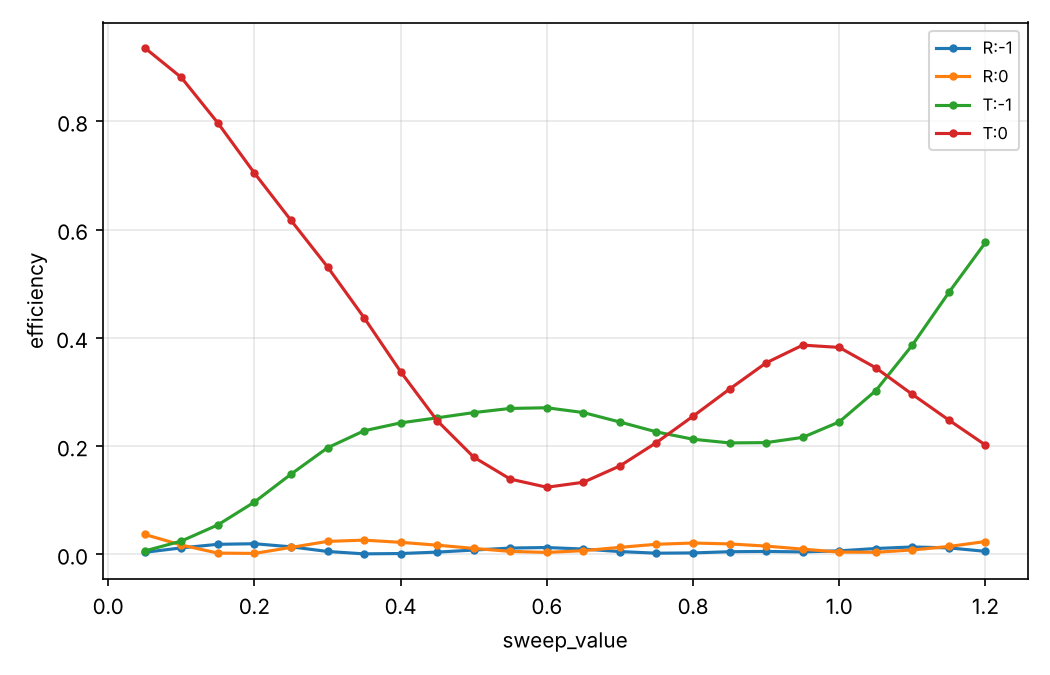
\includegraphics[width=0.78\linewidth]{fig/sweep_te.png}
\caption{Effizienzen über der Stegtiefe (TE). Die nullte Transmissionsordnung wird bei etwa 0,6\um{} Tiefe
weitgehend unterdrückt; dort geht die Leistung in die Ordnung $-1$.}
\end{figure}

\section{Darstellung mit \texttt{plot\_efficiencies.py}}
\begin{lstlisting}[style=shell]
scripts/plot_efficiencies.py CSV [--x SPALTE] [--orders R:0 T:-1 ...] [--quantity efficiency|eff_s|eff_p]
                                 [--lambda W] [--phi W] [--psi W] [--delta W] [--out bild.png]
\end{lstlisting}
\begin{itemize}
  \item Die $x$-Achse ist die erste veränderliche Spalte aus \texttt{sweep\_value}, \texttt{lambda\_um},
        \texttt{phi\_deg}, \texttt{psi\_deg}, \texttt{delta\_deg} oder die mit \texttt{-{}-x} gewählte.
  \item \texttt{-{}-orders} wählt Ordnungen als \texttt{Seite:n} oder \texttt{Seite:n:m}; ohne Angabe alle.
  \item Die übrigen veränderlichen Spalten halten Sie mit \texttt{-{}-lambda}, \texttt{-{}-phi}, \texttt{-{}-psi},
        \texttt{-{}-delta} fest.
  \item Ohne \texttt{-{}-out} öffnet sich ein Fenster.
\end{itemize}

\chapter{Nahfeld}\label{ch:nahfeld}
\index{Nahfeld}%

Neben den Effizienzen berechnet \FG{} die Felder $\mathbf E$ und $\mathbf H$ in der Struktur und in ihrer Umgebung.
Das zeigt Feldüberhöhungen, Resonanzen, Moden und Absorptionsorte.

\section{Schnitte}
\begin{center}
\begin{tikzpicture}[scale=1.4]
  % 3D-artige Zelle
  \draw[fill=gray!20] (0,0) -- (3,0) -- (3.8,0.6) -- (0.8,0.6) -- cycle;
  \draw[fill=blue!25] (0,0) -- (3,0) -- (3,1.2) -- (0,1.2) -- cycle;
  \draw[fill=blue!15] (3,0) -- (3.8,0.6) -- (3.8,1.8) -- (3,1.2) -- cycle;
  \draw[fill=blue!8] (0,1.2) -- (3,1.2) -- (3.8,1.8) -- (0.8,1.8) -- cycle;
  % vertikaler Schnitt
  \draw[very thick,red!70!black,fill=red!15,opacity=0.7] (0.4,-0.6) -- (3.4,-0.6) -- (3.4,2.4) -- (0.4,2.4) -- cycle;
  \node[red!70!black,anchor=west] at (3.5,2.2) {\small vertikaler Schnitt: $z=z_0$, Karte $(x,y)$};
  % horizontaler Schnitt
  \draw[very thick,fgblue,fill=fgblue!15,opacity=0.7] (-0.3,0.7) -- (3.0,0.7) -- (4.1,1.5) -- (0.8,1.5) -- cycle;
  \node[fgblue,anchor=west] at (4.2,1.1) {\small horizontaler Schnitt: $y=y_0$};
  \node[fgblue,anchor=west] at (4.2,0.75) {\small 1D: Linie $u(x)$; 2D: Karte $(x,z)$};
  \draw[->] (-0.8,-0.4) -- (-0.3,-0.4) node[right] {\scriptsize$x$};
  \draw[->] (-0.8,-0.4) -- (-0.8,0.1) node[above] {\scriptsize$y$};
  \draw[->] (-0.8,-0.4) -- (-0.5,-0.2) node[above right] {\scriptsize$z$};
\end{tikzpicture}
\end{center}
Je Rechnung gibt es zwei Schnitte:
\begin{itemize}
  \item den \textbf{vertikalen Schnitt} bei $z=z_0$: eine Karte über $x$ und $y$ (bei 1D-Gittern spielt $z_0$ keine Rolle),
  \item den \textbf{horizontalen Schnitt} bei $y=y_0$: bei 1D-Gittern eine Linie über $x$, bei 2D-Gittern eine Karte über
        $x$ und $z$.
\end{itemize}

\section{Konfiguration}
\begin{lstlisting}[language=json]
"nearfield": {
  "enabled": true,
  "horizontal_y_um": 0.125,      // Lage y0 des horizontalen Schnitts
  "vertical_z_um": 0.0,          // Lage z0 des vertikalen Schnitts
  "y_range_um": [-0.3, 0.6],     // y-Bereich des vertikalen Schnitts
  "nx": 400, "ny": 360, "nz": 200,
  "periods": 2,                  // Zahl der dargestellten Perioden
  "reconstruction": "fff",       // "fff" oder "direct"
  "field": "total"               // "total" oder "scattered" (isolierte Strukturen)
}
\end{lstlisting}
\begin{center}
\small
\begin{tabularx}{\linewidth}{lllY}
\toprule
Schlüssel & Typ & Standard & Bedeutung \\
\midrule
\key{enabled} & bool & \val{false} & Nahfeld berechnen \\
\key{horizontal\_y\_um} & Zahl & 0 & $y_0$ (im Substrat negativ) \\
\key{vertical\_z\_um} & Zahl & 0 & $z_0$ (nur 2D wirksam) \\
\key{y\_range\_um} & Liste & $[-0{,}2;\,0{,}5]$ & $y$-Bereich der vertikalen Karte \\
\key{nx}, \key{ny}, \key{nz} & Zahl & 400, 300, 200 & Punkte je Achse (über alle dargestellten Perioden) \\
\key{periods} & Zahl & 1 & Perioden in $x$ (und $z$) \\
\key{reconstruction} & Text & \val{"fff"} & Rekonstruktion der Felder (siehe unten) \\
\key{field} & Text & \val{"total"} & \val{scattered}: nur das Streufeld (Abschnitt~\ref{sec:pml}) \\
\key{quantities} & Liste & & Wunschliste der Größen; geschrieben werden derzeit stets alle \\
\bottomrule
\end{tabularx}
\end{center}
Das Nahfeld wird für den \textbf{ersten Scanpunkt} berechnet (bei Sweeps: des ersten Sweep-Werts). Für mehrere
Wellenlängen rechnen Sie mehrere Konfigurationen oder nutzen Python.

\section{Rekonstruktion: \texttt{fff} oder \texttt{direct}}
\index{Nahfeld!Rekonstruktion}%
An einer Materialgrenze springt die Normalkomponente von $\mathbf E$; stetig ist $\mathbf D_\perp=\varepsilon
\mathbf E_\perp$. Eine abgeschnittene Fourierreihe kann einen Sprung nur mit Gibbs-Schwingungen darstellen.
\begin{description}
  \item[\val{fff}] (Standard) rekonstruiert die stetigen Größen (tangentiales $\mathbf E$, normales $\mathbf D$)
        und berechnet daraus $\mathbf E$. Die Felder sind an Grenzen glatt und physikalisch richtig.
  \item[\val{direct}] summiert die Fourierreihe von $\mathbf E$ direkt. An Wänden entstehen Überschwinger (beim Sprung
        von $D_x$ an Lamellenwänden etwa 300\,\%). Nur für Vergleiche.
\end{description}

\section{Ausgabedateien}\label{sec:nf-dateien}
\cmd{fgsolve} schreibt je Schnitt ein Verzeichnis \file{nearfield\_vertical/} bzw.\ \file{nearfield\_horizontal/} in
\key{output.dir}:
\begin{center}
\small
\begin{tabularx}{\linewidth}{llY}
\toprule
Datei & Typ & Inhalt \\
\midrule
\file{Ex.npy} \ldots{} \file{Ez.npy} & complex128 & elektrisches Feld, bezogen auf $|\mathbf E_{\text{inc}}|=1$ \\
\file{Hx.npy} \ldots{} \file{Hz.npy} & complex128 & magnetisches Feld als $Z_0\mathbf H$ (gleiche Größenordnung wie $\mathbf E$) \\
\file{absE2.npy}, \file{absH2.npy} & float64 & $|\mathbf E|^2$, $|Z_0\mathbf H|^2$ \\
\file{Sy.npy} & float64 & $S_y=\tfrac12\operatorname{Re}(\mathbf E\times\mathbf H^*)_y$ (negativ = abwärts) \\
\file{material.npy} & float64 & $\operatorname{Re}\varepsilon$ in jedem Punkt (zeigt die Geometrie) \\
\file{meta.json} & JSON & Achsen (\texttt{axis1}, \texttt{axis2} mit Werten in \textmu m), Schnitt, $\lambda$, Normierung \\
\bottomrule
\end{tabularx}
\end{center}
Karten haben die Form \texttt{(len(axis2), len(axis1))} in C-Reihenfolge, Linien die Form \texttt{(len(axis1),)}.
Beim vertikalen Schnitt ist \texttt{axis1} $=x$ und \texttt{axis2} $=y$.

\textbf{Mit numpy laden.}
\begin{lstlisting}[style=py]
import json, numpy as np
d = "out/nearfield_lamellar_1d/nearfield_vertical"
meta = json.load(open(f"{d}/meta.json"))
x = np.array(meta["axes"]["axis1"]["values_um"])
y = np.array(meta["axes"]["axis2"]["values_um"])
E2 = np.load(f"{d}/absE2.npy")            # Form (len(y), len(x))
eps = np.load(f"{d}/material.npy")
print("max |E|^2 =", E2.max(), "bei y =", y[np.unravel_index(E2.argmax(), E2.shape)[0]])
\end{lstlisting}

\section{Darstellung mit \texttt{plot\_nearfield.py}}
\begin{lstlisting}[style=shell]
scripts/plot_nearfield.py out/nearfield_lamellar_1d/nearfield_vertical --quantity absE2 --out e2.png
scripts/plot_nearfield.py DIR --quantity Ex --part re|im|abs|phase
\end{lstlisting}
Das Skript zeichnet die Materialgrenzen aus \file{material.npy} als weiße Linien ein.

\begin{figure}[h]
\centering
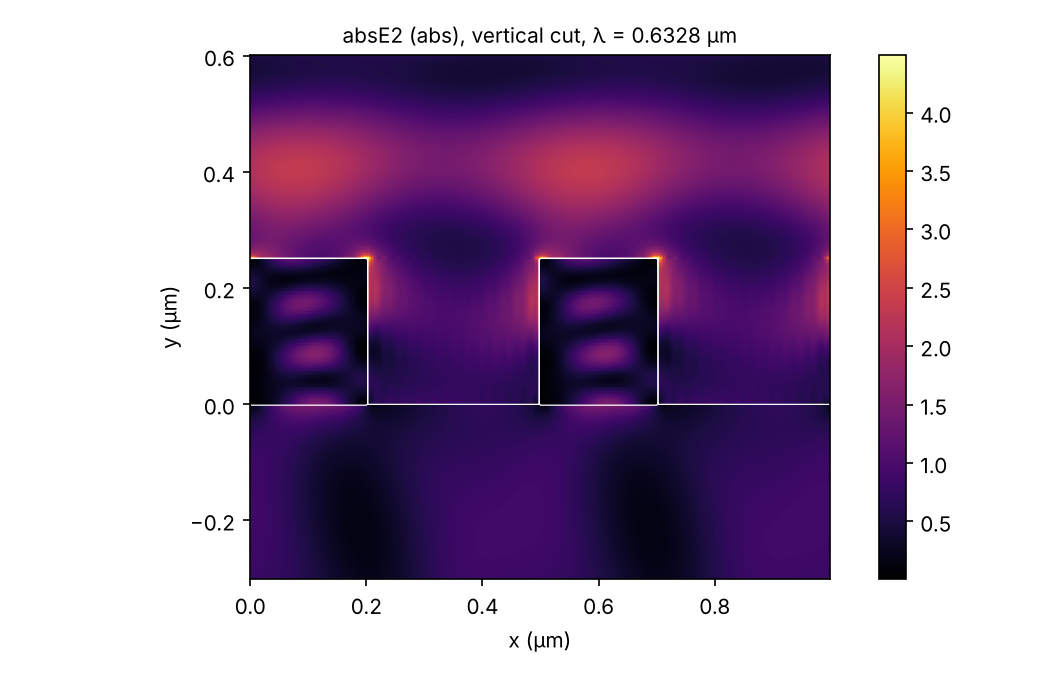
\includegraphics[width=0.68\linewidth]{fig/nf1d_vertical.png}
\caption{$|\mathbf E|^2$ im vertikalen Schnitt durch Siliziumlamellen auf Glas (\file{examples/nearfield\_lamellar\_1d.json},
TM, $\lambda=0{,}6328$\um, zwei Perioden). An den oberen Kanten der Stege ist das Feld stark überhöht; im Silizium
bildet sich eine Stehwelle.}
\end{figure}

\begin{figure}[h]
\centering
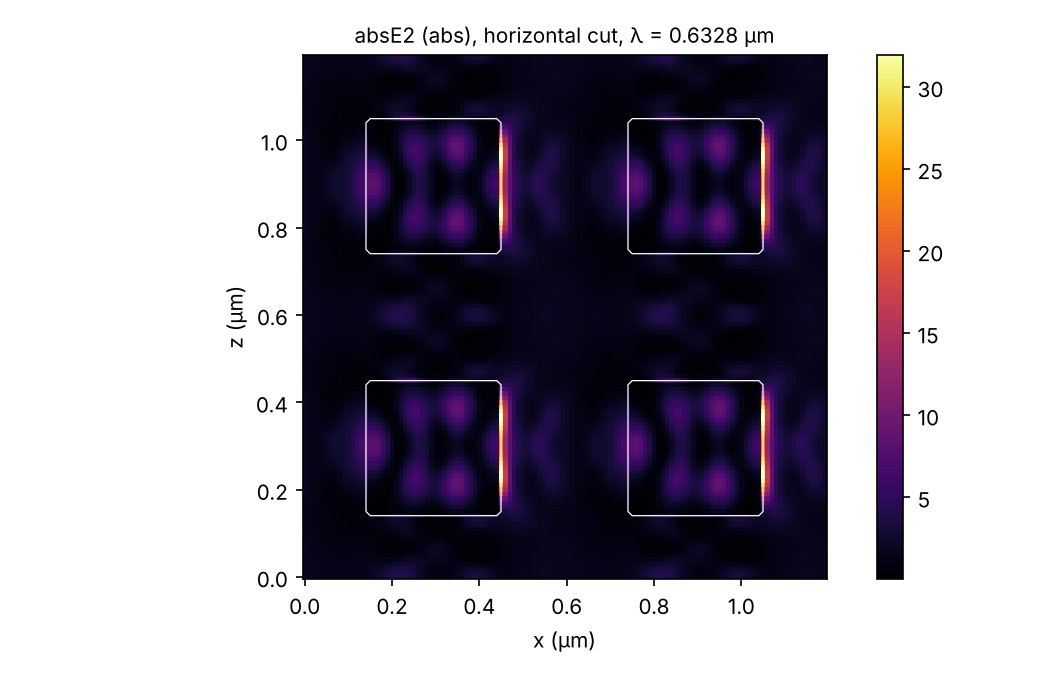
\includegraphics[width=0.6\linewidth]{fig/nf2d_horizontal.png}
\caption{Horizontaler Schnitt durch quadratische Siliziumsäulen (\file{examples/nearfield\_pillars\_2d.json}) in
halber Höhe, $|\mathbf E|^2$ über $x$ und $z$.}
\end{figure}

\section{Nahfeld in Python}
\begin{lstlisting}[style=py]
nf = fg.near_field(cfg)                      # Block "nearfield" der Konfiguration
v = nf["vertical"]
v["absE2"], v["Ex"], v["axis1_um"], v["axis2_um"], v["material"], v["meta"]
\end{lstlisting}
Die Arrays sind identisch mit den \file{.npy}-Dateien von \cmd{fgsolve}.

\section{Hinweise}
\begin{itemize}
  \item Die Auflösung \key{nx}, \key{ny} kostet kaum Rechenzeit; teuer ist die Rechnung selbst. Für Resonanzen
        lohnt sich ein höheres $N$ als für Effizienzen, weil lokale Feldspitzen langsamer konvergieren.
  \item Bei RCWA-Profilen ist das Feld innerhalb der Treppe die Lösung der Treppe, nicht des glatten Profils.
  \item Bei Metallen liegt das Feldmaximum oft an Kanten; dort konvergiert das Feld am langsamsten.
\end{itemize}

\chapter{Ausgaben und Diagnose}\label{ch:ausgabe}

\section{Terminalausgabe von \texttt{fgsolve}}
Für jeden Scanpunkt erscheint ein Block:
\begin{lstlisting}
lambda = 0.6328 um, phi = 10 deg, psi = 0 deg, delta = 90 deg
  side   n    m   efficiency
  R     -1    0   0.2329942258
  R      0    0   0.0901052774
  T     -1   -1   0.0698534457
  ...
  sum R+T = 0.789794795102   absorption = 2.102e-01
\end{lstlisting}
Darunter stehen gegebenenfalls
\begin{itemize}
  \item \texttt{precision fp32 (repeated in fp64)} -- die tatsächlich verwendete Genauigkeit, wenn nicht fp64,
  \item \texttt{warning: \ldots} -- Warnungen (z.\,B.\ \val{FFF\_iso} bei einem Metall),
  \item bei isolierten Strukturen \texttt{scattered up = \ldots{} down = \ldots{} absorbed = \ldots} statt der
        Ordnungen,
  \item bei Modenanregung die Zeilen \texttt{MR}, \texttt{MT} mit effektivem Index und Leistung je Mode,
  \item bei Sweeps vor jedem Wert die Zeile \texttt{== sweep <pointer> = <wert>},
  \item bei dispersiven Materialien je Material und Scanpunkt die ausgewerteten Werte, bei \key{eps\_principal}
        je Hauptachse mit \texttt{[1]}--\texttt{[3]}:
\begin{lstlisting}
  material ag: n = 0.1578809+1.8273612i   eps = -3.3143227+0.57701088i
\end{lstlisting}
\end{itemize}
Am Ende nennt \cmd{fgsolve} die geschriebenen Dateien.

\section{\texttt{efficiencies.csv}}\label{sec:csv}
\index{efficiencies.csv@\file{efficiencies.csv}}%
Eine Zeile je Ordnung und Scanpunkt, Komma als Trennzeichen, Punkt als Dezimalzeichen.
\begin{center}
\small
\begin{tabularx}{\linewidth}{lY}
\toprule
Spalte & Bedeutung \\
\midrule
\texttt{sweep\_parameter}, \texttt{sweep\_value} & nur bei Sweeps: Pointer und Wert \\
\texttt{lambda\_um}, \texttt{phi\_deg}, \texttt{psi\_deg}, \texttt{delta\_deg} & Scanpunkt \\
\texttt{side} & \texttt{R} (reflektiert) oder \texttt{T} (transmittiert); Sonderfälle siehe unten \\
\texttt{n}, \texttt{m} & Ordnung (in 1D ist \texttt{m} $=0$) \\
\texttt{efficiency} & Beugungseffizienz \\
\texttt{eff\_s}, \texttt{eff\_p} & s- und p-Anteil (nur bei isotropen Halbräumen, sonst 0) \\
\texttt{amp\_s\_re}, \texttt{amp\_s\_im}, \texttt{amp\_p\_re}, \texttt{amp\_p\_im} & komplexe Amplituden der
s- und p-Komponente \\
\bottomrule
\end{tabularx}
\end{center}
Sonderwerte von \texttt{side}:
\begin{center}
\small
\begin{tabularx}{\linewidth}{lY}
\toprule
\texttt{side} & Bedeutung \\
\midrule
\texttt{S\_up}, \texttt{S\_down}, \texttt{S\_abs} & isolierte Strukturen: Streuleistung nach oben, nach unten, Absorption
(1D: Streubreite in \textmu m, 2D: Streuquerschnitt in \textmu m$^2$) \\
\texttt{MR}, \texttt{MT}, \texttt{Mrad} & Modenanregung: reflektierte und transmittierte Modenleistung (\texttt{n} =
Modennummer), abgestrahlte Leistung \\
\texttt{C\_R}, \texttt{C\_T}, \texttt{C\_A} & Zylinder, Strahl: Reflexion, Transmission, Rest (bezogen auf den
einfallenden Strahl) \\
\texttt{C\_Rm}, \texttt{C\_Tm} & Zylinder: Anteil je azimutaler Harmonischer (\texttt{n} $=m$) \\
\texttt{C\_Sup}, \texttt{C\_Sdown}, \texttt{C\_Ssca} & Zylinder, ebene Welle: Streuquerschnitte in \textmu m$^2$ \\
\bottomrule
\end{tabularx}
\end{center}

\textbf{Einlesen.}
\begin{lstlisting}[style=py]
import pandas as pd
df = pd.read_csv("out/v3/efficiencies.csv")
t1 = df[(df.side == "T") & (df.n == 1)]
print(t1[["lambda_um", "efficiency"]])
\end{lstlisting}

\section{\texttt{materials.csv}}\label{sec:materials-csv}
\index{materials.csv@\file{materials.csv}}%
Mit \val{"output": \{"materials": "materials.csv"\}} schreibt \cmd{fgsolve} die Materialwerte je
Scan-Wellenlänge, auch die der festen Materialien (ohne \key{eps\_tensor}):
\begin{lstlisting}
lambda_um,material,component,n_re,n_im,eps_re,eps_im
0.4,ag,iso,0.15788090118,1.82736122912,-3.31432268272,0.577010875269
0.4,air,iso,1,0,1,0
\end{lstlisting}
\texttt{component} ist \val{iso} oder bei \key{eps\_principal} die Hauptachse \val{1}--\val{3}. So lässt sich
nachprüfen, mit welchen Werten tatsächlich gerechnet wurde.

\section{Diagnose}\label{sec:diagnose}
\index{Diagnose}%
\begin{center}
\small
\begin{tabularx}{\linewidth}{lY}
\toprule
Größe (Python: \texttt{res.diagnostics[...]}) & Bedeutung, Bewertung \\
\midrule
\texttt{energy\_balance} & $\sum R + \sum T$; bei verlustfreien Strukturen 1 \\
\texttt{max\_condition\_t11} & größte Konditionszahl der Teilblöcke bei der S-Matrix-Verkettung; sehr große Werte
($>10^{12}$) deuten auf numerische Probleme \\
\texttt{rk\_steps} & Zahl der Runge--Kutta-Schritte \\
\texttt{warnings} & Liste von Warnungen (auch: Tabelle außerhalb ihres Bereichs mit \val{"extrapolate":
"constant"}) \\
\texttt{materials} & dispersive Materialien am Scanpunkt: Liste mit \texttt{name}, \texttt{component} (0 isotrop,
1--3 Hauptachse), \texttt{n}, \texttt{eps} \\
\texttt{precision} & tatsächlich verwendete Genauigkeit (\val{fp64}, \val{mixed}, \val{fp32}) \\
\texttt{precision\_fallback} & \val{true}, wenn eine fp32-Rechnung in fp64 wiederholt wurde \\
\texttt{refinement\_steps}, \texttt{refinement\_fallbacks} & Nachiterationen bei \val{mixed} \\
\texttt{timings} & \texttt{solve\_s} und bei \texttt{profile=True} die Zeit je Abschnitt \\
\bottomrule
\end{tabularx}
\end{center}

\section{Profil der Rechenzeit}
\index{Profil der Rechenzeit}%
\begin{lstlisting}[style=shell]
$ fgsolve --profile examples/nearfield_pillars_2d.json
...
profile (busy time summed over threads):
  wall                           1.5766 s         1 x  max 1.5766 s
  nearfield                      1.0279 s         1 x  max 1.0279 s
  nearfield.coefficients         0.8220 s         1 x  max 0.8220 s
  solve.assemble                 0.5543 s         2 x  max 0.2948 s
  solve.layer_models             0.3919 s         2 x  max 0.2352 s
  linalg.eig                     0.1728 s         2 x  max 0.0990 s
  ...
written: out/nearfield_pillars_2d/profile.json
\end{lstlisting}
Die Zeiten sind über alle Threads summiert. Typische Abschnitte: \texttt{linalg.eig} (Eigenwertprobleme der RCWA),
\texttt{smatrix.star} (Verkettung), \texttt{nf.raster}/\texttt{nf.coefficients} (Normalenfeld),
\texttt{nearfield.*} (Nahfeld). In Python: \texttt{fg.solve(cfg, profile=True).diagnostics["timings"]["scopes"]}.

\section{Rückgabewerte von \texttt{fgsolve}}
\index{Rückgabecode}%
\begin{center}
\small
\begin{tabular}{cl}
\toprule
Code & Bedeutung \\
\midrule
0 & Erfolg \\
1 & ohne Argument aufgerufen (Kurzhilfe) \\
2 & Funktion noch nicht umgesetzt (\texttt{NotImplemented}) \\
3 & Fehler in Konfiguration oder Rechnung (\texttt{fgsolve: error: \ldots}) \\
4 & \texttt{-{}-cad-report}: Befunde mit Fehlern \\
\bottomrule
\end{tabular}
\end{center}
In Skripten lässt sich so zuverlässig prüfen, ob eine Rechnung gelaufen ist.

\chapter{Erweiterte Funktionen}\label{ch:erweitert}

\section{Adaptive räumliche Auflösung (ASR)}\label{sec:asr}
\index{ASR}\index{Koordinatentransformation}%
Bei Metallstrukturen in TM konzentriert sich das Feld an den Kanten; dort braucht die Fourierreihe die meisten
Ordnungen. Die adaptive räumliche Auflösung nach Granet verzerrt die Koordinate $x$ (und $z$) so, dass die
Fourierbasis an den Materialsprüngen feiner auflöst. Die Zahl der Ordnungen bleibt gleich, die Konvergenz wird
deutlich schneller.
\begin{lstlisting}[language=json]
"coordinate_transform": {
  "x": { "type": "asr", "eta": 0.9, "breakpoints_um": "auto" },
  "z": { "type": "asr", "eta": 0.5, "breakpoints_um": [0.1, 0.4] }     // nur 2D
}
\end{lstlisting}
\begin{center}
\small
\begin{tabularx}{\linewidth}{llY}
\toprule
Schlüssel & Standard & Bedeutung \\
\midrule
\key{type} & -- & \val{"asr"} \\
\key{eta} & 0 & Verdichtung $0\le\eta<1$; das Raster wird an den Stellen um den Faktor $1-\eta$ feiner. $\eta=0$ ist
keine Transformation (bitgleich zur Rechnung ohne Block) \\
\key{breakpoints\_um} & \val{"auto"} & Stellen der Verdichtung: \val{"auto"} nimmt alle Materialsprünge der
Lamellenschichten und die Eckkoordinaten der Polygone; oder eine Liste \\
\bottomrule
\end{tabularx}
\end{center}
\begin{itemize}
  \item Empfehlung für Metall-Lamellen in TM: $\eta=0{,}8$ bis $0{,}95$. Das Beispiel in
        Abschnitt~\ref{sec:konvergenz} zeigt: Mit $\eta=0{,}95$ ist $e_{-1}$ eines Goldgitters ab $N=20$ auf vier Stellen
        genau, ohne ASR auch bei $N=80$ nicht.
  \item Bei Profilschichten gibt es keine Sprünge, die \val{"auto"} finden könnte; geben Sie dann eine Liste an,
        sonst meldet \FG{} \texttt{no material jumps found along the axis, give breakpoints\_um}.
  \item Mit einer einzigen Stelle ist die Abbildung analytisch (schnellste Konvergenz). Bei mehreren ungleich langen
        Intervallen konvergiert die Rechnung algebraisch ($\sim N^{-5}$).
  \item Mit ASR wird \key{split\_polarizations} nicht genutzt; ASR und PML schließen sich aus.
  \item Im Nahfeld bleibt die Ausgabe auf dem physikalischen Raster; nur die Fourierkoeffizienten
        (\texttt{fieldCoefficients}) beziehen sich auf die transformierten Koordinaten.
\end{itemize}

%-------------------------------------------------------------------------------------------
\section{Isolierte Strukturen mit PML}\label{sec:pml}
\index{PML}\index{isolierte Struktur}\index{Streufeld}%
Ein einzelner Steg, ein Graben, ein Kontaktloch oder ein Wellenleiterende ist nicht periodisch. \FG{} rechnet ihn in
einer Rechenzelle mit \textbf{absorbierenden Randzonen} (perfectly matched layers, PML): Am Zellrand wird die
Koordinate komplex gestreckt, sodass auslaufende Wellen dort ohne Reflexion abklingen. Die Nachbarzellen sehen sich
dann nicht mehr.
\begin{center}
\begin{tikzpicture}[scale=1.4]
  \fill[gray!25] (0,-0.6) rectangle (6,0);
  \fill[red!12] (0,-0.6) rectangle (1,1.4);
  \fill[red!12] (5,-0.6) rectangle (6,1.4);
  \fill[blue!50] (2.8,0) rectangle (3.2,0.4);
  \draw (0,-0.6) rectangle (6,1.4);
  \draw[dashed] (1,-0.6) -- (1,1.4); \draw[dashed] (5,-0.6) -- (5,1.4);
  \node at (0.5,1.15) {\small PML}; \node at (5.5,1.15) {\small PML};
  \node at (3,1.15) {\small physikalischer Bereich $[w,\,d-w]$};
  \draw[<->] (0,-0.75) -- (1,-0.75) node[midway,below] {\small $w$};
  \draw[<->] (0,-1.15) -- (6,-1.15) node[midway,below] {\small Zellbreite $d$ = \key{period\_um.x}};
\end{tikzpicture}
\end{center}
\begin{lstlisting}[language=json]
"aperiodic": {
  "pml": { "x": { "width_um": 0.8, "beta": 1.0 },
           "z": { "width_um": 0.8 } },       // z nur in 2D
  "formulation": "auto",                     // oder "scattered"
  "excitation": "plane_wave"                 // oder {"mode": 0} bzw. {"n_eff": 1.9}
}
\end{lstlisting}
\begin{center}
\small
\begin{tabularx}{\linewidth}{llY}
\toprule
Schlüssel & Standard & Bedeutung \\
\midrule
\key{pml.x.width\_um} & -- & Breite $w$ der Randzone an beiden Zellenden \\
\key{pml.x.beta} & 1,0 & Stärke der Absorption \\
\key{formulation} & \val{auto} & \val{auto}: Totalfeld bei Normaleinfall, Streufeld bei schrägem Einfall;
\val{scattered}: immer Streufeld \\
\key{excitation} & \val{plane\_wave} & oder geführte Mode eines strukturierten Superstrats (siehe unten) \\
\bottomrule
\end{tabularx}
\end{center}
\paragraph{Regeln.}
\begin{itemize}
  \item Strukturen dürfen nicht in die PML-Zonen reichen (geprüft, auch für CAD-Schnitte). Durchgehende Filme
        (homogene Schichten) dürfen durchlaufen.
  \item Die Zellbreite muss deutlich größer sein als die Struktur. Bei gleicher Auflösung wächst die nötige
        Ordnungszahl $N$ proportional zur Zellbreite; prüfen Sie Konvergenz in $N$ \emph{und} in der Zellbreite.
  \item PML und ASR schließen sich aus.
\end{itemize}

\paragraph{Ausgabe.} Statt Beugungseffizienzen gibt es Streugrößen, bezogen auf die Intensität der einfallenden
Welle (1D: Streubreite in \textmu m, 2D: Streuquerschnitt in \textmu m$^2$):
\begin{lstlisting}
lambda = 0.6328 um, phi = 0 deg, psi = 0 deg, delta = 0 deg
  side   n    m   efficiency
  scattered up = 0.3289787262   down = 0.3704020556   absorbed = 0.02285324735   (um, 2D: um^2)
\end{lstlisting}
Das ist ein 0,3\um{} breiter Siliziumsteg (0,2\um{} hoch) auf Glas in einer 4\um{} breiten Zelle mit 0,8\um{} PML
($N=60$, Rechenzeit etwa 8\,s). In der CSV-Datei heißen die Zeilen \texttt{S\_up}, \texttt{S\_down},
\texttt{S\_abs}; in Python \texttt{res.scattering} mit den Schlüsseln \texttt{up}, \texttt{down}, \texttt{lateral},
\texttt{absorbed}.
\begin{itemize}
  \item \texttt{up}/\texttt{down}: Leistung des Streufeldes durch die Ebenen oberhalb und unterhalb der Struktur über
        den physikalischen Bereich.
  \item \texttt{lateral}: durch die Seiten der Box; \texttt{absorbed}: in der Box absorbiert.
  \item Nur die Summe \texttt{up + down + lateral} ist unabhängig von der Zellbreite. Die Aufteilung oben/unten
        konvergiert bei schrägem Einfall langsam ($\sim1/L$).
\end{itemize}

\paragraph{Totalfeld und Streufeld.} Bei senkrechtem Einfall rechnet \FG{} das Totalfeld und zieht den
Hintergrund ab (jede strukturierte Schicht ersetzt durch ihr Material am Zellrand). Bei schrägem Einfall wäre die
einfallende Welle nicht periodisch; dann verwendet \FG{} automatisch die \textbf{Streufeldformulierung}: Der
Hintergrund wird analytisch gelöst, die Struktur wirkt als Quelle $\sigma=(M-M_{\text{bg}})F_{\text{bg}}$. Mit
\val{"nearfield": \{"field": "scattered"\}} geben Sie im Nahfeld nur das Streufeld aus.

\subsection{Anregung durch eine geführte Mode}
Ein strukturierter Halbraum (z.\,B.\ ein Wellenleiter, der in $y$-Richtung läuft) kann eine Mode einspeisen; berechnet
werden die Leistungen der reflektierten und transmittierten Moden. Typische Anwendung: Wellenleiterenden,
Taper, Gitterkoppler.
\begin{lstlisting}[language=json]
"aperiodic": { "pml": { "x": { "width_um": 0.5 } }, "excitation": { "mode": 0 } },
"superstrate_structure": { "type": "lamellar1d",
                           "breakpoints_um": [0, 1.3, 1.7, 3.0],
                           "materials": ["air", "core", "air"] },
"substrate_structure": { ... }
\end{lstlisting}
\begin{itemize}
  \item \key{superstrate\_structure}, \key{substrate\_structure}: $y$-invariante Querschnitte (\val{lamellar1d},
        \val{polygon2d}, \val{contour2d}) der Halbräume; die Dicke entfällt. \key{superstrate}/\key{substrate} nennen dann
        den Mantel.
  \item \key{excitation}: \val{\{"mode": k\}} wählt die $k$-te geführte Mode nach absteigendem effektivem Index,
        \val{\{"n\_eff": x\}} die Mode mit dem nächstgelegenen Index.
  \item Ausgabe: \texttt{MR}/\texttt{MT} je Mode (Modennummer und Leistung), \texttt{Mrad} (abgestrahlt); Python
        \texttt{res.modal}.
\end{itemize}

\subsection{Streufeldformulierung für periodische Gitter}
\val{"scattered\_field": true} erzwingt die Streufeldformulierung auch bei periodischen Gittern. Die Effizienzen sind
dann die von Hintergrund plus Streufeld; das Ergebnis ist dasselbe wie ohne. Gedacht ist die Option für Tests
(Referenzfall V20d).

%-------------------------------------------------------------------------------------------
\section{Rotationssymmetrische Strukturen (in Arbeit)}\label{sec:zylinder}
\index{Zylinderkoordinaten}\index{Gauß-Strahl}%
Säulen, Scheiben, Löcher, Ringe und Zonenplatten auf einem Schichtstapel sind rotationssymmetrisch um eine Achse
senkrecht zum Stapel. In Zylinderkoordinaten entkoppeln die azimutalen Harmonischen $e^{im\varphi}$; je Harmonischer
bleibt ein Problem in $(r,y)$. Das ist viel günstiger, als die isolierte Struktur kartesisch mit PML zu rechnen.

\begin{achtung}[Stand]
Meilenstein M20 ist teilweise umgesetzt: Schichttypen \val{homogeneous}, \val{rings} und \val{rings\_profile},
isotrope Materialien, Gauß-Strahlen auf der Achse und ebene Wellen (Streufeld), Leistungen, Streu-, Absorptions- und
Extinktionsquerschnitt, Nahfeld, Winkelspektrum und Fernfeld, CAD-Rotationskörper
(Abschnitt~\ref{sec:cad-axisym-hb}).
\end{achtung}

\begin{lstlisting}[language=json]
{
  "cylindrical": {
    "symmetry": "axial",
    "harmonics": "auto",                                   // oder Liste, z. B. [-1, 1]
    "spectrum": { "kappa_max": 4, "dk_factor": 1.0, "deform": "auto" },
    "factorization": "li_r"                                // oder "laurent"
  },
  "solver": "rcwa",
  "materials": { "air": {"n": 1.0}, "glass": {"n": 1.5}, "sin": {"n": 1.45} },
  "superstrate": "air", "substrate": "glass",
  "incidence": { "type": "gaussian_beam", "lambda_um": [0.9, 1.0, 1.1],
                 "waist_um": 0.5, "focus_y_um": 0.8, "polarization": "x" },
  "layers": [ { "type": "rings", "thickness_um": 0.3, "radii_um": [0.4],
                "materials": ["sin", "air"] } ],
  "output": { "dir": "out_cyl_pillar_beam" }
}
\end{lstlisting}
\begin{center}
\small
\begin{tabularx}{\linewidth}{llY}
\toprule
Schlüssel & Standard & Bedeutung \\
\midrule
\key{symmetry} & \val{axial} & Rotationssymmetrie ($P$-zählige Symmetrie folgt mit M21) \\
\key{harmonics} & \val{auto} & azimutale Ordnungen $m$; \val{auto}: $m=\pm1$ bei Strahl/Normaleinfall, sonst
$|m|\le m_{\text{cut}}$ \\
\key{spectrum.kappa\_max} & & obere Grenze des Hankel-Spektrums (in Einheiten von $k_0$) -- der Genauigkeitsparameter \\
\key{spectrum.dk\_factor} & 1,0 & Feinheit der Stützstellen; um Plasmonen eines Metallfilms zwischen verschiedenen Halbräumen wird automatisch verfeinert \\
\key{spectrum.nodes\_per\_panel} & 8 & Gauß-Knoten je Teilintervall \\
\key{spectrum.deform} & \val{auto} & komplexer Integrationsweg um Verzweigungspunkte: \val{auto}, \val{false} oder
\val{\{"delta": 0.05\}} \\
\key{factorization} & \val{li\_r} & \val{li\_r} (Li-Regel in $r$) oder \val{laurent} \\
\key{optical\_theorem} & \val{false} & ebene Welle: optisches Theorem als Kontrolle (\texttt{C\_Sext\_ot}); kostet
etwa die doppelte Rechenzeit, bei verlustbehafteten Ringen ohnehin berechnet \\
\key{far\_field.n\_phi} & -- & Fernfeld auf so vielen Azimuten, dazu \texttt{angular\_spectrum.csv} und
\texttt{far\_field.csv} \\
\bottomrule
\end{tabularx}
\end{center}
\paragraph{Schichten mit veränderlichem Radius.} \val{rings\_profile} beschreibt Kegelstümpfe, Kugeln, Kugelkappen
und beliebige Rotationsprofile: Jeder Radius ist eine Zahl, \val{\{"cone": [r0, r1]\}} (unten, oben),
\val{\{"sphere": \{"center\_y\_um": c, "radius\_um": R\}\}} ($y$ ab der Schichtunterkante) oder eine Tabelle
\val{\{"table": \{"y\_um": [...], "r\_um": [...]\}\}}. Gerechnet wird eine Treppe aus \key{slices} Scheiben mit den
Radien in der Scheibenmitte; der Treppenfehler fällt etwa mit $1/K^2$, prüfen Sie die Konvergenz in \key{slices}.
\begin{lstlisting}[language=json]
{ "type": "rings_profile", "thickness_um": 0.6, "slices": 20,
  "radii": [ { "sphere": { "center_y_um": 0.3, "radius_um": 0.3 } } ],
  "materials": ["sin", "air"] }
\end{lstlisting}
\paragraph{Einfall.}
\begin{itemize}
  \item \val{gaussian\_beam}: \key{lambda\_um}, \key{waist\_um} (Strahltaille), \key{focus\_y\_um} (Lage des Fokus),
        \key{polarization}: \val{x}, \val{z}, \val{circular\_plus}, \val{circular\_minus}, \val{radial},
        \val{azimuthal}. Winkel sind nicht erlaubt (Strahl auf der Achse).
  \item \val{plane\_wave}: Winkel wie beim kartesischen Einfall, Polarisation über \key{delta\_deg}; Strahlparameter
        sind nicht erlaubt. Gerechnet wird in der Streufeldformulierung.
\end{itemize}
\paragraph{Ausgabe.} Mit dem Beispiel oben:
\begin{lstlisting}
lambda_um,...,side,n,m,efficiency,...
0.9,...,C_R,0,0,0.0474282286936,...
0.9,...,C_T,0,0,0.952447477038,...
0.9,...,C_A,0,0,0.000124294268031,...
0.9,...,C_Rm,-1,0,0.0237141143468,...
0.9,...,C_Tm,-1,0,0.476223738519,...
\end{lstlisting}
\texttt{C\_R}, \texttt{C\_T} sind die reflektierte und transmittierte Leistung relativ zum Strahl, \texttt{C\_A}
$=1-R-T$ (enthält auch den seitlichen Abfluss in geführte Moden). \texttt{C\_Rm}, \texttt{C\_Tm} zerlegen nach
Harmonischen. Bei der ebenen Welle stehen Streuquerschnitte in \textmu m$^2$ in \texttt{C\_Sup}, \texttt{C\_Sdown},
\texttt{C\_Ssca}, dazu der Absorptionsquerschnitt \texttt{C\_Sabs} ($\tfrac1{2I_{\text{inc}}}\int\operatorname{Im}\varepsilon
|\mathbf E|^2\,dV$ über die Ringe), \texttt{C\_Sext} $=$ \texttt{C\_Ssca} $+$ \texttt{C\_Sabs} und zur Kontrolle
\texttt{C\_Sext\_ot} (optisches Theorem; mit \key{optical\_theorem} oder verlustbehafteten Ringen, nicht bei
absorbierendem Hintergrund). Weicht \texttt{C\_Sext\_ot}
deutlich von \texttt{C\_Sext} ab, ist die Rechnung nicht konvergiert. Bei einem Strahl auf verlustbehafteten Ringen
steht in Python \texttt{res.cylindrical["absorbed\_rings"]} die in den Ringen absorbierte Leistung; die Differenz zu
\texttt{C\_A} ist der seitliche Abfluss. Mit \val{"scattered\_field": true} rechnet auch ein Strahl in der
Streufeldformulierung; das Ergebnis ist dasselbe wie beim Totalfeld (eine Kontrolle der Quellen, keine andere Physik).
Python: \texttt{res.cylindrical}. Rechenzeit des Beispiels: etwa 14\,s für
drei Wellenlängen auf zwei Kernen. Konvergenz prüfen Sie über \key{kappa\_max} und \key{dk\_factor}.

\begin{achtung}[Kleine Metallteilchen]
$k_{\max}=\kappa_{\max}\max\operatorname{Re}n$ richtet sich nach dem größten Realteil der Brechzahl. Bei Metallen
($\operatorname{Re}n<1$) und Teilchen, die klein gegen die Wellenlänge sind, braucht es deshalb ein großes
\key{kappa\_max}: $k_{\max}R$ sollte mindestens 15 sein ($R$: Teilchenradius in Einheiten von $1/k_0$). Eine Goldkugel
als Treppe aus Scheiben trifft die Extinktion schnell, die Aufteilung in Streuung und Absorption konvergiert langsam
(Abschnitt~\ref{sec:zylinder_nf}).
\end{achtung}

\paragraph{Winkelspektrum und Fernfeld.}
Jede Rechnung liefert in Python \texttt{res.cylindrical["angular\_spectrum"]}: je Harmonischer $m$ und Seite
(\val{up} ins Superstrat, \val{down} ins Substrat, wenn es verlustfrei ist) die abgestrahlte Leistung je Winkel
$dP/d\theta$ an den Stützstellen des Spektrums ($\theta=\arcsin(k/n)$), getrennt nach s (TE) und p (TM), und das
Quadraturgewicht \texttt{weight}; $\sum\texttt{weight}\cdot(s+p)$ ist die Leistung der Harmonischen
(\texttt{C\_Rm}, \texttt{C\_Tm} bzw.\ \texttt{C\_Supm}, \texttt{C\_Sdownm}). Mit
\val{"far\_field": \{"n\_phi": 72\}} im Block \key{cylindrical} kommt das Fernfeld $dP/d\Omega$ auf (Winkel $\theta$)
$\times$ (72 Azimute) hinzu; \texttt{fgsolve} schreibt dann \texttt{angular\_spectrum.csv} und \texttt{far\_field.csv}.
Beim Strahl ist alles auf die einfallende Leistung bezogen, bei der ebenen Welle ist es der differentielle
Streuquerschnitt in \textmu m$^2$ je Steradiant. Eine kleine Kugel trifft die Mie-Lösung auf $0{,}5\,\%$ des
Maximums ($\kappa_{\max}=8$).

\paragraph{Nahfeld.}\label{sec:zylinder_nf}
Der Block \key{nearfield} (Abschnitt~\ref{ch:nahfeld}) gilt auch hier. Der horizontale Schnitt ist eine Karte in $x$
und $z$, der vertikale Schnitt die Ebene $z=$\,\key{vertical\_z\_um} ($z=0$: Schnitt durch die Achse). $x$ und $z$ laufen
symmetrisch über $[-$\key{extent\_um}$,\,$\key{extent\_um}$]$ mit \key{nx} bzw.\ \key{nz} Punkten einschließlich der
Ränder; Standard ist das 1,5-Fache des äußeren Radius $R_s$, \key{periods} entfällt. Strahlen liefern das Totalfeld,
ebene Wellen Total- oder Streufeld (\key{field}). Mit \val{"reconstruction": "fff"} und Li in $r$ ist die
Normalkomponente $D_r$ an den Ringwänden stetig, $E_r$ springt; \val{direct} glättet den Sprung (Gibbs). Jenseits
von etwa $2R_s$ wird die Synthese ungenauer (die Stützstellendichte ist auf $R_s$ abgestimmt).
\begin{lstlisting}[language=json]
"nearfield": { "enabled": true, "horizontal_y_um": 0.15, "vertical_z_um": 0.0,
               "y_range_um": [-0.3, 1.0], "nx": 201, "ny": 131, "nz": 201, "extent_um": 1.0 }
\end{lstlisting}

\chapter{CAD-Import: STEP-Dateien}\label{ch:cad}
\index{CAD}\index{STEP-Datei}%

Komplizierte 3D-Formen (Säulen mit schrägen Wänden, Kugelkappen, Hohlräume, mehrere Materialien) lassen sich als
STEP-Datei vorgeben. \FG{} zerlegt die Körper entlang $y$ in \textbf{Bänder} und erzeugt daraus automatisch
homogene, \val{contour2d}- und $y$-variable Schichten. Voraussetzung ist ein Build mit CAD-Slicer
(Abschnitt~\ref{sec:inst-cad}); \cmd{fgsolve -{}-info} zeigt \texttt{cad slicer : Nurbforge}.

\section{Ablauf}
\begin{center}
\begin{tikzpicture}[node distance=4mm and 6mm,>=Latex,
  box/.style={draw,rounded corners,fill=fggray,align=center,font=\small,minimum height=8mm,text width=2.5cm}]
  \node[box] (a) {STEP-Datei\\(Körper, Namen)};
  \node[box,right=of a] (b) {Einheit, Achsen\\$\to$ FG-Koordinaten};
  \node[box,right=of b] (c) {kritische Höhen\\$\to$ Bänder};
  \node[box,right=of c] (d) {je Band: homogen, Extrusion, $y$-variabel};
  \draw[->] (a) -- (b); \draw[->] (b) -- (c); \draw[->] (c) -- (d);
\end{tikzpicture}
\end{center}
\begin{enumerate}
  \item Die Körper werden mit Nurbforge gelesen; jeder benannte Körper bekommt ein Material.
  \item Einheit und Achsen werden in \FG-Koordinaten (\textmu m, $y$ = Stapelrichtung) umgerechnet.
  \item \textbf{Kritische Höhen} sind Ecken, ebene Flächen senkrecht zu $y$ und Höhenextrema auf Flächen und Kanten.
        Zwischen zwei kritischen Höhen liegt ein Band; es wird nie auf einer kritischen Höhe geschnitten.
  \item Je Band:
  \begin{itemize}
    \item kein Rand $\to$ \val{homogeneous},
    \item alle Wände parallel zu $y$ (Extrusion) $\to$ ein exakter Schnitt in Bandmitte als \val{contour2d},
    \item sonst $y$-variabel: Schnitte bei Bedarf (RCWA-Treppe oder RK), wahlweise interpoliert.
  \end{itemize}
\end{enumerate}
Extrusionen und Rotationskörper um $y$ (Zylinder, Kegel, Kugel, Torus) liefern exakte Schnittkurven; andere Flächen
werden auf $10^{-9}$ der Modellgröße verfolgt.

\section{STEP-Dateien vorbereiten}
\begin{itemize}
  \item In \textbf{Mikrometern} konstruieren und so schreiben (\texttt{unit="um"}).
  \item \textbf{Ein benannter Körper je Material}, z.\,B.\ \texttt{Pillar}, \texttt{Lid}.
  \item Geschlossene, konsistent orientierte Körper (Volumenkörper, keine offenen Flächen).
  \item Nur für \textbf{2D-Gitter} (\key{period\_um}.z $>0$). Eine $z$-invariante Linie, über genau eine $z$-Periode
        extrudiert, berührt ihr periodisches Bild und wird mit \texttt{PERIODIC\_OVERLAP} abgelehnt: Solche Gitter
        beschreibt man als 1D-Gitter (\val{lamellar1d}, \val{profile1d}).
  \item Mit Nurbforge in Python:
\end{itemize}
\begin{lstlisting}[style=py]
import nurbforge as nf
pillar = ...  # nf.Shell, Koordinaten in µm, CAD +Z = Stapelrichtung
nf.write_step("pillars.step", [pillar, lid], unit="um", names=["Pillar", "Lid"])
\end{lstlisting}
\file{scripts/make\_cad\_examples.py} erzeugt so die Beispiele in \file{examples/cad/}.

\section{Konfiguration}
\begin{lstlisting}[language=json]
{ "type": "cad", "file": "cad/pillar_array.step", "unit": "auto",
  "axes": { "y": "+Z", "x": "+X" },
  "y_range_um": [0.0, 0.26], "cell_origin_um": [0.0, -0.5],
  "background": "superstrate",
  "bodies": [ { "name": "Pillar", "material": "si" }, { "index": 1, "material": "sio2" } ],
  "overlap": "error", "periodic_union": false,
  "slicing": { "critical_tol_um": 1e-6, "min_band_um": 1e-5, "rcwa_slices": 40,
               "y_interpolation": "none", "chebyshev_nodes": 16 },
  "factorization": "auto",
  "normal_field": { "method": "tensor", "grid": 512, "sigma": 3 } }
\end{lstlisting}
\begin{center}
\small
\begin{tabularx}{\linewidth}{lY}
\toprule
Schlüssel & Bedeutung \\
\midrule
\key{file} & STEP-Datei, relativ zur Konfigurationsdatei; alternativ \key{step} mit dem Dateiinhalt als Text \\
\key{unit} & \val{auto}: wie in der Datei deklariert; \val{mm} oder \val{um} erzwingen (korrigiert falsche
Deklarationen) \\
\key{axes} & CAD-Achsen für FG-$y$ (Stapelrichtung) und FG-$x$; FG-$z=x\times y$. Gespiegelte (linkshändige) Achsen
sind verboten, weil sie chirale Strukturen verfälschen \\
\key{y\_range\_um} & $y$-Bereich (Standard: Hüllquader der getrimmten Körper) \\
\key{cell\_origin\_um} & $(x_0,z_0)$ der Zelle in FG-Koordinaten (Standard: Minimum des Hüllquaders); Körper dürfen
über die Zelle ragen \\
\key{background} & Material außerhalb der Körper: Name, \val{superstrate} oder \val{substrate} \\
\key{bodies} & Zuordnung Körper $\to$ Material über den Namen (\key{name}) oder die Position (\key{index});
nicht zugeordnete Körper sind ein Fehler \\
\key{overlap} & \val{error} (Standard) oder \val{priority}: frühere Körper gewinnen \\
\key{periodic\_union} & Körper vor dem Schneiden mit ihren überlappenden periodischen Bildern vereinigen \\
\key{slicing.critical\_tol\_um} & nähere kritische Höhen werden zusammengelegt \\
\key{slicing.min\_band\_um} & dünnere Bänder werden dem Nachbarn zugeschlagen (Warnung \texttt{FEATURE\_SMALL}) \\
\key{slicing.rcwa\_slices} & RCWA-Treppenstufen je $y$-variablem Band \\
\key{slicing.y\_interpolation} & \val{none} oder \val{chebyshev}: Querschnittsmatrizen aus Tschebyschow-Knoten
interpolieren (schneller bei vielen Scheiben) \\
\key{slicing.chebyshev\_nodes} & Startzahl der Knoten (verdoppelt bis $10^{-10}$, höchstens 256) \\
\key{factorization}, \key{normal\_field} & wie bei \val{contour2d} \\
\bottomrule
\end{tabularx}
\end{center}
Die \val{cad}-Schicht wird beim Laden durch ihre Bänder ersetzt (von unten nach oben). Darüber und darunter dürfen
gewöhnliche Schichten liegen.

\section{Geometrieprüfung}
\index{CAD!Geometrieprüfung}%
\begin{lstlisting}[style=shell]
fgsolve --cad-report config.json        # JSON-Bericht; Rückgabe 0 bei ok, sonst 4
\end{lstlisting}
\begin{center}
\small
\begin{tabularx}{\linewidth}{lY}
\toprule
Code & Befund \\
\midrule
\texttt{SHELL\_OPEN} & Körper nicht geschlossen (freie Kanten), mit Position \\
\texttt{SHELL\_ORIENTATION} & nicht konsistent orientiert oder negatives Volumen (korrigiert, Warnung) \\
\texttt{BODY\_OVERLAP} & zwei Körper überlappen \\
\texttt{PERIODIC\_OVERLAP} & ein Körper überlappt sein periodisches Bild oder das eines anderen oder berührt sein
eigenes entlang eines Randstücks (umspannt die Periode) \\
\texttt{OUT\_OF\_RANGE} & Geometrie außerhalb des $y$-Bereichs \\
\texttt{UNIT\_SUSPECT} & Abmessungen passen nicht zu Periode oder Wellenlänge (Faktor $10^3$ daneben) \\
\texttt{FEATURE\_SMALL} & Merkmal kleiner als zwei Rasterabstände des Normalenfeldes oder dünnes Band (Warnung) \\
\texttt{BODY\_UNASSIGNED} & Körper ohne Material oder Zuordnung ohne Körper \\
\texttt{STEP\_UNSUPPORTED} & Datei nicht lesbar oder Entität nicht unterstützt \\
\bottomrule
\end{tabularx}
\end{center}
Positionen stehen in \textmu m und FG-Koordinaten.

\section{CAD in Python}
\begin{lstlisting}[style=py]
import fouriergrating as fg
step = open("pillars.step").read()
report = fg.cad.check(step, cfg)      # {"ok", "errors": [...], "warnings": [...], "bands": [...]}
svg = fg.cad.preview(step, cfg, y_um=0.1)    # Schnitt bei y = 0,1 µm als SVG
tool = fg.cad.llm_tool_spec()          # Werkzeugbeschreibung für ein Sprachmodell (JSON-Schema)
\end{lstlisting}
\texttt{llm\_tool\_spec()} beschreibt ein Werkzeug \texttt{fouriergrating\_check\_cad(step, config)}, das sich in
der Prüfschleife eines Sprachmodells (z.\,B.\ mit den Ollama-Werkzeugen von Nurbforge) registrieren lässt: Das Modell
konstruiert, \FG{} prüft, das Modell korrigiert.

\section{Tipps}
\begin{itemize}
  \item Prüfen Sie jede neue Geometrie zuerst mit \cmd{-{}-cad-report} oder in der GUI-Seite \gui{CAD}.
  \item Bänder mit senkrechten Wänden sind exakt und billig. Schräge Wände kosten \key{rcwa\_slices} Eigenprobleme;
        \val{chebyshev} spart die Neuberechnung der Querschnitte.
  \item Bei RK ist ein $y$-variables Band ohne Treppe exakt; die Querschnitte werden bei Bedarf berechnet und
        zwischengespeichert.
  \item Für Gradienten nach CAD-Kontrollpunkten siehe Kapitel~\ref{ch:optimierung}.
\end{itemize}

\chapter{Python-Schnittstelle}\label{ch:python}

Das Paket \texttt{fouriergrating} kann alles, was \cmd{fgsolve} kann, ohne Umweg über Dateien. Die Konfiguration ist
dasselbe JSON-Schema als Python-\texttt{dict}; Einheiten wie in JSON (\textmu m, Grad). Die Bindungen enthalten keine
eigene Physik: Ergebnisse sind identisch mit \cmd{fgsolve}.

\section{Überblick}
\begin{center}
\small
\begin{tabularx}{\linewidth}{lY}
\toprule
Funktion / Klasse & Zweck \\
\midrule
\texttt{fg.load\_config(pfad)} & JSON-Datei lesen; \key{output.dir} und \key{cad.file} relativ zur Datei auflösen \\
\texttt{fg.solve(cfg, profile=False)} & erster Scanpunkt $\to$ \texttt{Result} (\key{sweep} wird ignoriert) \\
\texttt{fg.solve\_scan(cfg, profile=False)} & alle Sweep-Werte und Scanpunkte (parallel) $\to$ \texttt{ScanResult} \\
\texttt{fg.near\_field(cfg)} & Nahfeldschnitte des ersten Scanpunkts \\
\texttt{fg.Simulation(cfg)} & vorbereitete Rechnung für viele Auswertungen, Parameteränderungen, Gradienten \\
\texttt{fg.set\_backend(pref, threshold)} & Standard-Backend für Konfigurationen ohne \key{backend} \\
\texttt{fg.get\_backend()}, \texttt{fg.cuda\_available()}, \texttt{fg.core\_variant()} & Abfragen \\
\texttt{fg.cad.check}, \texttt{fg.cad.preview}, \texttt{fg.cad.llm\_tool\_spec} & CAD (Kapitel~\ref{ch:cad}) \\
\texttt{fouriergrating.torch}, \texttt{fouriergrating.jax} & Gradienten-Adapter (Kapitel~\ref{ch:optimierung}) \\
\texttt{fg.FourierGratingError} & Ausnahme für Konfigurations- und Rechenfehler (Unterklasse von \texttt{RuntimeError}) \\
\bottomrule
\end{tabularx}
\end{center}

\section{Ergebnisse: \texttt{Result}}
\begin{lstlisting}[style=py]
res = fg.solve(cfg)
res.reflected        # numpy structured array, Felder: n, m, eff, eff_s, eff_p, amp_s, amp_p
res.transmitted
res.efficiency("T", -1)        # Effizienz einer Ordnung (0, falls nicht propagierend)
res.efficiency("R", 0, 1)      # 2D: Ordnung (0, 1)
res.absorption
res.diagnostics      # energy_balance, max_condition_t11, rk_steps, warnings, precision, timings, ...
res.incidence        # {"lambda_um", "phi_deg", "psi_deg", "delta_deg"}
res.scattering       # isolierte Strukturen: {"up", "down", "lateral", "absorbed"}
res.modal            # Modenanregung: {"incident", "reflected", "transmitted", "radiated"}
res.cylindrical      # Zylinder: {"reflected", "transmitted", "absorbed", "harmonics", ...}
\end{lstlisting}
Die Felder \texttt{amp\_s}, \texttt{amp\_p} sind komplex. Beispiel: alle reflektierten Ordnungen ausgeben
\begin{lstlisting}[style=py]
for o in res.reflected:
    print(f"R({o['n']:+d},{o['m']:+d})  e = {o['eff']:.5f}  s = {o['eff_s']:.5f}  p = {o['eff_p']:.5f}")
\end{lstlisting}

\section{Scans: \texttt{ScanResult}}
\begin{lstlisting}[style=py]
scan = fg.solve_scan(cfg)
scan.points           # Liste von Result (mit .incidence)
scan.sweep_parameter  # Pointer des Sweeps oder ""
scan.columns          # dict von numpy-Arrays wie efficiencies.csv:
                      # sweep_value, lambda_um, phi_deg, psi_deg, delta_deg, side, n, m,
                      # efficiency, eff_s, eff_p, amp_s, amp_p
df = scan.to_pandas() # benötigt pandas
\end{lstlisting}
Spektrum der Ordnung $T_{-1}$ zeichnen:
\begin{lstlisting}[style=py]
import matplotlib.pyplot as plt
c = scan.columns
sel = (c["side"] == "T") & (c["n"] == -1)
plt.plot(c["lambda_um"][sel], c["efficiency"][sel])
\end{lstlisting}

\section{\texttt{Simulation}: wiederholte Rechnungen}\label{sec:simulation}
\texttt{fg.Simulation} baut die Schichtmodelle (Fourierkoeffizienten, Normalenfelder) einmal auf und behält sie.
Danach sind Rechnungen mit anderem Einfall deutlich schneller, und einzelne Parameter lassen sich ändern.
\begin{lstlisting}[style=py]
sim = fg.Simulation(cfg)
r1 = sim.solve(lambda_um=0.6328, phi_deg=30.0)   # fehlende Werte: erster Scanpunkt
r2 = sim.solve(lambda_um=0.55)
sim.set_parameter("/layers/0/thickness_um", 0.25) # JSON-Pointer wie beim Sweep
r3 = sim.solve()
sim.model_builds      # wie oft Schichtmodelle gebaut wurden
sim.config            # aktuelle Konfiguration als dict
\end{lstlisting}
\begin{itemize}
  \item \texttt{set\_parameter} baut nur die geänderten Schichten neu, wenn sich außerhalb von \key{layers} nichts
        ändert; sonst alle. Das Ergebnis ist bitgleich zu einer neuen \texttt{Simulation}.
  \item Ein \texttt{Simulation}-Objekt ist \textbf{nicht threadsicher}. Mehrere Python-Threads dürfen parallel
        rechnen, jeder mit eigenem Objekt; während der Rechnung ist der GIL freigegeben.
\end{itemize}

\section{Schleifen in Python}\label{sec:py-schleifen}
\subsection{Zweidimensionale Parameterstudie}
\begin{lstlisting}[style=py]
import numpy as np, fouriergrating as fg
cfg = fg.load_config("examples/v3_lamellar_dielectric.json")
sim = fg.Simulation(cfg)
depths = np.linspace(0.1, 0.8, 15)
widths = np.linspace(0.2, 0.8, 13)
E = np.zeros((len(depths), len(widths)))
for i, h in enumerate(depths):
    sim.set_parameter("/layers/0/thickness_um", h)
    for j, w in enumerate(widths):
        sim.set_parameter("/layers/0/breakpoints_um/1", w)
        E[i, j] = sim.solve().efficiency("T", -1)
\end{lstlisting}

\subsection{Littrow-Kurve}
\begin{lstlisting}[style=py]
d = cfg["period_um"]["x"]
for lam in np.linspace(0.5, 0.9, 41):
    phi = np.degrees(np.arcsin(lam / (2 * d)))
    print(lam, sim.solve(lambda_um=lam, phi_deg=phi).efficiency("R", -1))
\end{lstlisting}

\subsection{Dispersive Materialien von Hand}\label{sec:py-dispersion}
Solange \FG{} keine wellenlängenabhängigen Materialien kennt, setzen Sie die Brechzahl je Wellenlänge selbst. Die
Brechzahl muss dafür als \val{[Re, Im]} in der Konfiguration stehen:
\begin{lstlisting}[style=py]
import numpy as np
# Tabelle (lambda in µm, n, k), z. B. aus einer CSV-Datei
tab = np.loadtxt("au_nk.csv", delimiter=",", skiprows=1)
n_of = lambda lam: np.interp(lam, tab[:, 0], tab[:, 1])
k_of = lambda lam: np.interp(lam, tab[:, 0], tab[:, 2])

cfg["materials"]["au"] = {"n": [1.0, 1.0]}       # Platzhalter, wird überschrieben
sim = fg.Simulation(cfg)
for lam in np.linspace(0.5, 0.9, 81):
    sim.set_parameter("/materials/au/n/0", n_of(lam))
    sim.set_parameter("/materials/au/n/1", k_of(lam))
    r = sim.solve(lambda_um=lam)
    print(lam, r.efficiency("R", -1))
\end{lstlisting}
Für eine Sellmeier-Formel ersetzen Sie die Interpolation durch die Formel. Eine Materialänderung baut alle Schichten
neu; die Rechnung ist dadurch nicht teurer als einzelne Aufrufe von \texttt{fg.solve}.

\section{S-Matrix in der s/p-Basis}\label{sec:smatrix}
\begin{lstlisting}[style=py]
S = sim.smatrix(lambda_um=0.6, phi_deg=17, psi_deg=10)   # ein Eigenproblem je Richtung
S.orders, S.alpha, S.gamma, S.beta_sup, S.beta_sub         # Ordnungen und Wellenzahlen
r = S.index(-1, 0)                                          # Index der Ordnung (n, m)
nf = len(S.orders)
a_in = np.zeros(2 * nf, complex); a_in[S.index(0, 0)] = 1.0  # s-polarisiert, Ordnung (0, 0)
refl = S.R_top @ a_in                                       # s bei r, p bei nf + r
\end{lstlisting}
Die vier Blöcke \texttt{R\_top} (von oben zurück nach oben), \texttt{T\_down} (von oben ins Substrat),
\texttt{T\_up} (von unten ins Superstrat) und \texttt{R\_bottom} beschreiben beide Polarisationen und Licht von
oben und unten in einem Aufruf. Die Spalte der Ordnung $(0,0)$ ergibt dieselben Amplituden wie \texttt{solve}.
Andere Spalten beschreiben Einfall aus anderen Richtungen der Bloch-Familie, mit einem um die Einfallsordnung
zentrierten Ordnungsfenster (Abweichung im Rahmen des Trunkierungsfehlers). Voraussetzungen: periodisch,
homogenes isotropes Superstrat und Substrat, keine Koordinatentransformation.

\section{Backend und Kern}
\begin{lstlisting}[style=py]
fg.set_backend("auto", threshold=160)    # Standard für Konfigurationen ohne "backend"
fg.get_backend()
fg.core_variant()                        # "cpu" oder "cuda12"
\end{lstlisting}
\texttt{FG\_CORE=cpu} erzwingt den CPU-Kern beim Import.

\section{Fehlerbehandlung}
\begin{lstlisting}[style=py]
try:
    res = fg.solve(cfg)
except fg.FourierGratingError as e:      # Konfigurations- oder Rechenfehler
    print("Fehler:", e)
except NotImplementedError as e:         # spezifiziert, aber noch nicht umgesetzt
    print("Noch nicht verfügbar:", e)
\end{lstlisting}

\section{Tests}
\begin{lstlisting}[style=shell]
pip install .[test]
pytest tests/python
FG_FGSOLVE=build/cpu-release/apps/fgsolve pytest tests/python   # zusätzlich Nahfeld = fgsolve
\end{lstlisting}

\chapter{Gradienten und Optimierung}\label{ch:optimierung}
\index{Gradient}\index{Optimierung}\index{Adjungierte}%

\FG{} berechnet exakte Gradienten einer Zielfunktion nach beliebig vielen Parametern mit der
\textbf{diskreten Adjungierten}. Der Aufwand beträgt etwa 1,3 bis 2,5 Vorwärtsrechnungen -- \emph{unabhängig von der
Zahl der Parameter}. Damit lassen sich Gitter mit Gradientenverfahren (L-BFGS-B, Adam) optimieren.

\section{Zielfunktion}
Die Zielfunktion ist eine gewichtete Summe von Effizienzen:
\begin{equation}
  L=\sum_i w_i\,e_i .
\end{equation}
In Python als Abbildung \texttt{\{(Seite, n, m): Gewicht\}} oder Liste von \texttt{(Seite, n, m, Gewicht)}:
\begin{lstlisting}[style=py]
objective = {("R", -1, 0): 1.0, ("T", 0, 0): -0.5}    # maximiere R(-1), bestrafe T(0)
\end{lstlisting}
Bei isolierten Strukturen sind die Streuflüsse Ziele: \texttt{\{("scattering", "up"): 1.0\}}; bei Modenanregung
die Modenleistungen: \texttt{\{("mode", "T", 0): 1.0\}}; bei Zylinderkoordinaten (Gauß-Strahl) $R$ und $T$:
\texttt{\{("cylindrical", "R"): 1.0\}}, je Harmonischer \texttt{("cylindrical", "T", m)}.

\section{Gradient berechnen}
\begin{lstlisting}[style=py]
sim = fg.Simulation(cfg)
params = ["/layers/0/thickness_um", "/layers/0/breakpoints_um/1", "/materials/bar/n/1"]
value, grad = sim.value_and_grad({("R", -1, 0): 1.0}, params)
sim.last_result       # Effizienzen der Rechnung
v = sim.vjp([("R", -1, 0, 1.0)], params)    # Vektor-Jacobi-Produkt
\end{lstlisting}
\texttt{value\_and\_grad} nimmt optional \texttt{lambda\_um}, \texttt{phi\_deg}, \texttt{psi\_deg},
\texttt{delta\_deg} (sonst erster Scanpunkt).

\section{Zulässige Parameter}
Parameter sind Zahlen der Konfiguration, adressiert durch JSON-Pointer wie beim Sweep:
\begin{center}
\small
\begin{tabularx}{\linewidth}{lY}
\toprule
Art & Beispiele \\
\midrule
Schichtdicken & \val{/layers/k/thickness\_um} \\
Lamellenkanten & \val{/layers/k/breakpoints\_um/j} \\
Ringradien (Zylinderkoordinaten) & \val{/layers/k/radii\_um/i} \\
Sinusprofil & \val{/layers/k/depth\_um}, \val{/layers/k/x0\_um} \\
2D-Querschnitte & alle Zahlen einer \val{polygon2d}- oder \val{contour2d}-Geometrie: Ecken, Kreisradien und -mittelpunkte,
NURBS-Kontrollpunkte und -Gewichte \\
\val{profile2d} & \val{depth\_um}, \val{x0\_um}, \val{z0\_um}, Materialien \\
isotrope Materialien & \val{/materials/name/n}, \val{.../n/0}, \val{.../n/1}, \val{.../eps}; im Superstrat nur der Realteil \\
anisotrope Materialien & \val{.../eps\_tensor/i/j/0|1}, \val{.../eps\_principal/k}, \val{.../euler\_deg/k} \\
dispersive Modelle & jede Zahl eines Modells, z.\,B.\ \val{.../n/sellmeier/B/0},
\val{.../eps/drude\_lorentz/omega\_p\_eV}, \val{.../eps/drude\_lorentz/oscillators/1/f}; Tabellenwerte nur mit
\key{data} (\val{.../table/data/i/1}), nicht die Wellenlängenspalte \\
Einfall & \val{/incidence/lambda\_um}, \val{phi\_deg}, \val{psi\_deg}, \val{delta\_deg} \\
\bottomrule
\end{tabularx}
\end{center}
Unterstützt sind RCWA und RK, periodische Gitter, auch mit ASR (Geometrieparameter dann nur mit expliziten
\key{breakpoints\_um}). Bei isolierten Strukturen: Streuflüsse oben/unten (alle Parameterarten), Modenleistungen;
noch nicht: Profilschichten mit PML, seitlicher Fluss und Absorption. Zylinderkoordinaten: Gauß-Strahl im Totalfeld
mit RCWA, Parameter Ringradien, Dicken und Materialien außer denen der Halbräume; das Spektralgitter gilt als fest.

Bei dispersiven Materialien enthält die Ableitung nach \val{/incidence/lambda\_um} die Kettenregel über
$d\varepsilon/d\lambda$. Bei einer linearen Tabelle ist sie an einer Stützstelle einseitig (rechte Ableitung); das
Ergebnis enthält dann einen Hinweis.

\begin{hinweis}[Was als fest gilt]
Abgeleitet wird die tatsächlich berechnete diskrete Abbildung. Scheibenzerlegung und RK-Schrittfolge gelten als
fest. Das Normalenfeld der Profile wird mitdifferenziert; das Rasterfeld der 2D-Querschnitte bei Formparametern über
eine Rasterzelle. Unterhalb einer Rasterzelle ist die Vorwärtsrechnung nicht glatt; zu kleine Schrittweiten eines
Optimierers sehen dann „Treppen“. Das Normalenfeld der CAD-Schnitte bleibt eingefroren.
\end{hinweis}

\section{Optimierung mit SciPy}
\index{SciPy}%
\begin{lstlisting}[style=py]
import numpy as np, fouriergrating as fg
from scipy.optimize import minimize

cfg = fg.load_config("littrow.json")
sim = fg.Simulation(cfg)
params = ["/layers/0/thickness_um", "/layers/0/breakpoints_um/1"]
target = {("R", -1, 0): 1.0}

def f(x):
    for p, v in zip(params, x):
        sim.set_parameter(p, v)
    val, g = sim.value_and_grad(target, params)
    return -val, -g                       # maximieren = -L minimieren

res = minimize(f, x0=[0.12, 0.22], jac=True, method="L-BFGS-B",
               bounds=[(0.02, 0.5), (0.05, 0.45)])
print(res.x, -res.fun)
\end{lstlisting}
Das vollständige Beispiel \file{examples/python/optimize\_littrow.py} optimiert Tiefe und Stegbreite eines
Aluminiumgitters für die Ordnung $-1$ in Littrow-Anordnung und vergleicht mit einem Rasterscan.

\section{PyTorch und JAX}
\index{PyTorch}\index{JAX}%
\begin{lstlisting}[style=py]
import torch
from fouriergrating.torch import efficiencies          # torch.autograd.Function
x = torch.tensor([0.12, 0.22], dtype=torch.float64, requires_grad=True)
e = efficiencies(sim, params, x, [("R", -1, 0)])
(-e[0]).backward()
print(x.grad)

import jax
from fouriergrating.jax import efficiency_function    # jax.custom_vjp + pure_callback
f = efficiency_function(sim, params, [("R", -1, 0)])
g = jax.grad(lambda x: f(x)[0])(jax.numpy.array([0.12, 0.22]))
\end{lstlisting}
Die Adapter decken Effizienzen ab (nicht Streuflüsse und Moden). \file{examples/python/optimize\_nurbs\_pillar.py}
optimiert die Kontrollpunkte eines NURBS-Säulenquerschnitts mit Adam.

\section{CAD-Körper}
Gradienten nach Parametern von STEP-Geometrien gibt es über die C++-Schnittstelle
\texttt{fg::gradient(opt, stack, wl, objective, \{StackParameter\{...\}\})}: Der Körper wird bei $\theta\pm\delta$
neu geschnitten (seitliche Bewegungen von Kontrollpunkten).

\section{Speicher sparen}
Die Adjungierte speichert Zwischenergebnisse jeder Scheibe. Bei vielen Scheiben in 2D wird das groß;
\key{checkpoint\_every} $=k$ speichert nur jedes $k$-te Produkt und rechnet den Rest im Rückwärtsschritt neu
(gleiches Ergebnis, mehr Zeit).

\section{Optimierung in der GUI}
Die Seite \gui{Optimierung} der GUI bietet L-BFGS-B mit Grenzen ohne Programmierung (Abschnitt~\ref{sec:gui-opt}).

\chapter{Rechenzeit, Parallelisierung, GPU und Genauigkeit}\label{ch:leistung}
\index{Rechenzeit}%

\section{Wovon die Rechenzeit abhängt}
Die teuren Operationen sind Matrixoperationen der Größe $n=4n_f$ mit $n_f=(2N_x+1)(2N_z+1)$: Eigenwertprobleme
(RCWA), LU-Zerlegungen und Matrixprodukte (S-Matrizen, RK). Sie wachsen mit $n^3$.
\begin{center}
\small
\begin{tabular}{lrrr}
\toprule
Fall & $N$ & $n=4n_f$ & relative Zeit \\
\midrule
1D & 15 & 124 & 1 \\
1D & 40 & 324 & 18 \\
2D & 4 & 324 & 18 \\
2D & 6 & 676 & 160 \\
2D & 8 & 1156 & 800 \\
2D & 10 & 1764 & 2800 \\
\bottomrule
\end{tabular}
\end{center}
Daraus folgt: In 2D kostet jede zusätzliche Ordnung sehr viel. Wählen Sie $N$ so klein wie die Konvergenz erlaubt.

\paragraph{Gemessene Richtwerte} (ein CPU-Kern, eine Wellenlänge):
\begin{center}
\small
\begin{tabular}{llr}
\toprule
Fall & Größe & Zeit \\
\midrule
1D-Lamellen (V3), RCWA, $N=15$ & $n=124$ & 0,03\,s \\
1D-Al-Sinus (V4), RK, $N=20$, tol $10^{-5}$ & $n=164$ & 37\,s \\
Gold-Echelette, RK, $N=12$, tol $10^{-5}$, 4 Winkel & $n=100$ & 28\,s (zwei Kerne) \\
2D-Ag-Lochgitter, RCWA, $N=4/6/8$ & $n=324/676/1156$ & 0,8 / 3,0 / 13,5\,s \\
2D-Eierkarton, RCWA, 20 Scheiben, $N=5$ & $n=484$ & 55\,s \\
\bottomrule
\end{tabular}
\end{center}

\section{Threads}\label{sec:threads}
\index{Threads}\index{OpenMP}%
\FG{} parallelisiert auf drei Ebenen:
\begin{center}
\small
\begin{tabularx}{\linewidth}{llY}
\toprule
Schlüssel & Standard & Ebene \\
\midrule
\key{threads.scan} & \val{auto} & Scanpunkte (Wellenlängen, Winkel, Polarisationen) \\
\key{threads.slices} & \val{auto} & Schichten und Scheiben einer Rechnung, Normalenfeld-Raster, Konturkoeffizienten \\
\key{threads.blas} & 1 & Threads innerhalb einer Matrixoperation (Eigen) \\
\bottomrule
\end{tabularx}
\end{center}
Das Produkt bleibt höchstens gleich der Threadzahl \texttt{FG\_NUM\_THREADS} (sonst \texttt{OMP\_NUM\_THREADS}, sonst
alle Kerne). \val{auto} gibt der Scanebene $\min(\text{Scanpunkte},\text{Kerne})$ Threads und den Scheiben den Rest;
eine einzelne Wellenlänge nutzt also alle Kerne für ihre Scheiben. Die Ergebnisse sind \emph{bitgleich} für jede
Threadzahl. Sweep-Werte laufen nacheinander.

\paragraph{Baumreduktion.} Bei vielen Scheiben ist die Verkettung der S-Matrizen ein serieller Engpass.
\val{"reduction": "tree"} verkettet als balancierten Binärbaum fester Form (parallel, bitgleich für jede
Threadzahl, $\le10^{-12}$ Abweichung von \val{sequential}).

\section{GPU}\label{sec:gpu}
\index{GPU}\index{CUDA}%
Mit einem CUDA-Build (\texttt{cuda-release} bzw.\ \texttt{fouriergrating-cuda12}) laufen die $O(n^3)$-Operationen
auf der GPU.
\begin{center}
\small
\begin{tabularx}{\linewidth}{lY}
\toprule
Einstellung & Wirkung \\
\midrule
\val{"backend": "auto"} & GPU ab Matrixgröße \key{backend\_threshold} (Standard 160), sonst CPU \\
\val{"backend": "cuda"} & immer GPU; Fehler, wenn keine vorhanden \\
\val{"backend": "cpu"} & nie GPU \\
\texttt{FG\_BACKEND}, \texttt{FG\_BACKEND\_THRESHOLD} & Umgebungsvariablen, überschreiben die Konfiguration \\
\texttt{FG\_GPU\_STREAMS} & höchstens so viele Scheiben gleichzeitig auf der GPU (Standard 4) \\
\bottomrule
\end{tabularx}
\end{center}
Mit der GPU bleiben Scheiben-S-Matrizen und Verkettung auf dem Gerät. Die GPU lohnt sich vor allem in 2D ab
$N\approx8$. Die RTX 6000 Ada und die RTX 3090 haben nur 1/64 der FP32-Leistung in FP64; deshalb ist die Wahl der
Genauigkeit wichtig.

\section{Genauigkeit fp64, mixed, fp32}\label{sec:genauigkeit}
\index{Genauigkeit (fp64, mixed, fp32)}%
\key{precision} wählt die Genauigkeit der $O(n^3)$-Operationen; alles andere (Koeffizienten, Exponentiale, stabile
S-Formeln, Effizienzen) bleibt doppelt genau.
\begin{center}
\small
\begin{tabularx}{\linewidth}{lY}
\toprule
Wert & Bedeutung \\
\midrule
\val{fp64} & doppelte Genauigkeit überall (Referenz) \\
\val{mixed} & Matrixprodukte und Eigenwerte einfach genau, LU einfach genau mit fp64-Nachiteration \\
\val{fp32} & alles einfach genau; \key{rk.tol} mindestens $10^{-5}$ \\
\val{auto} & CPU: immer \val{fp64}; GPU: \val{fp32} auf einer GeForce RTX 3090, sonst \val{fp64} \\
\bottomrule
\end{tabularx}
\end{center}
\begin{itemize}
  \item \texttt{FG\_PRECISION} überschreibt die Konfiguration.
  \item Bei \val{fp32} (bzw.\ \val{"precision\_fallback": true}) wird eine verlustfreie Struktur mit
        $|\sum e-1|>10^{-3}$ automatisch in fp64 wiederholt (Warnung, \texttt{precision\_fallback} in der Diagnose).
  \item Zielgenauigkeit: \val{mixed} und \val{fp32} $\le10^{-4}$ auf den Referenzfällen. Für Übersichten und
        Optimierungen meist ausreichend; für Endergebnisse fp64.
  \item TF32 wird nie benutzt; zur Sicherheit \texttt{NVIDIA\_TF32\_OVERRIDE=0} setzen.
\end{itemize}

\section{Weitere Beschleunigungen}
\begin{itemize}
  \item \textbf{\key{split\_polarizations}}: Bei 1D-Gittern mit $\psi=0$ und nur isotropen Materialien entkoppeln TE
        und TM. \val{true} rechnet beide getrennt mit halber Matrixgröße (Faktor 2--5 bei RCWA); reines TE oder TM ist
        nochmals schneller. Nahfelder nutzen immer das volle System.
  \item \textbf{\texttt{Simulation} statt \texttt{solve}}: bei vielen Rechnungen an derselben Struktur
        (Abschnitt~\ref{sec:simulation}).
  \item \textbf{RCWA statt RK} in 2D; RK nur für Profile und Referenzen.
  \item \textbf{Weniger Scheiben}: Für Profile mit RCWA genügen oft 20--40; Konvergenz prüfen.
  \item \textbf{Lockere RK-Toleranz} ($10^{-5}$) für Übersichten.
  \item \textbf{CAD}: \val{"y\_interpolation": "chebyshev"} bei vielen Scheiben.
\end{itemize}

\section{Speicherbedarf}
\index{Speicherbedarf}%
Eine komplexe Matrix der Größe $n$ braucht $16n^2$ Byte. Gleichzeitig werden je Scanpunkt grob zwölf solche
Matrizen gehalten, bei parallelen Scanpunkten entsprechend mehr. Beispiel: 2D, $N=10$, $n=1764$: $16\cdot1764^2
\approx50$\,MB je Matrix, rund 600\,MB je Scanpunkt; mit 16 parallelen Scanpunkten 10\,GB. Reduzieren Sie bei
Speichermangel \key{threads.scan}. Die GUI zeigt vor dem Rechnen eine Schätzung an.

\section{Benchmarks}
\index{Benchmark}%
\begin{lstlisting}[style=shell]
fgbench --sizes 256,512,1024,1764 --orders 4,6,8,10,12 --repeat 2 > bench.md
\end{lstlisting}
\cmd{fgbench} misst Matrixprodukt, LU, Eigenwertproblem und eine vollständige RCWA-Rechnung des Ag-Lochgitters mit
CPU und GPU. Messwerte für das Zielsystem stehen in \file{docs/benchmarks.md}.

\chapter{C++-Schnittstelle}\label{ch:cpp}

Für eigene Programme, eigene Profilfunktionen und die Einbettung in andere Software steht die C++-Bibliothek
\texttt{fg\_core} zur Verfügung (Namensraum \texttt{fg}, Header unter \file{include/fg/}).

\section{Eine Rechnung}
\begin{lstlisting}[style=cpp]
#include "fg/solvers/solver.hpp"

fg::Stack st;
st.dx_um = 0.5;                                     // Periode in x (dz_um > 0 für 2D)
st.materials["air"]   = fg::Material::fromIndex("air", 1.0);
st.materials["glass"] = fg::Material::fromIndex("glass", 1.5);
st.superstrate = "air";
st.substrate   = "glass";

fg::LayerEntry le;
le.spec = fg::Lamellar1DLayer{0.3, {0.0, 0.25, 0.5}, {"glass", "air"}};
st.layers.push_back(le);

fg::SolverOptions o;
o.Nx = 15;                                          // o.kind = fg::SolverKind::RK für Runge-Kutta
const fg::Result r = fg::makeSolver(o)->solve(st, {0.6328, 0.3, 0.0, 0.0});  // λ, φ, ψ, δ in rad
for (const auto& ord : r.reflected) std::printf("R %d %d %.6f\n", ord.n, ord.m, ord.efficiency);
\end{lstlisting}
Winkel stehen in der C++-Schnittstelle in \textbf{Radiant}, Längen in \textmu m.

\section{Wichtige Typen}
\begin{center}
\small
\begin{tabularx}{\linewidth}{>{\raggedright\arraybackslash}p{5.6cm}Y}
\toprule
Typ & Inhalt \\
\midrule
\texttt{fg::Stack} & Perioden, Materialien, Superstrat/Substrat, Schichten, ASR, PML, Zylinder \\
\texttt{fg::Material} & \texttt{fromIndex(name, n)}, \texttt{fromTensor(name, eps)} \\
\texttt{fg::LayerEntry} & \texttt{spec} (Variante der Schichttypen) und \texttt{factorization} \\
\texttt{fg::HomogeneousLayer}, \texttt{fg::Lamellar1DLayer}, \texttt{fg::Profile1DLayer}, \texttt{fg::Polygon2DLayer},
\texttt{fg::Contour2DLayer}, \texttt{fg::Profile2DLayer} & Schichttypen wie im JSON \\
\texttt{fg::SolverOptions} & \texttt{kind}, \texttt{Nx}, \texttt{Nz}, \texttt{rkTableau}, \texttt{rkTol},
\texttt{rcwaSlices}, \texttt{backend}, \texttt{precision}, Threads \ldots \\
\texttt{fg::Wavelength} & \texttt{\{lambda\_um, phi, psi, delta\}} (Radiant) \\
\texttt{fg::Result} & \texttt{reflected}, \texttt{transmitted} (je \texttt{OrderEfficiency}: \texttt{n}, \texttt{m},
\texttt{efficiency}, \texttt{amp\_s}, \texttt{amp\_p}, \texttt{eff\_s}, \texttt{eff\_p}), \texttt{absorption},
\texttt{diag} \\
\bottomrule
\end{tabularx}
\end{center}

\section{Weitere Einstiegspunkte}
\begin{itemize}
  \item \texttt{fg::solveScan(opt, stack, scan)}: parallele Scans.
  \item \texttt{Solver::fieldCoefficients}, \texttt{Solver::nearField}: Nahfeld.
  \item \texttt{Solver::orderSMatrix}: S-Matrix in der s/p-Basis.
  \item \texttt{fg::io::loadConfig}, \texttt{fg::io::loadSweep}: Konfigurationsdateien lesen.
  \item \texttt{fg::Simulation} (\file{fg/solvers/simulation.hpp}): Schichtmodelle behalten, \texttt{setParameter}
        per JSON-Pointer, Gradienten.
  \item \texttt{fg::gradient(opt, stack, wl, objective, params)}: Gradienten, auch nach CAD-Parametern.
  \item \texttt{fg::cad::check}, \texttt{fg::cad::slice}, \texttt{fg::cad::previewSvg} (\file{fg/cad/cad.hpp}).
\end{itemize}

\section{Eigene Profilfunktionen}
\texttt{Profile1DLayer} mit \texttt{shape = Function} nimmt eine Funktion $g(x)$ mit Werten in $[0,a]$ und optional
ihre Ableitung; \texttt{Profile2DLayer} entsprechend $g(x,z)$. Sie werden parallel aufgerufen und müssen
\textbf{threadsicher} sein. Ohne Ableitung verwendet \FG{} finite Differenzen.
\begin{lstlisting}[style=cpp]
fg::Profile1DLayer p;
p.depth_um = 0.2;
p.shape = fg::Profile1DLayer::Shape::Function;
p.g  = [](double x) { return 0.1 * (1.0 + std::cos(2 * M_PI * x / 0.5)) ; };
p.dg = [](double x) { return -0.1 * 2 * M_PI / 0.5 * std::sin(2 * M_PI * x / 0.5); };
p.below = "al"; p.above = "air";
\end{lstlisting}

\section{Einbinden}
\begin{lstlisting}[style=shell]
# im eigenen CMake-Projekt
add_subdirectory(FourierGrating)
target_link_libraries(meinprogramm PRIVATE fg_core)
\end{lstlisting}
Beispiele für alle Funktionen stehen in \file{tests/validation/}.

\chapter{Grafische Oberfläche im Browser}\label{ch:gui}

\GUI{} ist eine Weboberfläche für \FG. Sie läuft auf einem Rechenserver (am Institut: Server mit NVIDIA RTX 6000
Ada) und wird im Browser bedient. Die GUI rechnet nicht selbst: Sie baut Konfigurationen im Format von
Kapitel~\ref{ch:konfiguration}, ruft die Python-Schnittstelle auf und stellt die Ergebnisse dar. Alles, was in der GUI
entsteht, ist deshalb eine gewöhnliche JSON-Konfiguration, die Sie herunterladen und mit \cmd{fgsolve} oder Python
weiterverwenden können -- und umgekehrt.

\section{Aufbau}
Links steht die Navigation mit den Seiten
\begin{center}
\small
\begin{tabularx}{\linewidth}{lY}
\toprule
Seite & Zweck \\
\midrule
\gui{Editor} & Konfiguration erstellen und bearbeiten (Formulare und JSON), erste Rechnung \\
\gui{Einzelrechnung} & Beispiel oder hochgeladene Datei rechnen, erster Scanpunkt \\
\gui{Scan} & alle Scanpunkte und Sweep-Werte, Diagramme, Vergleich von Läufen \\
\gui{Nahfeld} & Feldschnitte rechnen und darstellen \\
\gui{CAD} & STEP-Dateien hochladen, prüfen, Schnitte ansehen \\
\gui{Optimierung} & Parameter mit exakten Gradienten optimieren \\
\gui{Rechnungen} & alle Rechnungen: Status, Warteschlange, Download, Löschen \\
\gui{System} & Version, Rechenkern, GPU-Zustand, Betrieb \\
\bottomrule
\end{tabularx}
\end{center}
Unter der Navigation stehen Version und Kern von \FG{} (\texttt{cpu} oder \texttt{cuda12}) und die Zahl der laufenden
Rechnungen.

\section{Sitzung und Adresse}
Die Adresszeile enthält Ihre \textbf{Sitzungskennung} \texttt{?s=\ldots}. Speichern Sie die Adresse als Lesezeichen:
Mit ihr kommen Sie -- auch von einem anderen Rechner oder nach einem Neustart des Servers -- zu Ihren Rechnungen und
zur zuletzt bearbeiteten Konfiguration zurück. Wer die Adresse kennt, sieht Ihre Rechnungen; geben Sie sie nur weiter,
wenn das gewollt ist. Ohne Kennung beginnt eine neue Sitzung. Unter \gui{Rechnungen} $\to$ \gui{Meine Sitzung löschen}
entfernen Sie alle Ihre Rechnungen und den Entwurf (nicht rückgängig zu machen).

Ist der Server mit Anmeldung (Proxy) betrieben, gehören Rechnungen zusätzlich Ihrem Benutzernamen; „Nur meine
Rechnungen“ gilt dann über Sitzungen und Geräte hinweg.

\section{Rechnungen im Hintergrund}
Jede Rechnung läuft als \textbf{Hintergrundjob}. Die Oberfläche bleibt bedienbar; der Status aktualisiert sich von
selbst. Standardmäßig rechnet der Server eine Rechnung gleichzeitig (eine GPU, alle Kerne je Rechnung); weitere warten
in einer Warteschlange mit Platznummer. Vor dem Rechnen zeigen Editor und Scan eine \textbf{Abschätzung}: Zahl der
Rechnungen, Matrixgröße $n=4n_f$ und Speicher (Faustwert, Warnung ab 70\,\% des Arbeitsspeichers; bei RK, vielen
Scheiben oder GPU kann der tatsächliche Bedarf weit abweichen).

%-------------------------------------------------------------------------------------------
\section{Editor}
Startseite. Oben wählen Sie die \gui{Quelle}:
\begin{itemize}
  \item \gui{Neu}: ein 1D-Lamellengitter als Vorlage (\gui{Neue Konfiguration}),
  \item \gui{Beispiel}: die Referenzfälle aus \file{examples/} von \FG,
  \item \gui{Datei hochladen}: eine eigene \file{.json}-Konfiguration.
\end{itemize}
Die Konfiguration wird in Reitern bearbeitet:
\begin{description}
  \item[Grundeinstellungen] Dimension, Löser, Fourierordnungen ($N_x$, $N_z$), Perioden, Superstrat und Substrat.
  \item[Einfall] $\lambda$, $\varphi$, $\psi$, $\delta$ jeweils als Zahl, Liste (\texttt{0.5, 0.6, 0.7}; ein einzelnes
        Element als \texttt{0.5,}) oder Bereich \texttt{von:bis:Schritte} (z.\,B.\ \texttt{0.5:0.8:31}).
  \item[Materialien] Art wählen (Brechzahl $n$, Permittivität $\varepsilon$, Hauptwerte mit Euler-Winkeln, Tensor als
        JSON), Material hinzufügen (Name eingeben) und entfernen.
  \item[Schichten] von unten nach oben; mit \gui{$\uparrow$} \gui{$\downarrow$} \gui{$\times$} ordnen bzw.\ löschen. Formulare gibt es für
        \val{homogeneous}, \val{lamellar1d} (Tabelle der Lamellen von/bis/Material), \val{profile1d}, \val{polygon2d},
        \val{contour2d} (Tabelle der Formen: Material, Form, Mitte, Größe, Winkel, Eckpunkte) und \val{profile2d}.
        Andere Typen (CAD, NURBS-Regionen) bearbeiten Sie als JSON der Schicht.
  \item[Löser] RK- und RCWA-Optionen, Rechenkern (Backend), Genauigkeit, Threads.
  \item[JSON] die ganze Konfiguration. \gui{Übernehmen} ersetzt die Formularwerte; \gui{Herunterladen} speichert die
        Datei.
\end{description}
Das Formular ändert nur, was Sie ändern; unbekannte Schlüssel bleiben stehen. \gui{Rechnen} startet eine Rechnung
des ersten Scanpunkts. Schlägt sie fehl, erscheint die Meldung von \FG; der vermutlich betroffene Reiter (bzw.\ die
Schicht) zeigt sie ebenfalls an.

\begin{tipp}[Vom Editor zum Skript]
Laden Sie die Konfiguration unter \gui{JSON} herunter. Dieselbe Datei rechnet \cmd{fgsolve datei.json} oder
\texttt{fg.solve(fg.load\_config("datei.json"))}.
\end{tipp}

%-------------------------------------------------------------------------------------------
\section{Einzelrechnung}
\begin{enumerate}
  \item \gui{Quelle}: \gui{Beispiel} oder \gui{Datei hochladen}.
  \item Die Kurzübersicht zeigt Dimension, Löser, Schichten und Materialien; unter \gui{JSON} steht die ganze
        Konfiguration.
  \item \gui{Rechnen} rechnet den ersten Scanpunkt (wie \texttt{fg.solve}).
  \item Ergebnis: $\sum R$, $\sum T$, Absorption, Energiebilanz, Tabelle aller propagierenden Ordnungen mit s/p-Anteil,
        Balkendiagramm, Warnungen und Diagnose (Laufzeiten, Genauigkeit, Konditionszahlen). \gui{Tabelle als CSV}
        lädt die Tabelle herunter.
\end{enumerate}

%-------------------------------------------------------------------------------------------
\section{Scan}
Rechnet die Konfiguration aus dem Editor vollständig: alle Werte von $\lambda$, $\varphi$, $\psi$, $\delta$ und den
\key{sweep}-Block (im Reiter \gui{JSON} des Editors anlegen). \gui{Scan rechnen} startet den Job; jeder Lauf bleibt in
der Sitzung und lässt sich auswählen.
\begin{itemize}
  \item \gui{x-Achse}: eine Größe, die im Scan mehrere Werte hat. Die übrigen veränderlichen Größen halten Sie fest.
  \item \gui{Ordnungen} $R(n,m)$, $T(n,m)$ und \gui{Summen} $\sum R$, $\sum T$; \gui{Größe}: gesamt, s (TE) oder p (TM).
        Eine Ordnung, die bei einem Wert nicht propagiert, steht als 0.
  \item \gui{Vergleichen mit}: weitere Läufe derselben Sitzung im selben Diagramm (gleiche $x$-Achse), z.\,B.\ zwei
        Werte von $N$ für eine Konvergenzprüfung.
  \item \gui{efficiencies.csv}: alle Zeilen wie bei \cmd{fgsolve}.
\end{itemize}

%-------------------------------------------------------------------------------------------
\section{Nahfeld}
Feldschnitte für den ersten Scanpunkt der Konfiguration aus dem Editor.
\begin{enumerate}
  \item \gui{Nahfeld-Einstellungen}: Fehlt der Block \key{nearfield}, legt \gui{Block mit Beispielwerten anlegen} ihn an.
        Dann Lage der Schnitte ($y_0$, $z_0$), $y$-Bereich, Punktzahlen, Perioden, Größen und Rekonstruktion einstellen.
  \item \gui{Nahfeld rechnen} startet den Job (\key{enabled} wird dafür auf \val{true} gesetzt).
  \item \gui{Schnitt}, \gui{Größe} ($|E|^2$, $|H|^2$, $S_y$, $E_x\ldots H_z$) und \gui{Anteil} (Betrag, Re, Im, Phase)
        wählen. Karten zeigen die Materialgrenzen als weiße Linien; 1D-Linien erscheinen als Kurve.
  \item \gui{Alle Schnitte (.zip)} enthält dieselben Dateien wie \cmd{fgsolve} (Abschnitt~\ref{sec:nf-dateien}).
\end{enumerate}

%-------------------------------------------------------------------------------------------
\section{CAD}
Für Schichten vom Typ \val{cad} (Kapitel~\ref{ch:cad}); setzt einen Server mit CAD-Slicer voraus (Seite \gui{System}:
„CAD-Slicer“).
\begin{enumerate}
  \item \gui{CAD-Schicht hinzufügen}, falls noch keine existiert.
  \item STEP-Datei hochladen (\file{.step}/\file{.stp}) oder ein Beispiel verwenden. Uploads liegen auf dem Server
        unter \file{uploads/} des Datenverzeichnisses; aus anderen Verzeichnissen liest die GUI nicht.
  \item \gui{Körper $\to$ Material}: Die Körpernamen werden aus der Datei gelesen; ordnen Sie jedem ein Material zu.
        Weitere Einstellungen: Einheit, Achsen, $y$-Bereich, Zellursprung, Hintergrund, Überlappung, Bandzerlegung,
        Normalenfeld.
  \item \gui{Prüfen} startet die Geometrieprüfung und zeigt Befunde (Code, Meldung, Ort in \textmu m), die Bänder mit
        Flächenanteilen und eine \textbf{Schnittvorschau} je Band oder bei einer eigenen Höhe.
\end{enumerate}
Danach rechnen Einzelrechnung, Scan oder Nahfeld die Konfiguration wie jede andere.

%-------------------------------------------------------------------------------------------
\section{Optimierung}\label{sec:gui-opt}
Maximiert oder minimiert $L=\sum w_ie_i$ mit L-BFGS-B und exakten Gradienten (Kapitel~\ref{ch:optimierung}) am ersten
Scanpunkt.
\begin{enumerate}
  \item \gui{Zielfunktion}: Tabelle aus Seite (R/T), Ordnung $n$, $m$ und Gewicht; mehrere Zeilen erlaubt.
        \gui{Ziel}: Maximieren oder Minimieren.
  \item \gui{Parameter}: JSON-Pointer wählen (\val{/layers/0/thickness\_um}, \val{/layers/0/breakpoints\_um/1},
        \val{/materials/al/n/1}, \val{/incidence/lambda\_um} \ldots), je Parameter Start, Unter- und Obergrenze. Die
        Vorgabe $\pm50$\,\% ist nur ein Platzhalter; der Start muss innerhalb der Grenzen liegen.
  \item \gui{Optimieren} startet den Job; der Verlauf erscheint live. \gui{Stoppen} beendet nach der laufenden
        Auswertung und behält das beste Ergebnis.
  \item Ergebnis: Zielwert am Start und am Optimum, Parameter, Verlauf (auch als CSV). \gui{Optimum in den Editor
        übernehmen} schreibt die Werte in die Konfiguration.
\end{enumerate}
\gui{Littrow-Vorlage laden} lädt das Beispiel \file{optimize\_littrow.py} (Aluminiumgitter, Periode 0,5\um, TM: Tiefe
und Stegbreite für die Ordnung $-1$).

%-------------------------------------------------------------------------------------------
\section{Rechnungen}
Alle Rechnungen (Einzelrechnung, Scan, Nahfeld) werden auf dem Server gespeichert und
bleiben nach einem Neustart in der Liste. Die Tabelle zeigt Art, Status, Platz in der Warteschlange und Laufzeit.
Für eine einzelne Rechnung:
\begin{itemize}
  \item \gui{Abbrechen} -- nur für wartende Rechnungen; eine laufende lässt sich nicht unterbrechen.
  \item \gui{Löschen} -- entfernt eine beendete Rechnung samt Dateien.
  \item \gui{Rechnung herunterladen (.zip)} -- Konfiguration, Ergebnistabellen (CSV/JSON, beim Nahfeld \file{.npy})
        und Rohdateien; \gui{Modell herunterladen (.json)} -- nur die Konfiguration.
  \item \gui{Im Editor öffnen} übernimmt die gespeicherte Konfiguration; \gui{Im Scan / Nahfeld öffnen} zeigt das
        Ergebnis dort.
\end{itemize}
Was bei einem Neustart des Servers noch wartete oder lief, steht als Fehler „Server wurde neu gestartet“ in der Liste;
bitte neu einreichen. Der Betreiber kann alte Rechnungen automatisch löschen lassen.

%-------------------------------------------------------------------------------------------
\section{System}
Version und Kern von \FG, ob CUDA nutzbar und der CAD-Slicer eingebaut ist, Backend-Voreinstellung,
GPU-Zustand (Speicher, Auslastung, Temperatur) und die Einstellungen der GUI. \gui{Neu prüfen} liest die Angaben
erneut. Der Abschnitt „Betrieb“ zeigt die Gesundheitsprüfung, den Speicherbedarf und \gui{Jetzt aufräumen}.

%-------------------------------------------------------------------------------------------
\section{Für Betreiber: Installation und Betrieb}\label{sec:gui-betrieb}
Die vollständige Anleitung steht in \file{GUI-FourierGrating/docs/deployment\_rtx6000.md}. Kurzfassung:
\begin{lstlisting}[style=shell]
sudo useradd --system --create-home --home-dir /opt/fg-gui --shell /sbin/nologin fggui
sudo -u fggui git clone https://github.com/PhotonPower/FourierGrating.git     /opt/fg-gui/FourierGrating
sudo -u fggui git clone https://github.com/PhotonPower/GUI-FourierGrating.git /opt/fg-gui/GUI-FourierGrating
sudo -u fggui /opt/fg-gui/GUI-FourierGrating/scripts/install_server.sh --prefix /opt/fg-gui
sudo cp deploy/fg-gui.env.example /etc/fg-gui/fg-gui.env      # anpassen
sudo cp deploy/fg-gui.service /etc/systemd/system/
sudo systemctl enable --now fg-gui
\end{lstlisting}
Ohne root-Rechte: \file{scripts/install\_user\_service.sh} richtet einen systemd-Benutzerdienst ein.

\begin{center}
\small
\begin{tabularx}{\linewidth}{lYl}
\toprule
Variable & Bedeutung & Standard \\
\midrule
\texttt{FG\_GUI\_DATA\_DIR} & Laufzeitdaten (Rechnungen, Uploads, Sitzungen) & \file{data} \\
\texttt{FG\_GUI\_EXAMPLES\_DIR} & Verzeichnis mit Beispielkonfigurationen & -- \\
\texttt{FG\_GUI\_WORKERS} & gleichzeitige Rechnungen & 1 \\
\texttt{FG\_GUI\_JOB\_HISTORY} & Rechnungen im Speicher & 50 \\
\texttt{FG\_GUI\_USER\_HEADER} & Header mit dem vom Proxy angemeldeten Benutzer (z.\,B.\ \texttt{X-Remote-User}) & -- \\
\texttt{FG\_GUI\_RETENTION\_DAYS} & beendete Rechnungen nach so vielen Tagen löschen & 0 (aus) \\
\texttt{FG\_GUI\_MAX\_RUNS} & höchstens so viele Rechnungen behalten & 0 (unbegrenzt) \\
\texttt{FG\_GUI\_LOG\_LEVEL}, \texttt{FG\_GUI\_LOG\_FILE} & Protokollstufe, zusätzliche Logdatei & \texttt{INFO} \\
\texttt{FG\_NUM\_THREADS}, \texttt{FG\_CORE}, \texttt{FG\_PRECISION}, \texttt{FG\_GPU\_STREAMS} & an \FG{} durchgereicht & \\
\bottomrule
\end{tabularx}
\end{center}
\paragraph{Zugriff.} Entweder über einen SSH-Tunnel
(\texttt{ssh -N -L 8505:server:8505 benutzer@server}, dann \texttt{http://localhost:8505}) oder über nginx mit TLS und
Anmeldung (Vorlage \file{deploy/nginx-fg-gui.conf}). Den Streamlit-Port \textbf{nicht} nach außen öffnen: Streamlit
hat keine eigene Anmeldung.
\paragraph{Überwachung.} \texttt{fg-gui-health --url \ldots} liefert Exit-Code 0, wenn die GUI gesund ist
(Nagios/Icinga/cron); das Protokoll steht im Journal (\texttt{journalctl -u fg-gui -f}).

\begin{achtung}[Was die GUI (noch) nicht kann]
\begin{itemize}[nosep]
  \item Dispersive Materialien: \FG{} kann sie seit M22, die GUI hat dafür noch kein Formular (geplant als G8).
  \item Eine laufende Rechnung abbrechen.
  \item Isolierte Strukturen (PML), Zylinder und ASR haben keine eigenen Formulare; sie werden im Reiter \gui{JSON}
        bearbeitet und funktionieren dann normal.
\end{itemize}
\end{achtung}

\chapter{Rezepte: durchgerechnete Beispiele}\label{ch:rezepte}

Jedes Rezept nennt die Aufgabe, die Konfiguration, das Ergebnis und worauf zu achten ist. Alle Zahlen sind mit
\FG{} 0.18 auf einem Rechner mit zwei Kernen gerechnet.

%-------------------------------------------------------------------------------------------
\section{Antireflexschicht}
\index{Antireflexschicht}%
\textbf{Aufgabe:} Eine $\lambda/4$-Schicht MgF$_2$ ($n=1{,}38$) auf Glas ($n=1{,}52$) für 550\,nm. Wie stark
reflektiert die Oberfläche?
\begin{lstlisting}[language=json]
{ "dimension": "1D", "solver": "rcwa", "truncation": { "Nx": 0 }, "period_um": { "x": 1.0 },
  "incidence": { "lambda_um": [0.45, 0.55, 0.65], "phi_deg": 0, "delta_deg": 0 },
  "materials": { "air": {"n": 1.0}, "glass": {"n": 1.52}, "mgf2": {"n": 1.38} },
  "superstrate": "air", "substrate": "glass",
  "layers": [ { "type": "homogeneous", "thickness_um": 0.09964, "material": "mgf2" } ] }
\end{lstlisting}
\textbf{Ergebnis:} $R=1{,}62\,\%$ (450\,nm), $1{,}26\,\%$ (550\,nm), $1{,}44\,\%$ (650\,nm). Die analytische Formel
$R=\bigl((n_s-n^2)/(n_s+n^2)\bigr)^2=1{,}26\,\%$ wird exakt getroffen; ohne Schicht wären es 4,26\,\%.

\textbf{Worauf achten:} Ohne Gitter genügt $N_x=0$; die Periode ist dann beliebig. Für einen Schichtstapel fügen Sie
weitere \val{homogeneous}-Schichten an.

%-------------------------------------------------------------------------------------------
\section{Dielektrisches Transmissionsgitter: beide Polarisationen}
\textbf{Aufgabe:} Das Lamellengitter aus Kapitel~\ref{ch:schnellstart} über 0,5--0,8\um, s und p, und die Effizienz
für unpolarisiertes Licht.
\begin{lstlisting}[style=py]
cfg = fg.load_config("examples/v3_lamellar_dielectric.json")
cfg["incidence"]["lambda_um"] = {"from": 0.5, "to": 0.8, "steps": 61}
cfg["incidence"]["delta_deg"] = [0, 90]
c = fg.solve_scan(cfg).columns
for pol in (0, 90):
    sel = (c["side"] == "T") & (c["n"] == 1) & (c["delta_deg"] == pol)
    print(pol, c["efficiency"][sel].max())
\end{lstlisting}
\textbf{Worauf achten:} Für dielektrische Lamellen ist $N=15$ ausreichend; die Energiebilanz ist exakt 1. Die
Mittelung $\tfrac12(e_s+e_p)$ ergibt unpolarisiertes Licht.

%-------------------------------------------------------------------------------------------
\section{Gold-Echelette: Winkel-Scan mit RK}
\textbf{Aufgabe:} Ein Dreieckgitter in Gold (Periode 1\um, Tiefe 0,25\um, Spitze bei 0,7\um), TM, 633\,nm,
Einfallswinkel 10--40$^\circ$. Wie viel Licht geht in die Ordnung $-1$?
\begin{lstlisting}[language=json]
{ "dimension": "1D", "solver": "rk", "truncation": { "Nx": 12 }, "period_um": { "x": 1.0 },
  "incidence": { "lambda_um": 0.6328, "phi_deg": { "from": 10, "to": 40, "steps": 4 },
                 "delta_deg": 90 },
  "materials": { "air": {"n": 1.0}, "au": {"n": [0.2, 3.4]} },
  "superstrate": "air", "substrate": "au",
  "layers": [ { "type": "profile1d", "shape": "triangle", "depth_um": 0.25, "apex_x_um": 0.7,
                "below": "au", "above": "air" } ],
  "rk": { "tableau": "gauss2", "tol": 1e-5 } }
\end{lstlisting}
\textbf{Ergebnis} (\file{examples/echelette\_au\_scan.json}, 28\,s):
\begin{center}
\small
\begin{tabular}{rcccc}
\toprule
$\varphi$ & $R_{-2}$ & $R_{-1}$ & $R_0$ & Absorption \\
\midrule
10° & -- & 0,447 & 0,148 & 0,133 \\
20° & 0,046 & 0,674 & 0,069 & 0,097 \\
30° & 0,191 & 0,546 & 0,028 & 0,235 \\
40° & 0,145 & 0,630 & 0,060 & 0,165 \\
\bottomrule
\end{tabular}
\end{center}
\textbf{Worauf achten:} Das Substrat absorbiert, also gibt es keine transmittierten Ordnungen. Das Dreieck hat Ecken;
\val{auto} wählt \val{FFF\_sym}. Für Endergebnisse $N$ auf 20--30 erhöhen und \key{rk.tol} auf $10^{-7}$ senken. Der
Referenzfall V14 zeigt, dass Dreiecksgitter in Gold in TM keine leichte Aufgabe sind.

%-------------------------------------------------------------------------------------------
\section{Metallgitter in TM mit ASR}
\textbf{Aufgabe:} Goldlamellen in TM genau rechnen (Referenzfall V19). Ohne Maßnahmen konvergiert $e_{-1}$ sehr
langsam (Abschnitt~\ref{sec:konvergenz}).
\begin{lstlisting}[language=json]
"layers": [ { "type": "lamellar1d", "thickness_um": 0.3, "breakpoints_um": [0, 0.5, 1.0],
              "materials": ["au", "air"] } ],
"coordinate_transform": { "x": { "type": "asr", "eta": 0.95, "breakpoints_um": "auto" } },
"truncation": { "Nx": 20 }
\end{lstlisting}
\textbf{Ergebnis:} $e_{-1}=0{,}01358$, $e_0=0{,}79421$ bei $N=20$; der Grenzwert ist $0{,}013591$ bzw.\ $0{,}79435$.
Ohne ASR liegt $e_{-1}$ bei $N=80$ noch bei $0{,}01346$.

%-------------------------------------------------------------------------------------------
\section{Siliziumsäulen: 2D-Gitter mit Nahfeld}
\textbf{Aufgabe:} Quadratische Siliziumsäulen (0,3\um{} breit, 0,15\um{} hoch, Periode 0,6\um) auf Glas; Effizienzen
und Feld in halber Höhe.
\begin{lstlisting}[language=json]
{ "dimension": "2D", "solver": "rcwa", "truncation": { "Nx": 4, "Nz": 4 },
  "period_um": { "x": 0.6, "z": 0.6 },
  "incidence": { "lambda_um": 0.6328, "phi_deg": 10, "psi_deg": 0, "delta_deg": 90 },
  "materials": { "air": {"n": 1.0}, "glass": {"n": 1.5}, "si": {"n": [3.88, 0.02]} },
  "superstrate": "air", "substrate": "glass",
  "layers": [ { "type": "polygon2d", "thickness_um": 0.15, "background": "air",
                "inclusions": [ { "material": "si",
                  "rectangle_um": { "center": [0.3, 0.3], "size": [0.3, 0.3] } } ] } ],
  "nearfield": { "enabled": true, "horizontal_y_um": 0.075, "vertical_z_um": 0.3,
                 "y_range_um": [-0.2, 0.35], "nx": 120, "ny": 110, "nz": 120, "periods": 2 } }
\end{lstlisting}
\textbf{Ergebnis} (\file{examples/nearfield\_pillars\_2d.json}, 1,7\,s): $R_{-1,0}=0{,}233$, $R_{0,0}=0{,}090$, sieben
transmittierte Ordnungen, Absorption 21\,\%. Die Ordnungen $(n,\pm1)$ sind gleich stark -- die Struktur ist
spiegelsymmetrisch in $z$ und $\psi=0$. Das Nahfeld zeigt Kapitel~\ref{ch:nahfeld}.

\textbf{Worauf achten:} $N=4$ ist eine Übersicht. Für Endergebnisse $N=6$ und $N=8$ vergleichen (Rechenzeit
wächst etwa um den Faktor 9 bzw.\ 45).

%-------------------------------------------------------------------------------------------
\section{Silber-Lochgitter: Spektrum mit Plasmonenresonanz}\label{sec:rez-loch}
\index{Lochgitter}\index{Plasmonenresonanz}%
\textbf{Aufgabe:} Ein Silberfilm (0,2\um) auf Glas mit quadratischen Löchern (0,25\um, Periode 0,9\um), senkrechter
Einfall: außergewöhnliche Transmission (Referenzfall V10).
\begin{lstlisting}[language=json]
{ "dimension": "2D", "solver": "rcwa", "truncation": { "Nx": 6, "Nz": 6 },
  "period_um": { "x": 0.9, "z": 0.9 },
  "incidence": { "lambda_um": { "from": 1.30, "to": 1.50, "steps": 41 },
                 "phi_deg": 0, "psi_deg": 180, "delta_deg": 0 },
  "materials": { "air": {"n": 1.0}, "glass": {"n": 1.5}, "ag": {"n": [0.1, 8.94]} },
  "superstrate": "air", "substrate": "glass",
  "layers": [ { "type": "polygon2d", "thickness_um": 0.2, "background": "ag",
                "inclusions": [ { "material": "air",
                  "vertices_um": [[0.325,0.325],[0.575,0.325],[0.575,0.575],[0.325,0.575]] } ] } ] }
\end{lstlisting}
\textbf{Ergebnis} (41 Wellenlängen, 58\,s): Die Transmission ist fast überall unter 0,5\,\%, steigt aber knapp oberhalb
der Plasmonenresonanz der ebenen Grenzfläche ($\lambda=1{,}3694$\um) auf 3,0\,\% bei $\lambda=1{,}385$\um{} -- rund dreißigmal so viel wie bei 1,5\um{}
(0,10\,\%), obwohl die Löcher mit 0,25\um{} Kantenlänge viel kleiner als die Wellenlänge sind. Gleichzeitig steigt die
Absorption von 2\,\% auf 10\,\%. Das Buch nennt $T\approx7{,}5\,\%$ bei 1,388\um; bei $N=6$ ist der Peak noch nicht
konvergiert.
\begin{figure}[h]
\centering
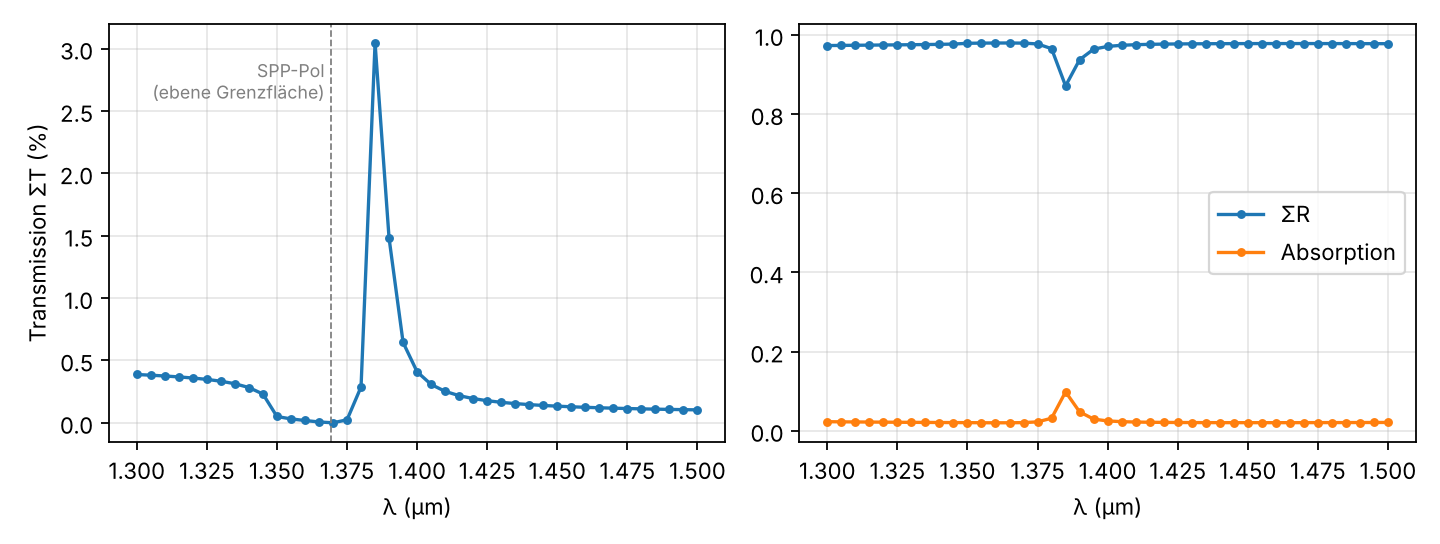
\includegraphics[width=\linewidth]{fig/v10_spec.png}
\caption{Silber-Lochgitter, $N_x=N_z=6$: Transmission (links), Reflexion und Absorption (rechts). Gestrichelt: Pol
des Oberflächenplasmons an der ebenen Silber-Luft-Grenzfläche.}
\end{figure}

\textbf{Worauf achten:} Die Brechzahl von Silber ist hier für alle Wellenlängen gleich, wie im Referenzfall des
Buchs. Für quantitative Spektren ein dispersives Modell oder eine Tabelle einsetzen
(Abschnitt~\ref{sec:conf-dispersion}), z.\,B.\ das Drude--Lorentz-Modell aus
\file{examples/dispersive\_metal\_grating.json}. Die Lage des Peaks verschiebt sich mit $N$; Spektren für $N=6,8,10$
vergleichen.

%-------------------------------------------------------------------------------------------
\section{Einzelner Steg mit PML}
\textbf{Aufgabe:} Ein Siliziumsteg (0,3\um{} breit, 0,2\um{} hoch) auf Glas. Wie viel Licht streut er?
\begin{lstlisting}[language=json]
{ "dimension": "1D", "solver": "rcwa", "truncation": { "Nx": 60 }, "period_um": { "x": 4.0 },
  "incidence": { "lambda_um": 0.6328, "phi_deg": 0, "delta_deg": 0 },
  "materials": { "air": {"n": 1.0}, "glass": {"n": 1.5}, "si": {"n": [3.88, 0.02]} },
  "superstrate": "air", "substrate": "glass",
  "layers": [ { "type": "lamellar1d", "thickness_um": 0.2,
                "breakpoints_um": [0, 1.85, 2.15, 4.0], "materials": ["air", "si", "air"] } ],
  "aperiodic": { "pml": { "x": { "width_um": 0.8, "beta": 1.0 } } } }
\end{lstlisting}
\textbf{Ergebnis} (8\,s): Streubreite nach oben 0,329\um, nach unten 0,370\um, absorbiert 0,023\um. Bei
$\varphi=20^\circ$ (automatisch Streufeldformulierung): 0,340 / 0,345 / 0,042\um.

\textbf{Worauf achten:} Zellbreite und $N$ gemeinsam erhöhen und prüfen, dass die Summe stabil ist. Die Struktur
muss vollständig im physikalischen Bereich $[0{,}8;\,3{,}2]$\um{} liegen.

%-------------------------------------------------------------------------------------------
\section{Säule unter einem Gauß-Strahl (Zylinder)}
\textbf{Aufgabe:} Eine SiN-Säule ($n=1{,}45$, Radius 0,4\um, Höhe 0,3\um) auf Glas, beleuchtet von einem fokussierten
Gauß-Strahl (Taille 0,5\um), 0,9--1,1\um.

\textbf{Konfiguration:} \file{examples/cyl\_pillar\_beam.json} (Abschnitt~\ref{sec:zylinder}).

\textbf{Ergebnis} (14\,s für drei Wellenlängen): Bei 0,9\um{} werden 4,74\,\% reflektiert und 95,24\,\% transmittiert,
je zur Hälfte in den Harmonischen $m=\pm1$ (x-Polarisation). \texttt{C\_A} liegt zwischen $-1{,}7\cdot10^{-4}$ und
$1{,}2\cdot10^{-4}$ -- bei verlustfreien Materialien ein Maß für die Genauigkeit des Spektrums; \key{kappa\_max}
erhöhen, wenn mehr nötig ist.

%-------------------------------------------------------------------------------------------
\section{Freiform-Profil mit Hinterschnitt als NURBS}
\index{NURBS}\index{Ueberhang@Überhang}\index{Schichttyp!profile1d@\texttt{profile1d}!nurbs@\texttt{nurbs}}%
\textbf{Aufgabe:} Eine Lackline mit überhängendem Kopf („Pilz“, Periode 0,3\um) auf Silizium, TM, 633\,nm unter
$10^\circ$. Wie viel wird reflektiert? Als Funktion $y=g(x)$ geht das nicht, eine STEP-Datei ist nicht nötig.
\begin{lstlisting}[language=json]
{ "dimension": "1D", "solver": "rk", "truncation": { "Nx": 15 }, "period_um": { "x": 0.3 },
  "incidence": { "lambda_um": 0.633, "phi_deg": 10, "psi_deg": 0, "delta_deg": 90 },
  "materials": { "air": {"n": 1.0}, "resist": {"n": 1.6}, "si": {"n": [3.88, 0.02]} },
  "superstrate": "air", "substrate": "si", "rk": { "tol": 1e-8 },
  "layers": [ { "type": "profile1d", "shape": "nurbs", "below": "resist", "above": "air",
    "nurbs": { "degree": 2, "knots": [0,0,0, 1,1, 2,2, 3,3, 4,4, 5,5, 6,6, 7,7,7],
      "points_um": [[0.0, 0.02], [0.065, 0.02], [0.13, 0.02], [0.14, 0.06], [0.12, 0.09],
                    [0.05, 0.10], [0.08, 0.13], [0.15, 0.19], [0.22, 0.13], [0.25, 0.10],
                    [0.18, 0.09], [0.16, 0.06], [0.17, 0.02], [0.235, 0.02], [0.3, 0.02]] } } ] }
\end{lstlisting}
Die Kurve besteht aus sieben quadratischen Bézierstücken (innere Knoten doppelt): Restschicht, Stiel links, Kopf
links (nach außen, der Überhang), Kopf oben, Kopf rechts, Stiel rechts, Restschicht. Sie beginnt bei $(0;\,0{,}02)$
und endet eine Periode weiter auf derselben Höhe.

\textbf{Ergebnis:} $R_0=0{,}25484$ (RK, 23\,s); RCWA mit 80 Scheiben liefert dasselbe auf $3\cdot10^{-6}$ in 3\,s.

\textbf{Worauf achten:} Die Linie läuft insgesamt von links nach rechts, \key{below} liegt darunter. Die Höhe der
Schicht ist ohne \key{depth\_um} die Oberkante der Kurve (hier 0,16\um). Ein Fehler wie
\texttt{/layers/0: [NURBS\_PERIOD]} heißt: der letzte Punkt liegt nicht genau eine Periode rechts vom ersten.
Selbstschnitte (auch mit dem Nachbarn der nächsten Periode) meldet \texttt{NURBS\_SELF\_INTERSECTION}.

%-------------------------------------------------------------------------------------------
\section{Littrow-Gitter optimieren}
\index{Littrow}%
\textbf{Aufgabe:} Ein Aluminium-Lamellengitter (Periode 0,5\um, TM) so auslegen, dass möglichst viel Licht in die
Ordnung $-1$ zurückgeht.

\textbf{Lösung:} \file{examples/python/optimize\_littrow.py} oder in der GUI \gui{Optimierung} $\to$
\gui{Littrow-Vorlage laden}. Parameter sind Tiefe (\val{/layers/0/thickness\_um}) und Stegbreite
(\val{/layers/0/breakpoints\_um/1}). Das Skript vergleicht das Ergebnis von L-BFGS-B mit einem Rasterscan; jede
Auswertung mit Gradient kostet nur etwa 1,3--2,5 Vorwärtsrechnungen, unabhängig von der Zahl der Parameter.

%-------------------------------------------------------------------------------------------
\section{Konvergenzstudie als Sweep}
\index{Konvergenz!Studie}%
\begin{lstlisting}[language=json]
"sweep": { "parameter": "/truncation/Nx", "values": [10, 20, 40, 80] }
\end{lstlisting}
Mit \file{plot\_efficiencies.py \ldots{} --x sweep\_value} entsteht direkt die Konvergenzkurve. In 2D müssen $N_x$ und
$N_z$ gemeinsam wachsen; dafür eine Python-Schleife verwenden.

\chapter{Fehlersuche}\label{ch:probleme}

\section{Fehlermeldungen}
\cmd{fgsolve} meldet Fehler als \texttt{fgsolve: error: <Quelldatei>:<Zeile>: <Meldung>} und endet mit Code 3; Python
wirft \texttt{fg.FourierGratingError}. Die häufigsten Meldungen:
\begin{center}
\small
\begin{longtable}{>{\raggedright\arraybackslash}p{6.2cm}>{\raggedright\arraybackslash}p{8.4cm}}
\toprule
Meldung & Ursache und Abhilfe \\
\midrule
\endhead
\texttt{cannot open configuration file \ldots} & Pfad falsch oder Datei nicht lesbar \\
\texttt{[json.exception.parse\_error\ldots]} & Kein gültiges JSON: Komma zu viel, Kommentar \texttt{//} in der Datei,
fehlende Anführungszeichen \\
\texttt{[json.exception.out\_of\_range.403] key 'x' not found} & Pflichtschlüssel fehlt oder ist falsch geschrieben
(z.\,B.\ \key{thickness\_um}) \\
\texttt{material 'x' needs 'n', 'eps', \ldots} & Materialangabe fehlt \\
\texttt{unknown material 'x'} & Name in einer Schicht nicht in \key{materials} \\
\texttt{superstrate must be isotropic and lossless} & Superstrat absorbiert oder ist anisotrop -- reelles $n$ verwenden;
Verluste gehören in Schichten oder das Substrat \\
\texttt{lamellar: breakpoints/materials} & Zahl der Stellen $\neq$ Zahl der Materialien $+1$ \\
\texttt{unknown profile shape 'x'} & \key{shape} nicht \val{sinus}, \val{triangle} oder \val{points} \\
\texttt{unknown factorization 'x'} & Schreibweise prüfen (Tabelle~\ref{tab:faktorisierung}) \\
\texttt{factorization not applicable \ldots} & Variante passt nicht zum Schichttyp $\to$ \val{auto} \\
\texttt{polygon2d: inclusion needs 'vertices\_um' or 'rectangle\_um'} & Einschluss ohne Geometrie \\
\texttt{sweep: parameter '\ldots' not found} & JSON-Pointer zeigt ins Leere; optionalen Block anlegen \\
\texttt{sweep: parameter '\ldots' is not a number} & Pointer zeigt auf eine Liste oder ein Objekt (z.\,B.\
\val{/materials/au/n} bei \val{[Re, Im]}; richtig: \val{/materials/au/n/0}) \\
\texttt{/materials/x/n/table: lambda \ldots{} um outside [\ldots] um} & Scanpunkt außerhalb der Tabelle: Tabelle
erweitern, Scan einschränken oder \val{"extrapolate": "constant"} \\
\texttt{\ldots/sellmeier: lambda \ldots{} at the pole \ldots} & Wellenlänge auf einem Pol $\sqrt{C_k}$ der
Sellmeier-Formel \\
\texttt{\ldots/sellmeier: lambda \ldots{} um outside [\ldots] um (range\_um)} & außerhalb des
Gültigkeitsbereichs der Formel \\
\texttt{\ldots: the superstrate must be lossless at every scan point} & dispersives Superstrat mit Verlusten an einem
Scanpunkt \\
\texttt{\ldots dispersive eps\_tensor entries} (Code 2) & Modell in \key{eps\_tensor}; \key{eps\_principal} mit
\key{euler\_deg} verwenden \\
\texttt{no material jumps found along the axis, give breakpoints\_um} & ASR mit \val{auto} ohne Lamellen/Polygone \\
\texttt{CUDA backend requested but not available} & \val{"backend": "cuda"} ohne GPU-Build oder Gerät $\to$ \val{auto} \\
\texttt{\ldots NotImplemented \ldots M\textit{x}} (Code 2) & Funktion spezifiziert, aber noch nicht umgesetzt; z.\,B.\
\val{cad} ohne Slicer \\
\bottomrule
\end{longtable}
\end{center}

\section{Verdächtige Ergebnisse}
\begin{center}
\small
\begin{longtable}{>{\raggedright\arraybackslash}p{5.2cm}>{\raggedright\arraybackslash}p{9.4cm}}
\toprule
Symptom & Ursache und Abhilfe \\
\midrule
\endhead
\texttt{sum R+T} $\neq1$ bei verlustfreien Materialien & $N$ zu klein, ungeeignete Faktorisierung, oder Geometriefehler
(z.\,B.\ letzte Lamellenstelle $\neq$ Periode) \\
$R+T>1$ bei Metallen & \val{FFF\_iso} gewählt $\to$ \val{auto}; oder $N$ erhöhen \\
negative Absorption & wie oben; bei \val{fp32} \key{precision} auf \val{fp64} \\
Ergebnis springt mit $N$ & Resonanz in der Nähe -- Spektrum statt Einzelwert vergleichen; bei Metall-TM ASR verwenden \\
Ergebnis hängt stark von \key{slices} ab & Profil mit RCWA: Scheibenzahl erhöhen oder RK verwenden \\
TE und TM vertauscht & \key{delta\_deg}: 0 = s (TE), 90 = p (TM) \\
Ordnung fehlt in der Tabelle & sie propagiert nicht (evaneszent) -- Gittergleichung prüfen \\
keine T-Ordnungen & Substrat absorbiert ($\operatorname{Im}n>0$); Transmission ist dann Absorption \\
Spiegelbild der Erwartung & Vorzeichen von $\varphi$ oder $\psi$; Ordnung $-1$ läuft bei $\varphi>0$ zurück zur Einfallsseite \\
Einschlüsse verschiedener Materialien berühren sich (\val{polygon2d}) & mit \val{FFF\_B} unzuverlässig (Normalenfeld dort
undefiniert, nicht geprüft) $\to$ Einschlüsse trennen oder \val{laurent} \\
Absorption bei \val{"n": [3.88, -0.02]} negativ & Vorzeichen: Verluste haben $\operatorname{Im}n>0$ \\
\bottomrule
\end{longtable}
\end{center}

\section{Rechenzeit und Speicher}
\begin{center}
\small
\begin{longtable}{>{\raggedright\arraybackslash}p{5.2cm}>{\raggedright\arraybackslash}p{9.4cm}}
\toprule
Symptom & Abhilfe \\
\midrule
\endhead
RK sehr langsam & 2D oder großes $N$ $\to$ RCWA mit Treppe; \key{rk.tol} lockern ($10^{-5}$) \\
2D-Rechnung dauert Stunden & $N$ zu groß (Zeit $\propto n^3$); GPU verwenden; mit kleinem $N$ beginnen \\
Speicher reicht nicht & \key{threads.scan} verringern (jeder parallele Scanpunkt braucht eigenen Speicher); $N$ senken \\
nur ein Kern ausgelastet & \texttt{FG\_NUM\_THREADS}/\texttt{OMP\_NUM\_THREADS} prüfen; viele Scheiben:
\val{"reduction": "tree"} \\
GPU wird nicht benutzt & Matrix kleiner als \key{backend\_threshold}; \cmd{fgsolve --info} prüfen; Python:
\texttt{fg.core\_variant()} \\
GPU-Ergebnis weicht ab & \val{fp32} aktiv (RTX 3090: Standard) -- \key{precision} \val{fp64} für Endergebnisse \\
\bottomrule
\end{longtable}
\end{center}

\section{GUI}
\begin{center}
\small
\begin{longtable}{>{\raggedright\arraybackslash}p{5.2cm}>{\raggedright\arraybackslash}p{9.4cm}}
\toprule
Symptom & Abhilfe \\
\midrule
\endhead
Rechnungen sind weg & Adresse ohne \texttt{?s=}-Kennung geöffnet $\to$ Lesezeichen mit Kennung verwenden \\
Rechnung steht als „Server wurde neu gestartet“ & neu einreichen \\
Rechnung wartet lange & Platz in der Warteschlange unter \gui{Rechnungen}; nur eine Rechnung läuft gleichzeitig \\
Fehler am falschen Reiter angezeigt & die GUI rät den Reiter aus dem Meldungstext; Meldung selbst lesen \\
Seite \gui{CAD} meldet fehlenden Slicer & Server ohne CAD-Slicer gebaut (Seite \gui{System}) \\
Seite bleibt leer (hinter nginx) & WebSocket-Header fehlen (Betreiber) \\
\bottomrule
\end{longtable}
\end{center}

\section{Fehler melden}
Ein guter Fehlerbericht enthält die Konfiguration (JSON), die Ausgabe von \cmd{fgsolve --info} bzw.\
\texttt{fg.\_\_version\_\_} und \texttt{fg.core\_variant()}, die vollständige Meldung und -- bei falschen Ergebnissen
-- die Erwartung mit Quelle. Issues im Repository \file{PhotonPower/FourierGrating}.

\appendix
\chapter{Kurzreferenz der Konfiguration}\label{anh:schluessel}
\small
\begin{longtable}{>{\raggedright\arraybackslash}p{5.0cm}>{\raggedright\arraybackslash}p{2.4cm}>{\raggedright\arraybackslash}p{7.0cm}}
\toprule
Schlüssel & Standard & Kurzbeschreibung \\
\midrule
\endhead
\multicolumn{3}{l}{\textbf{Grundeinstellungen}} \\
\key{dimension} & Pflicht & \val{1D} | \val{2D} \\
\key{solver} & \val{rcwa} & \val{rcwa} | \val{rk} \\
\key{truncation.Nx}, \key{.Nz} & 10, 0 & Fourierordnungen \\
\key{period\_um.x}, \key{.z} & Pflicht, 0 & Perioden \\
\multicolumn{3}{l}{\textbf{Einfall} (Zahl, Liste oder \{from, to, steps\})} \\
\key{incidence.lambda\_um} & Pflicht & Wellenlänge \\
\key{incidence.phi\_deg}, \key{psi\_deg}, \key{delta\_deg} & 0 & Winkel, Polarisation \\
\key{incidence.type} & -- & \val{gaussian\_beam}, \val{plane\_wave} (Zylinder) \\
\key{incidence.waist\_um}, \key{focus\_y\_um}, \key{polarization} & --, 0, \val{x} & Gauß-Strahl \\
\multicolumn{3}{l}{\textbf{Sweep}} \\
\key{sweep.parameter} & -- & JSON-Pointer auf eine Zahl \\
\key{sweep.values} & -- & Zahl, Liste oder Bereich \\
\multicolumn{3}{l}{\textbf{Materialien, Halbräume}} \\
\key{materials.<name>.n} \textbar{} \key{eps} \textbar{} \key{eps\_tensor} \textbar{} \key{eps\_principal} & -- & genau eine Angabe \\
\key{materials.<name>.euler\_deg} & [0,0,0] & zu \key{eps\_principal}, $z$-$x$-$z$ \\
Materialwert & -- & Zahl, \val{[Re, Im]} oder Modell: \key{sellmeier}, \key{cauchy}, \key{drude\_lorentz},
\key{table} (Abschnitt~\ref{sec:conf-dispersion}) \\
\key{table.file} | \key{table.data} & Pflicht & CSV-Datei oder Zeilen \\
\key{table.unit}, \key{interpolation}, \key{extrapolate} & \val{um}, \val{linear}, \val{error} & \val{nm}, \val{eV};
\val{cubic}; \val{constant} \\
\key{superstrate}, \key{substrate} & Pflicht & Materialnamen \\
\multicolumn{3}{l}{\textbf{Schichten} (\key{layers}, von unten nach oben)} \\
\val{homogeneous} & & \key{thickness\_um}, \key{material} \\
\val{lamellar1d} & & \key{thickness\_um}, \key{breakpoints\_um}, \key{materials} \\
\val{profile1d} & & \key{depth\_um}, \key{below}, \key{above}, \key{shape}, \key{x0\_um}, \key{apex\_x\_um},
\key{x\_um}, \key{y\_um}, \key{slices} \\
\val{polygon2d} & & \key{thickness\_um}, \key{background}, \key{inclusions} (\key{material}, \key{vertices\_um} |
\key{rectangle\_um}), \key{normal\_field} \\
\val{contour2d} & & \key{thickness\_um}, \key{background}, \key{regions} (\key{material}, \key{circle} | \key{ellipse} |
\key{polygon\_um} | \key{nurbs}, \key{holes}), \key{normal\_field} \\
\val{profile2d} & & \key{depth\_um}, \key{below}, \key{above}, \key{shape}, \key{x0\_um}, \key{z0\_um}, \key{slices},
\key{z\_samples} \\
\val{cad} & & \key{file} | \key{step}, \key{unit}, \key{axes}, \key{y\_range\_um}, \key{cell\_origin\_um},
\key{background}, \key{bodies}, \key{overlap}, \key{periodic\_union}, \key{slicing}, \key{normal\_field} \\
\val{rings} & & \key{thickness\_um}, \key{radii\_um}, \key{materials} \\
alle & \val{auto} & \key{factorization} \\
\multicolumn{3}{l}{\textbf{Löser und Leistung}} \\
\key{rk.tableau}, \key{rk.tol} & \val{gauss2}, $10^{-8}$ & Runge--Kutta \\
\key{rcwa.slices} & 40 & Scheiben je Profilschicht \\
\key{backend}, \key{backend\_threshold} & \val{auto}, 160 & CPU/GPU \\
\key{precision}, \key{precision\_fallback} & \val{auto}, auto & Genauigkeit \\
\key{threads.scan}, \key{.slices}, \key{.blas} & auto, auto, 1 & Threads \\
\key{reduction} & \val{sequential} & \val{tree}: parallele Verkettung \\
\key{split\_polarizations} & \val{false} & TE/TM getrennt (1D, $\psi=0$, isotrop) \\
\key{fft\_sampling} & \val{false} & FFT für abgetastete Koeffizienten \\
\key{growth\_limit} & 0 & Stabilitätsscheiben (0 = auto) \\
\key{checkpoint\_every} & 1 & Gradienten-Speicher \\
\multicolumn{3}{l}{\textbf{Erweiterungen}} \\
\key{coordinate\_transform.x}, \key{.z} & -- & ASR: \key{type}, \key{eta}, \key{breakpoints\_um} \\
\key{aperiodic} & -- & PML: \key{pml.x}, \key{.z} (\key{width\_um}, \key{beta}), \key{formulation}, \key{excitation} \\
\key{superstrate\_structure}, \key{substrate\_structure} & -- & strukturierte Halbräume \\
\key{scattered\_field} & \val{false} & Streufeld bei periodischen Gittern \\
\key{cylindrical} & -- & \key{symmetry}, \key{harmonics}, \key{spectrum}, \key{factorization} \\
\multicolumn{3}{l}{\textbf{Nahfeld und Ausgabe}} \\
\key{nearfield.enabled} & \val{false} & \\
\key{nearfield.horizontal\_y\_um}, \key{vertical\_z\_um} & 0, 0 & Lage der Schnitte \\
\key{nearfield.y\_range\_um} & $[-0{,}2;\,0{,}5]$ & \\
\key{nearfield.nx}, \key{ny}, \key{nz}, \key{periods} & 400, 300, 200, 1 & \\
\key{nearfield.reconstruction}, \key{field} & \val{fff}, \val{total} & \\
\key{output.dir}, \key{output.efficiencies} & \val{out}, \val{efficiencies.csv} & \\
\key{output.materials} & -- & \file{materials.csv}: $n$, $\varepsilon$ je Wellenlänge \\
\bottomrule
\end{longtable}
\normalsize

\chapter{Befehlsreferenz}\label{anh:cli}
Dieser Anhang führt alle Programme, Skripte, Python-Funktionen, Umgebungsvariablen und Build-Optionen vollständig
auf. Er ist aus dem Quellcode erstellt; der Test \file{tests/python/test\_handbook\_reference.py} prüft, dass jeder
öffentliche Python-Name, jede Option von \cmd{fgsolve} und \cmd{fgbench}, jede Umgebungsvariable des Kerns und jede
CMake-Option hier vorkommt. Die Konfigurationsschlüssel stehen in Anhang~\ref{anh:schluessel}.

% ============================================================================================
\section{\texttt{fgsolve}}\label{sec:ref-fgsolve}
\index{fgsolve@\texttt{fgsolve}}
\begin{lstlisting}[style=shell]
fgsolve <config.json>
fgsolve --profile <config.json>
fgsolve --cad-report <config.json>
fgsolve --info | --version | --help
\end{lstlisting}
Ausgewertet wird nur das erste Argument; Optionen lassen sich nicht kombinieren (außer \texttt{-{}-profile} mit
der Datei).
\begin{center}
\small
\begin{tabularx}{\linewidth}{>{\raggedright\arraybackslash}p{4.4cm}Y}
\toprule
Aufruf & Wirkung \\
\midrule
\texttt{fgsolve <config.json>}\index{fgsolve@\texttt{fgsolve}!Rechnung} & Rechnet alle Sweep-Werte und Scanpunkte
(Scanpunkte parallel), gibt je Scanpunkt einen Block auf dem Terminal aus (Abschnitt~\ref{ch:ausgabe}) und schreibt
\file{<output.dir>/<output.efficiencies>}, mit \key{output.materials} zusätzlich \file{materials.csv}. Mit
\val{"nearfield": \{"enabled": true\}} folgen \file{nearfield\_horizontal/} und \file{nearfield\_vertical/} für den
ersten Scanpunkt des ersten Sweep-Werts. \key{output.dir} gilt relativ zum Arbeitsverzeichnis. \\
\texttt{-{}-profile <config.json>}\index{--profile@\texttt{-{}-profile}} & wie oben, dazu die Rechenzeit je Abschnitt
(über alle Threads summiert) auf dem Terminal und in \file{<output.dir>/profile.json} \\
\texttt{-{}-cad-report <config.json>}\index{--cad-report@\texttt{-{}-cad-report}} & Geometrieprüfung und Bandzerlegung
der \val{cad}-Schichten als JSON auf der Standardausgabe; STEP-Pfade relativ zur Konfiguration
(Abschnitt~\ref{ch:cad}). Rechnet nicht. \\
\texttt{-{}-info}\index{--info@\texttt{-{}-info}} & Version, CPU-Backend, CUDA-Backend (nicht gebaut, gebaut ohne Gerät
oder Name der GPU) und CAD-Slicer (Nurbforge oder nicht gebaut) \\
\texttt{-{}-version}\index{--version@\texttt{-{}-version}} & \texttt{FourierGrating 0.18.0} \\
\texttt{-{}-help}\index{--help@\texttt{-{}-help}} & Kurzhilfe \\
\bottomrule
\end{tabularx}
\end{center}
\paragraph{Rückgabecodes.}\index{Rückgabecode}
\begin{center}
\small
\begin{tabularx}{\linewidth}{cY}
\toprule
Code & Bedeutung \\
\midrule
0 & Erfolg; bei \texttt{-{}-cad-report}: keine Fehler gefunden \\
1 & ohne Argument aufgerufen (Kurzhilfe) \\
2 & Funktion spezifiziert, aber nicht umgesetzt; Meldung \texttt{fgsolve: <Text>} auf der Fehlerausgabe \\
3 & Fehler in Konfiguration oder Rechnung; Meldung \texttt{fgsolve: error: <Text>} \\
4 & \texttt{-{}-cad-report}: der Bericht enthält Fehler \\
\bottomrule
\end{tabularx}
\end{center}

% ============================================================================================
\section{\texttt{fgbench}}\label{sec:ref-fgbench}
\index{fgbench@\texttt{fgbench}}
\begin{lstlisting}[style=shell]
fgbench [--sizes 256,512,1024] [--orders 4,6,8] [--repeat 1]
\end{lstlisting}
\begin{center}
\small
\begin{tabularx}{\linewidth}{llY}
\toprule
Option & Standard & Wirkung \\
\midrule
\texttt{-{}-sizes}\index{--sizes@\texttt{-{}-sizes}} & \val{256,512,1024} & Matrixgrößen $n$ für ZGEMM, LU-Lösung mit $n$
rechten Seiten und allgemeines Eigenproblem (komplexe Zufallsmatrizen) \\
\texttt{-{}-orders}\index{--orders@\texttt{-{}-orders}} & \val{4,6,8} & Trunkierungen $N=N_x=N_z$ für eine RCWA-Rechnung
des Silber-Lochgitters V10 bei $\lambda=1{,}388$\um \\
\texttt{-{}-repeat}\index{--repeat@\texttt{-{}-repeat}} & \val{1} & Wiederholungen; gemeldet wird die kürzeste Zeit \\
\bottomrule
\end{tabularx}
\end{center}
Die Ausgabe sind Markdown-Tabellen je Backend (\val{cpu}, mit GPU zusätzlich \val{cuda}). Optionen stehen paarweise
mit ihrem Wert; unbekannte Optionen werden ohne Meldung übergangen. Messwerte stehen in \file{docs/benchmarks.md}.

% ============================================================================================
\section{Skripte}\label{sec:ref-skripte}
\subsection*{\texttt{scripts/plot\_efficiencies.py}}\index{plot_efficiencies.py@\texttt{plot\_efficiencies.py}}
\begin{lstlisting}[style=shell]
plot_efficiencies.py <efficiencies.csv> [--x SPALTE] [--orders SEITE:n[:m] ...]
                     [--quantity efficiency|eff_s|eff_p]
                     [--lambda W] [--phi W] [--psi W] [--delta W] [--out DATEI]
\end{lstlisting}
\begin{center}
\small
\begin{tabularx}{\linewidth}{lY}
\toprule
Argument & Wirkung \\
\midrule
\texttt{csv} & \file{efficiencies.csv} von \cmd{fgsolve} \\
\texttt{-{}-x} & $x$-Achse: \val{sweep\_value}, \val{lambda\_um}, \val{phi\_deg}, \val{psi\_deg}, \val{delta\_deg};
Standard: die erste dieser Spalten, die sich ändert \\
\texttt{-{}-orders} & Ordnungen als \val{R:0}, \val{T:-1} oder \val{T:1:0} (2D); Standard: alle \\
\texttt{-{}-quantity} & \val{efficiency} (Standard), \val{eff\_s} oder \val{eff\_p} \\
\texttt{-{}-lambda}, \texttt{-{}-phi}, \texttt{-{}-psi}, \texttt{-{}-delta} & nur Zeilen mit diesem Wert der übrigen
Scanspalten \\
\texttt{-{}-out} & Abbildung in eine Datei schreiben statt anzeigen \\
\bottomrule
\end{tabularx}
\end{center}

\subsection*{\texttt{scripts/plot\_nearfield.py}}\index{plot_nearfield.py@\texttt{plot\_nearfield.py}}
\begin{lstlisting}[style=shell]
plot_nearfield.py <schnittverzeichnis> [--quantity absE2] [--part abs|re|im|phase] [--out DATEI]
plot_nearfield.py --demo <verzeichnis>
\end{lstlisting}
\begin{center}
\small
\begin{tabularx}{\linewidth}{lY}
\toprule
Argument & Wirkung \\
\midrule
\texttt{cut\_dir} & Verzeichnis eines Schnitts, z.\,B.\ \file{out/x/nearfield\_vertical} \\
\texttt{-{}-quantity} & Name einer \file{.npy}-Datei: \val{Ex} \ldots{} \val{Hz}, \val{absE2} (Standard), \val{absH2},
\val{Sy} \\
\texttt{-{}-part} & \val{abs} (Standard), \val{re}, \val{im}, \val{phase} \\
\texttt{-{}-out} & Abbildung in eine Datei schreiben \\
\texttt{-{}-demo DIR} & schreibt synthetische Testdaten nach \texttt{DIR} und zeichnet sie \\
\bottomrule
\end{tabularx}
\end{center}

\subsection*{Weitere Skripte}
\begin{center}
\small
\begin{tabularx}{\linewidth}{>{\raggedright\arraybackslash}p{5.6cm}Y}
\toprule
Aufruf & Wirkung \\
\midrule
\texttt{scripts/build\_docs.sh}\index{build_docs.sh@\texttt{build\_docs.sh}} & erzeugt
\file{docs/implementation\_plan/main.pdf} und \file{docs/handbuch/handbuch.pdf} (mit Stichwortverzeichnis) \\
\texttt{scripts/setup\_almalinux10.sh [-{}-with-cuda]}\index{setup_almalinux10.sh@\texttt{setup\_almalinux10.sh}} &
installiert Compiler, Bibliotheken, Python und \LaTeX{} unter AlmaLinux~10 (als root); \texttt{-{}-with-cuda}
zusätzlich das CUDA-Toolkit; \texttt{-h} Hilfe \\
\texttt{scripts\textbackslash setup\_windows.ps1 [-SkipMsys2Install]}\index{setup_windows.ps1@\texttt{setup\_windows.ps1}}
& installiert MSYS2 (falls nötig) und die UCRT64-Werkzeuge; nur CPU \\
\texttt{scripts\textbackslash msvc.cmd <befehl>}\index{msvc.cmd@\texttt{msvc.cmd}} & führt einen Befehl in der
Umgebung von MSVC 2022 x64 aus, z.\,B.\ \texttt{scripts\textbackslash msvc.cmd cmake -{}-preset win-msvc} \\
\texttt{python scripts/make\_cad\_examples.py}\index{make_cad_examples.py@\texttt{make\_cad\_examples.py}} & schreibt
die STEP-Dateien \file{examples/cad/*.step} und \file{tests/data/cad/*.step} (braucht \texttt{nurbforge>=0.6.0}) \\
\texttt{python3 scripts/proto\_cylindrical.py [fiber|offaxis]}\index{proto_cylindrical.py@\texttt{proto\_cylindrical.py}}
& Prototyp zu den Zylinderkoordinaten (Fasermoden, exzentrischer Kern); kein Teil des Lösers \\
\bottomrule
\end{tabularx}
\end{center}

% ============================================================================================
\section{Python-API}\label{sec:ref-python}
\index{Python-API}
Pakete: \texttt{fouriergrating} (CPU) und \texttt{fouriergrating-cuda12} (zusätzlich, mit CUDA-Kern); importiert wird
immer \texttt{import fouriergrating as fg}. Zusätze für \texttt{pip install fouriergrating[...]}: \val{pandas}
(\texttt{ScanResult.to\_pandas}), \val{materials} (PyYAML für den Import aus refractiveindex.info), \val{test}
(pytest, pandas, PyYAML).

Eine \emph{Konfiguration} \texttt{cfg} ist ein \texttt{dict} im JSON-Schema von Kapitel~\ref{ch:konfiguration} oder
der Pfad einer JSON-Datei (dann wie mit \texttt{load\_config} gelesen). Längen in \textmu m, Winkel in Grad.

\subsection{Funktionen des Moduls \texttt{fouriergrating}}
\begin{center}
\small
\begin{longtable}{>{\raggedright\arraybackslash}p{6.2cm}>{\raggedright\arraybackslash}p{8.4cm}}
\toprule
Aufruf $\to$ Rückgabe & Wirkung \\
\midrule
\endhead
\texttt{load\_config(path)} $\to$ \texttt{dict}\index{load_config@\texttt{load\_config}} & liest eine JSON-Datei;
\key{output.dir}, \key{file} von \val{cad}-Schichten und Tabellendateien gelten danach absolut \\
\texttt{solve(cfg, profile=False)} $\to$ \texttt{Result}\index{solve@\texttt{solve}} & erster Scanpunkt;
\key{sweep} wird übergangen. \texttt{profile=True}: Zeiten je Abschnitt in
\texttt{diagnostics["timings"]["scopes"]} \\
\texttt{solve\_scan(cfg, profile=False)} $\to$ \texttt{ScanResult}\index{solve_scan@\texttt{solve\_scan}} & alle
Sweep-Werte und Scanpunkte wie \cmd{fgsolve} (parallel) \\
\texttt{near\_field(cfg)} $\to$ \texttt{dict}\index{near_field@\texttt{near\_field}} & Nahfeldschnitte des ersten
Scanpunkts: \texttt{\{"horizontal", "vertical"\}}, je mit Achsen, \texttt{Ex} \ldots{} \texttt{Hz} (komplex),
\texttt{absE2}, \texttt{absH2}, \texttt{Sy}, \texttt{material} und \texttt{meta} \\
\texttt{material\_eps(cfg, name, lambda\_um)} $\to$ \texttt{complex} | \texttt{ndarray}%
\index{material_eps@\texttt{material\_eps}} & $\varepsilon$ des Materials \texttt{name}; eine Zahl ergibt
\texttt{complex}, ein Array ein Array derselben Form; \key{eps\_principal}: letzte Achse der Länge 3 \\
\texttt{set\_backend(preference="auto", threshold=160)}\index{set_backend@\texttt{set\_backend}} & Standard für
Konfigurationen ohne \key{backend}: \val{auto}, \val{cpu} oder \val{cuda} (sonst \texttt{ValueError}) \\
\texttt{get\_backend()} $\to$ \texttt{dict}\index{get_backend@\texttt{get\_backend}} &
\texttt{\{"backend", "backend\_threshold"\}} \\
\texttt{cuda\_available()} $\to$ \texttt{bool}\index{cuda_available@\texttt{cuda\_available}} & Kern mit
CUDA-Backend geladen und GPU nutzbar \\
\texttt{core\_variant()} $\to$ \texttt{str}\index{core_variant@\texttt{core\_variant}} & \val{"cpu"} oder
\val{"cuda12"} \\
\bottomrule
\end{longtable}
\end{center}

\subsection{Konstanten und Ausnahmen}
\begin{center}
\small
\begin{tabularx}{\linewidth}{>{\raggedright\arraybackslash}p{4.2cm}Y}
\toprule
Name & Bedeutung \\
\midrule
\texttt{\_\_version\_\_}\index{__version__@\texttt{\_\_version\_\_}} & Version des Kerns, z.\,B.\ \val{"0.18.0"} \\
\texttt{ORDER\_DTYPE}\index{ORDER_DTYPE@\texttt{ORDER\_DTYPE}} & NumPy-dtype der Ordnungen:
\texttt{n}, \texttt{m} (int32), \texttt{eff}, \texttt{eff\_s}, \texttt{eff\_p} (float64), \texttt{amp\_s},
\texttt{amp\_p} (complex128) \\
\texttt{FourierGratingError}\index{FourierGratingError@\texttt{FourierGratingError}} & Konfigurations- und
Rechenfehler; Unterklasse von \texttt{RuntimeError} \\
\texttt{NotImplementedError} & spezifiziert, aber nicht umgesetzt \\
\bottomrule
\end{tabularx}
\end{center}

\subsection{Klasse \texttt{Result}}\index{Result@\texttt{Result}}
Ergebnis eines Scanpunkts (Datenklasse).
\begin{center}
\small
\begin{tabularx}{\linewidth}{>{\raggedright\arraybackslash}p{4.2cm}Y}
\toprule
Feld / Methode & Inhalt \\
\midrule
\texttt{reflected}, \texttt{transmitted} & Ordnungen als Array mit \texttt{ORDER\_DTYPE}, nur ausbreitungsfähige \\
\texttt{absorption} & absorbierter Anteil der einfallenden Leistung \\
\texttt{diagnostics} & \texttt{dict}, Abschnitt~\ref{sec:diagnose} \\
\texttt{incidence} & \texttt{\{"lambda\_um", "phi\_deg", "psi\_deg", "delta\_deg"\}} \\
\texttt{scattering} & isolierte Strukturen: \texttt{\{"up", "down", "lateral", "absorbed"\}} in \textmu m (2D:
\textmu m$^2$), sonst \texttt{None} \\
\texttt{modal} & Modenanregung: \texttt{\{"incident", "reflected", "transmitted", "radiated"\}}, sonst \texttt{None} \\
\texttt{cylindrical} & Zylinder: \texttt{\{"reflected", "transmitted", "absorbed", "harmonics", \ldots\}}, sonst
\texttt{None} \\
\texttt{efficiency(side, n, m=0)} $\to$ \texttt{float}\index{efficiency@\texttt{efficiency}} & Effizienz der Ordnung
$(n,m)$ auf \val{"R"} oder \val{"T"}; 0, wenn sie nicht ausbreitungsfähig ist \\
\bottomrule
\end{tabularx}
\end{center}

\subsection{Klasse \texttt{ScanResult}}\index{ScanResult@\texttt{ScanResult}}
\begin{center}
\small
\begin{tabularx}{\linewidth}{>{\raggedright\arraybackslash}p{4.2cm}Y}
\toprule
Feld / Methode & Inhalt \\
\midrule
\texttt{points} & Liste der \texttt{Result}, alle Sweep-Werte nacheinander \\
\texttt{sweep\_parameter} & JSON-Pointer des Sweeps oder \val{""} \\
\texttt{columns} & \texttt{dict} von Arrays wie \file{efficiencies.csv}: \texttt{sweep\_value}, \texttt{lambda\_um},
\texttt{phi\_deg}, \texttt{psi\_deg}, \texttt{delta\_deg}, \texttt{side}, \texttt{n}, \texttt{m},
\texttt{efficiency}, \texttt{eff\_s}, \texttt{eff\_p}, \texttt{amp\_s}, \texttt{amp\_p} \\
\texttt{to\_pandas()}\index{to_pandas@\texttt{to\_pandas}} & \texttt{columns} als \texttt{pandas.DataFrame} \\
\bottomrule
\end{tabularx}
\end{center}

\subsection{Klasse \texttt{Simulation}}\index{Simulation@\texttt{Simulation}}
\texttt{Simulation(cfg)} baut die Schichtmodelle einmal. Ein Objekt ist nicht threadsicher; während einer Rechnung
ist der GIL freigegeben. Fehlende Einfallswerte kommen vom ersten Scanpunkt der Konfiguration.
\begin{center}
\small
\begin{longtable}{>{\raggedright\arraybackslash}p{6.4cm}>{\raggedright\arraybackslash}p{8.2cm}}
\toprule
Methode / Eigenschaft & Wirkung \\
\midrule
\endhead
\texttt{solve(lambda\_um=None, phi\_deg=None, psi\_deg=None, delta\_deg=None)} $\to$ \texttt{Result} & Rechnung mit
den vorhandenen Schichtmodellen \\
\texttt{smatrix(lambda\_um=None, phi\_deg=None, psi\_deg=None)} $\to$ \texttt{OrderSMatrix}%
\index{smatrix@\texttt{smatrix}} & S-Matrix in der s/p-Basis (Abschnitt~\ref{sec:smatrix}) \\
\texttt{set\_parameter(pointer, value)}\index{set_parameter@\texttt{set\_parameter}} & setzt eine Zahl der
Konfiguration; baut nur abhängige Schichten neu \\
\texttt{value\_and\_grad(objective, params, lambda\_um=None, phi\_deg=None, psi\_deg=None, delta\_deg=None)}
$\to$ \texttt{(float, ndarray)}\index{value_and_grad@\texttt{value\_and\_grad}} & Zielfunktion und Gradient nach den
Pointern \texttt{params} (diskrete Adjungierte, Kapitel~\ref{ch:optimierung}); setzt \texttt{last\_result} \\
\texttt{vjp(cotangents, params)} $\to$ \texttt{ndarray}\index{vjp@\texttt{vjp}} & Vektor-Jacobi-Produkt;
\texttt{cotangents} in der Form einer Zielfunktion \\
\texttt{last\_result}\index{last_result@\texttt{last\_result}} & \texttt{Result} der letzten
\texttt{value\_and\_grad}-Rechnung \\
\texttt{config}\index{config@\texttt{config}} & aktuelle Konfiguration als \texttt{dict} (Eigenschaft) \\
\texttt{model\_builds}\index{model_builds@\texttt{model\_builds}} & Zahl der bisher gebauten Schichtmodelle
(Eigenschaft) \\
\bottomrule
\end{longtable}
\end{center}
\paragraph{Zielfunktion.}\index{Zielfunktion} \texttt{objective} ist ein Mapping \texttt{\{("R", -1, 0): 1.0, ...\}}
oder eine Folge von \texttt{(side, n, m, weight)}; $L=\sum w\,e$. Isolierte Strukturen:
\texttt{\{("scattering", "up"): w, ("scattering", "down"): w, ("mode", "R", j): w, ("mode", "T", j): w\}}.

\subsection{Klasse \texttt{OrderSMatrix}}\index{OrderSMatrix@\texttt{OrderSMatrix}}
\begin{center}
\small
\begin{tabularx}{\linewidth}{>{\raggedright\arraybackslash}p{4.4cm}Y}
\toprule
Feld / Methode & Inhalt \\
\midrule
\texttt{orders} & Array $(n_f, 2)$ der Ordnungen $(n, m)$ \\
\texttt{alpha}, \texttt{gamma}, \texttt{beta\_sup}, \texttt{beta\_sub} & normierte Wellenzahlen je Ordnung (mal
\texttt{k0} ergibt 1/\textmu m); $\operatorname{Im}\beta>0$: evaneszent \\
\texttt{R\_top}, \texttt{T\_down}, \texttt{T\_up}, \texttt{R\_bottom} & Blöcke $2n_f\times2n_f$; Index $r$ ist die
s-, $n_f+r$ die p-Komponente der Ordnung $r$ \\
\texttt{k0} & $2\pi/\lambda$ in 1/\textmu m \\
\texttt{incidence} & Einfallsrichtung der Rechnung \\
\texttt{index(n, m=0)} $\to$ \texttt{int} & Index $r$ der Ordnung; \texttt{KeyError}, wenn sie nicht in der
Trunkierung liegt \\
\bottomrule
\end{tabularx}
\end{center}

\subsection{Modul \texttt{fouriergrating.cad}}\index{fouriergrating.cad@\texttt{fouriergrating.cad}}
\texttt{step} ist STEP-Text, der Pfad einer STEP-Datei oder \texttt{None} (dann die Datei der \val{cad}-Schicht).
\begin{center}
\small
\begin{tabularx}{\linewidth}{>{\raggedright\arraybackslash}p{5.6cm}Y}
\toprule
Aufruf $\to$ Rückgabe & Wirkung \\
\midrule
\texttt{cad.available()} $\to$ \texttt{bool}\index{available@\texttt{available}} & Kern mit CAD-Slicer gebaut \\
\texttt{cad.check(step, cfg)} $\to$ \texttt{dict}\index{check@\texttt{check}} & Geometrieprüfung und
Bandzerlegung: \texttt{ok}, \texttt{errors}, \texttt{warnings} (\texttt{code}, \texttt{message},
\texttt{where\_um}), \texttt{bands} \\
\texttt{cad.preview(step, cfg, y\_um)} $\to$ \texttt{str}\index{preview@\texttt{preview}} & SVG des Schnitts in der
Höhe \texttt{y\_um} (eine Zelle, Materialien farbig) \\
\texttt{cad.llm\_tool\_spec()} $\to$ \texttt{dict}\index{llm_tool_spec@\texttt{llm\_tool\_spec}} & Beschreibung von
\texttt{check} als Werkzeug für ein Sprachmodell (Name, Beschreibung, JSON-Schema) \\
\bottomrule
\end{tabularx}
\end{center}

\subsection{Modul \texttt{fouriergrating.materials}}\index{fouriergrating.materials@\texttt{fouriergrating.materials}}
\texttt{materials.from\_refractiveindex(path\_or\_text)} $\to$ \texttt{dict}%
\index{from_refractiveindex@\texttt{from\_refractiveindex}}: Materialobjekt aus einer YAML-Datei (Pfad oder Text)
der Datenbank refractiveindex.info (Abschnitt~\ref{sec:py-dispersion}); braucht PyYAML.

\subsection{Module \texttt{fouriergrating.torch} und \texttt{fouriergrating.jax}}
\begin{center}
\small
\begin{tabularx}{\linewidth}{>{\raggedright\arraybackslash}p{6.4cm}Y}
\toprule
Aufruf $\to$ Rückgabe & Wirkung \\
\midrule
\texttt{torch.efficiencies(sim, params, values, orders)} $\to$ \texttt{torch.Tensor}%
\index{efficiencies@\texttt{efficiencies}} & Effizienzen der \texttt{orders} (\texttt{(side, n, m)}) für die Werte
\texttt{values} (1D-Tensor, ein Eintrag je Pointer), differenzierbar \\
\texttt{jax.efficiency\_function(sim, params, orders)} $\to$ Funktion%
\index{efficiency_function@\texttt{efficiency\_function}} & \texttt{f(values)} mit eigener VJP; float64 einschalten
(\texttt{jax\_enable\_x64}) \\
\bottomrule
\end{tabularx}
\end{center}

% ============================================================================================
\section{Umgebungsvariablen}\label{sec:ref-env}
\begin{center}
\small
\begin{tabularx}{\linewidth}{lY}
\toprule
Variable & Wirkung \\
\midrule
\texttt{FG\_NUM\_THREADS}\index{FG_NUM_THREADS@\texttt{FG\_NUM\_THREADS}} & Gesamtzahl der Threads (sonst
\texttt{OMP\_NUM\_THREADS}, sonst alle Kerne) \\
\texttt{FG\_BACKEND}\index{FG_BACKEND@\texttt{FG\_BACKEND}} & \val{cpu}, \val{cuda}, \val{auto}; überschreibt
\key{backend} \\
\texttt{FG\_BACKEND\_THRESHOLD}\index{FG_BACKEND_THRESHOLD@\texttt{FG\_BACKEND\_THRESHOLD}} & überschreibt
\key{backend\_threshold} \\
\texttt{FG\_PRECISION}\index{FG_PRECISION@\texttt{FG\_PRECISION}} & überschreibt \key{precision} \\
\texttt{FG\_GPU\_STREAMS}\index{FG_GPU_STREAMS@\texttt{FG\_GPU\_STREAMS}} & Scheiben gleichzeitig auf der GPU
(Standard 4) \\
\texttt{FG\_CORE}\index{FG_CORE@\texttt{FG\_CORE}} & Python: \val{cpu} erzwingt den CPU-Kern, \val{cuda12} den
CUDA-Kern auch ohne nutzbare GPU; Standard: CUDA-Kern, wenn installiert und eine GPU nutzbar ist \\
\texttt{CUDA\_PATH}\index{CUDA_PATH@\texttt{CUDA\_PATH}} & Windows: Ort der CUDA-Bibliotheken \\
\texttt{NVIDIA\_TF32\_OVERRIDE}\index{NVIDIA_TF32_OVERRIDE@\texttt{NVIDIA\_TF32\_OVERRIDE}} & \val{0} schließt TF32
aus \\
\texttt{FG\_FGSOLVE}\index{FG_FGSOLVE@\texttt{FG\_FGSOLVE}} & Python-Tests: Pfad zu \cmd{fgsolve} für Vergleiche \\
\texttt{FG\_REGRESSION\_EXACT}\index{FG_REGRESSION_EXACT@\texttt{FG\_REGRESSION\_EXACT}} & Regressionstests:
\val{1} verlangt Bitgleichheit mit den Golden Files (gleiche Maschine und gleicher Compiler) \\
\texttt{FG\_REGRESSION\_UPDATE}\index{FG_REGRESSION_UPDATE@\texttt{FG\_REGRESSION\_UPDATE}} & Regressionstests:
\val{1} schreibt die Golden Files neu (nur mit Begründung im \file{CHANGELOG.md}) \\
\texttt{FG\_GUI\_*} & GUI, siehe Abschnitt~\ref{sec:gui-betrieb} \\
\bottomrule
\end{tabularx}
\end{center}

% ============================================================================================
\section{Build: CMake-Optionen, Presets und Tests}\label{sec:ref-cmake}
\index{CMake}
\begin{center}
\small
\begin{tabularx}{\linewidth}{>{\raggedright\arraybackslash}p{5.0cm}lY}
\toprule
Option & Standard & Wirkung \\
\midrule
\texttt{FG\_ENABLE\_CUDA}\index{FG_ENABLE_CUDA@\texttt{FG\_ENABLE\_CUDA}} & \val{OFF} & CUDA-Backend bauen \\
\texttt{FG\_ENABLE\_OPENMP}\index{FG_ENABLE_OPENMP@\texttt{FG\_ENABLE\_OPENMP}} & \val{ON} & OpenMP für Scans und
Scheiben \\
\texttt{FG\_ENABLE\_HDF5}\index{FG_ENABLE_HDF5@\texttt{FG\_ENABLE\_HDF5}} & \val{OFF} & bindet HDF5 ein; die
Nahfeldausgabe ist derzeit \file{.npy} \\
\texttt{FG\_ENABLE\_NURBFORGE}\index{FG_ENABLE_NURBFORGE@\texttt{FG\_ENABLE\_NURBFORGE}} & \val{OFF} & CAD-Slicer
(Schichttyp \val{cad}); lädt Nurbforge per FetchContent \\
\texttt{FG\_NURBFORGE\_TAG}\index{FG_NURBFORGE_TAG@\texttt{FG\_NURBFORGE\_TAG}} & \val{v0.6.0} & Version von
Nurbforge \\
\texttt{FG\_BUILD\_TESTS}\index{FG_BUILD_TESTS@\texttt{FG\_BUILD\_TESTS}} & \val{ON} & Unit-, Validierungs- und
Regressionstests \\
\texttt{FG\_BUILD\_APPS}\index{FG_BUILD_APPS@\texttt{FG\_BUILD\_APPS}} & \val{ON} & \cmd{fgsolve} und \cmd{fgbench} \\
\texttt{FG\_BUILD\_PYTHON}\index{FG_BUILD_PYTHON@\texttt{FG\_BUILD\_PYTHON}} & \val{OFF} & Python-Modul
(\texttt{pip install} über scikit-build setzt \val{ON}) \\
\texttt{FG\_PYTHON\_PACKAGE}\index{FG_PYTHON_PACKAGE@\texttt{FG\_PYTHON\_PACKAGE}} & \val{fouriergrating} & Paket, in
das \texttt{\_core} kommt (\val{fouriergrating} oder \val{fouriergrating\_cuda12}) \\
\texttt{FG\_WARNINGS\_AS\_ERRORS}\index{FG_WARNINGS_AS_ERRORS@\texttt{FG\_WARNINGS\_AS\_ERRORS}} & \val{OFF} &
Warnungen als Fehler (CI) \\
\bottomrule
\end{tabularx}
\end{center}

\paragraph{Presets.}\index{Preset} Jedes Preset gibt es für \texttt{cmake -{}-preset}, \texttt{cmake -{}-build -{}-preset}
und \texttt{ctest -{}-preset}; gebaut wird nach \file{build/<preset>}.
\begin{center}
\small
\begin{tabularx}{\linewidth}{lY}
\toprule
Preset & Zweck \\
\midrule
\val{cpu-release} & Linux/macOS, Release, nur CPU (Standard) \\
\val{cpu-debug} & Debug mit AddressSanitizer und UBSan \\
\val{cpu-tsan} & ThreadSanitizer, ohne OpenMP \\
\val{cpu-cad} & wie \val{cpu-release}, mit CAD-Slicer \\
\val{cuda-release} & mit CUDA-Backend (Architekturen 86, 89) \\
\val{win-release}, \val{win-cad} & Windows mit MSYS2/UCRT64-GCC, ohne bzw.\ mit CAD-Slicer \\
\val{win-cuda} & Windows mit MSYS2-GCC und CUDA (Architektur 86) \\
\val{win-msvc}, \val{win-msvc-cuda} & Windows mit MSVC (über \texttt{scripts\textbackslash msvc.cmd}), ohne bzw.\ mit
CUDA \\
\bottomrule
\end{tabularx}
\end{center}

\paragraph{Tests.}\index{ctest@\texttt{ctest}}
\begin{lstlisting}[style=shell]
ctest --preset cpu-release                 # alle Tests
ctest --preset cpu-release -L unit         # nur eine Gruppe: unit | validation | regression
ctest --preset cpu-release -R V23c         # Tests, deren Name den regulären Ausdruck enthält
pytest tests/python                        # Python-Tests (pip install .[test])
\end{lstlisting}


\chapter{Beispieldateien und Referenzfälle}\label{anh:beispiele}
\section{Beispiele in \file{examples/}}
\begin{center}
\small
\begin{tabularx}{\linewidth}{lY}
\toprule
Datei & Fall \\
\midrule
\file{v1\_fresnel\_interface.json} & ebene Grenzfläche, konischer Einfall (Fresnel) \\
\file{v3\_lamellar\_dielectric.json} & dielektrisches Lamellengitter, RCWA \\
\file{v3\_lamellar\_rk\_scan.json} & dasselbe mit RK und Scan \\
\file{v4\_al\_sinus\_te.json}, \file{v4\_al\_sinus\_tm.json} & Aluminium-Sinusgitter \\
\file{v5\_glass\_deep\_te.json} & tiefes Glasgitter in Transmission \\
\file{echelette\_au\_scan.json} & Gold-Echelette, RK, Winkel-Scan \\
\file{v7\_cobalt\_anisotropic.json} & anisotropes Kobaltgitter \\
\file{v10\_hole\_array.json} & Silber-Lochgitter (2D) \\
\file{v15\_circular\_pillars.json} & Kreissäulen mit \val{contour2d} \\
\file{nearfield\_lamellar\_1d.json} & Nahfeld 1D \\
\file{nearfield\_pillars\_2d.json} & Nahfeld 2D, Siliziumsäulen \\
\file{sweep\_lamellar\_depth.json} & Sweep der Stegtiefe \\
\file{cad\_pillar\_array.json}, \file{cad/} & CAD-Beispiel mit STEP-Datei \\
\file{cyl\_pillar\_beam.json} & Säule unter Gauß-Strahl (Zylinder) \\
\file{dispersive\_metal\_grating.json} & Silbergitter mit Drude--Lorentz-Modell, Spektrum 0,4--1,0\um{} \\
\file{python/scan\_lamellar.py} & Python: Scan und Sweep mit \texttt{Simulation} \\
\file{python/optimize\_littrow.py} & Python: Littrow-Optimierung mit L-BFGS-B \\
\file{python/optimize\_nurbs\_pillar.py} & Python: NURBS-Säule mit PyTorch/Adam \\
\file{python/dispersive\_scan.py} & Python: Spektrum mit dispersivem Material, \texttt{material\_eps} \\
\bottomrule
\end{tabularx}
\end{center}

\section{Referenzfälle}
\FG{} wird gegen diese Fälle geprüft (\file{docs/validation.md}); sie eignen sich auch, um eigene Erwartungen zu
kalibrieren.
\begin{center}
\small
\begin{longtable}{>{\raggedright\arraybackslash}p{1.0cm}>{\raggedright\arraybackslash}p{7.4cm}>{\raggedright\arraybackslash}p{6.0cm}}
\toprule
ID & Fall & Sollwert \\
\midrule
\endhead
V1 & ebene Grenzfläche, alle Winkel, TE/TM, Azimut & Fresnel, $10^{-12}$ \\
V2 & homogene Schicht auf Substrat, auch absorbierend & Airy, $10^{-12}$ \\
V3 & dielektrisches Lamellengitter & Energie $=1$; RK $=$ RCWA \\
V4 & Al-Sinus, $d=0{,}5$, $a=0{,}2$\um, $\lambda=0{,}6328$\um, $30^\circ$, $\nu=1{,}38+7{,}62i$, Ordnung $-1$ &
TE 0,3235; TM 0,8696 \\
V5 & Glas-Sinus, $d=0{,}5$, $a=1{,}0$\um, $30^\circ$, Transmission $-1$, TE & 0,820 \\
V7 & Kobalt-Sinus anisotrop & TM$_0$ 0,0567; TM$_{-1}$ 0,1435 \\
V10 & Ag-Lochgitter, Normaleinfall & $T(1{,}388)\approx7{,}5\,\%$ (Buch); SPP-Pol 1,369406\um \\
V12 & Nahfeld: Airy, Stetigkeit, Fluss & analytisch \\
V13 & Gold-Sinus TM, $d=1$, $a=0{,}25$\um, $\nu=0{,}2+3{,}4i$, $20^\circ$ & $e_{-1}=0{,}26614$, $e_0=0{,}02362$ \\
V15 & Kreissäulen: \val{contour2d} gegen Polygone & Fehler $\propto L^{-2}$ \\
V19 & Gold-Lamellen TM, ASR & $e_{-1}=0{,}013591$, $e_0=0{,}79435$ \\
V23 & dispersive Materialien: Scan gegen Einzelrechnungen mit festen Werten, Drude--Lorentz-Halbraum, Rayleigh-Anomalie
im dispersiven Substrat & bitgleich; Fresnel $10^{-12}$ \\
\bottomrule
\end{longtable}
\end{center}

\chapter{Glossar}\label{anh:glossar}
\begin{description}[style=nextline]
  \item[ASR] Adaptive Spatial Resolution: Koordinatentransformation, die die Fourierbasis an Materialsprüngen verdichtet.
  \item[Band] Abschnitt einer CAD-Geometrie zwischen zwei kritischen Höhen.
  \item[Beugungsordnung] Ebene Welle mit Tangentialkomponente $\alpha_0+n\lambda/d_x$ (und $\gamma_0+m\lambda/d_z$).
  \item[Dispersion] Abhängigkeit der Materialwerte von der Wellenlänge; Modelle Sellmeier, Cauchy, Drude--Lorentz
        oder Tabelle.
  \item[Drude--Lorentz] Modell für Metalle: freie Elektronen (Drude) plus Lorentz-Oszillatoren für Interbandübergänge.
  \item[Effizienz] Anteil des einfallenden Leistungsflusses in einer Ordnung.
  \item[Evaneszent] Ordnung mit imaginärem $\beta$; trägt keine Leistung in die Ferne.
  \item[FFF] Fast Fourier Factorization: Faktorisierung mit Normalenvektorfeld, schnelle Konvergenz bei TM und Metallen.
  \item[FMM] Fourier-Modal-Methode: Entwicklung in Fourierreihen, Lösung in $y$ als Differentialgleichung.
  \item[Konischer Einfall] Einfallsebene nicht senkrecht zu den Gitterlinien ($\psi\neq0$).
  \item[Laurent-Regel] Naive Produktregel für Fourierreihen.
  \item[Li-Regeln] Korrekte Faktorisierungsregeln für Sprünge (Lifeng Li, 1996).
  \item[Littrow] Anordnung, in der eine Beugungsordnung in die Einfallsrichtung zurückläuft.
  \item[Normalenfeld] Feld von Einheitsvektoren senkrecht zu den Materialgrenzen, für die FFF.
  \item[PML] Perfectly Matched Layer: absorbierende Randzone für isolierte Strukturen.
  \item[RCWA] Rigorous Coupled-Wave Analysis: Scheibenzerlegung mit Eigenmoden.
  \item[RK] Runge--Kutta: numerische Integration in $y$ (Differentialmethode).
  \item[Sellmeier] Formel $\varepsilon=A+\sum B_k\lambda^2/(\lambda^2-C_k)$ für transparente Dielektrika.
  \item[S-Matrix] Streumatrix; verknüpft auslaufende mit einlaufenden Amplituden, numerisch stabil.
  \item[Scan] Rechnung über mehrere Einfallsparameter.
  \item[Scheibe] $y$-invarianter Abschnitt einer Profilschicht (RCWA) oder Stabilitätsabschnitt (RK).
  \item[s/p, TE/TM] Polarisation senkrecht bzw.\ parallel zur Einfallsebene; bei $\psi=0$ TE $=$ s, TM $=$ p.
  \item[Streufeldformulierung] Aufteilung in bekanntes Hintergrundfeld und gesuchtes Streufeld.
  \item[Sweep] Rechnung über mehrere Werte einer Zahl der Konfiguration.
  \item[Trunkierung] Abschneiden der Fourierreihen bei $\pm N$.
\end{description}

\chapter{Literatur}\label{anh:literatur}
\begin{enumerate}[label={[\arabic*]},leftmargin=2.2em]
  \item M.~Nevière, E.~Popov, \emph{Light Propagation in Periodic Media: Differential Theory and Design},
        Marcel Dekker, New York 2003. Grundlage der Differentialmethode und der FFF; Korrekturen in
        \file{docs/book\_errata.md}.
  \item M.\,G.~Moharam, T.\,K.~Gaylord, \emph{Rigorous coupled-wave analysis of planar-grating diffraction},
        J.\ Opt.\ Soc.\ Am.\ 71, 811 (1981).
  \item L.~Li, \emph{Use of Fourier series in the analysis of discontinuous periodic structures}, J.\ Opt.\ Soc.\ Am.\
        A 13, 1870 (1996).
  \item E.~Popov, M.~Nevière, \emph{Grating theory: new equations in Fourier space leading to fast converging results
        for TM polarization}, J.\ Opt.\ Soc.\ Am.\ A 17, 1773 (2000).
  \item G.~Granet, \emph{Reformulation of the lamellar grating problem through the concept of adaptive spatial
        resolution}, J.\ Opt.\ Soc.\ Am.\ A 16, 2510 (1999).
  \item T.\,W.~Ebbesen et al., \emph{Extraordinary optical transmission through sub-wavelength hole arrays}, Nature
        391, 667 (1998).
  \item Implementierungsplan FourierGrating, Version 2.20, \file{docs/implementation\_plan/main.pdf} -- verbindliche
        Spezifikation aller Formeln.
  \item\label{lit:malitson} I.\,H.~Malitson, \emph{Interspecimen comparison of the refractive index of fused silica},
        J.\ Opt.\ Soc.\ Am.\ 55(10), 1205--1209 (1965). Sellmeier-Formel für Quarzglas.
  \item\label{lit:jc} P.\,B.~Johnson, R.\,W.~Christy, \emph{Optical constants of the noble metals}, Phys.\ Rev.\ B
        6(12), 4370--4379 (1972).
  \item\label{lit:rakic} A.\,D.~Raki\'c, A.\,B.~Djuri\v{s}i\'c, J.\,M.~Elazar, M.\,L.~Majewski, \emph{Optical
        properties of metallic films for vertical-cavity optoelectronic devices}, Appl.\ Opt.\ 37(22), 5271--5283
        (1998). Drude--Lorentz-Werte für Ag, Al und weitere Metalle.
  \item\label{lit:rii} M.\,N.~Polyanskiy, \emph{Refractiveindex.info database of optical constants}, Sci.\ Data 11,
        94 (2024). Daten unter CC0~1.0.
\end{enumerate}


\clearpage
\phantomsection
\addcontentsline{toc}{chapter}{Stichwortverzeichnis}
\renewcommand{\indexname}{Stichwortverzeichnis}
\printindex

\end{document}
